\chapter{DNA Model}

The complex structure of DNA allows external forces to be applied in various ways. In cells, DNA is constantly twisted, bent and stretched by numerous proteins for biological processes and therefore to create a mathematical model that encompasses all these actions would be extremely difficult.

Our DNA model focuses on a shearing force applied to DNA. It specifically looks at the behaviour of the hydrogen bonding between the base pairs under strain and evaluates the free energy of different breakage patterns. The statistical model is in the form of a partition function \eqref{partition_function} where the multi-dimensional integral over phase-space is evaluated by the use of the Transfer Matrix Method. We begin by analysing the Hamiltonian for our DNA model.

\section{Construction of the Hamiltonian}

To form a tractable mathematical model using the transfer matrix method we simplify the double helix structure to a one dimensional ladder structure allowing us to introduce a suitable Hamiltonian. This basic structure is similar to the one first used by de Gennes \cite{DeGennes2001}. The ball and stick diagram of the ladder structure consists of two rows of regularly spaced particles connected by elastic springs \figref{dna_model_ladder}. The springs along the two rows which represent the backbone strands in DNA have a spring constant $\kappa$, and the springs perpendicular to the backbones, representing the base pairs, are harmonic for small extensions with a spring constant $\kappa'$. In this model we will neglect the torsional effects in DNA. The load on the ladder structure will be applied by keeping one end of one of the backbones fixed while the other end of the other backbone is extended axially by a distance $u$.

\begin{figure}
\centering 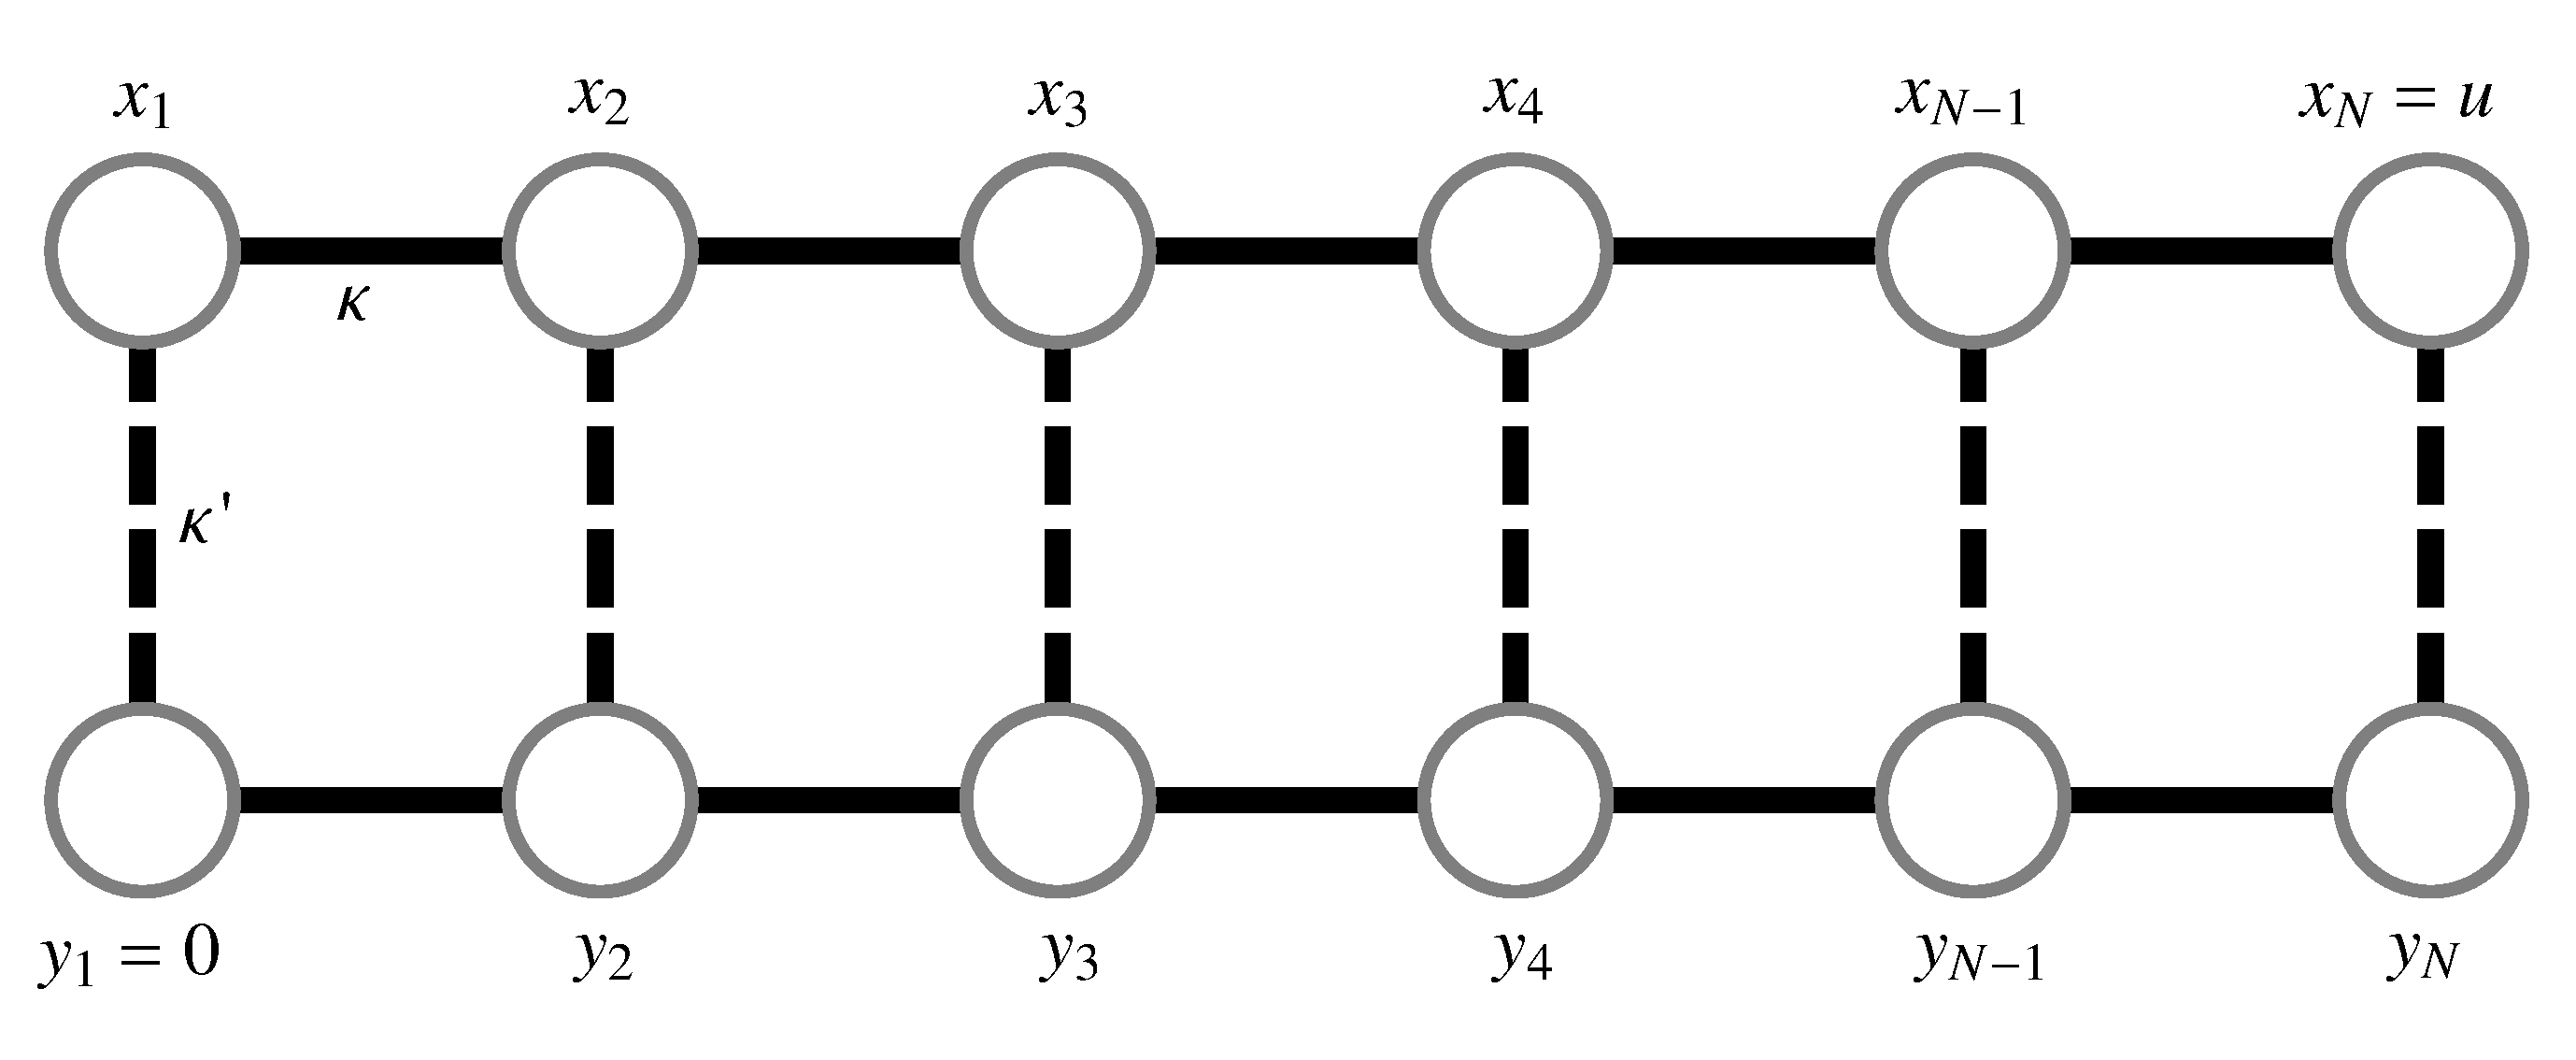
\includegraphics[scale=0.3]{Graphics/DNA_Model/dna_model_ladder.pdf}
\caption{Schematic diagram of the two dimensional ladder model for DNA.}
\label{fig:dna_model_ladder}
\end{figure}

Each particle in the ladder structure represents a nucleotide. Each stick connecting the base pairs represents the 2-3 hydrogen bonds, and each stick along the backbone represents a peptide bond connecting the nucleotides. The axial displacements of particles in each backbone are labelled $x_i$ and $y_i$, and the partners forming the $i^{th}$ base pair interact through a potential $V_{i}$ which is dependent on the axial pair separation $(x_{i}-y_{i})$. For a model that has $N$ base pairs we can write the Hamiltonian as
%
\begin{equation}
\label{dna_hamiltonian}
H = H_{x} + H_{y} + H_{bp}
\end{equation}
%
where
%
\begin{align}
\label{dna_hamiltonian_x}
H_{x} &= \sum_{i=1}^{N-1} \frac{1}{2} \kappa \left(x_{i+1}-x_{i} \right)^2 \\
\label{dna_hamiltonian_y}
H_{y} &= \sum_{i=1}^{N-1} \frac{1}{2} \kappa \left(y_{i+1}-y_{i} \right)^2 \\
\label{dna_hamiltonian_bp}
H_{bp} &= \sum_{i=1}^{N}V_{i}\left(x_{i}-y_{i}\right)
\end{align}
%
To eliminate the cross terms in the Hamiltonian we change the co-ordinate system of variables $x_{i}$ and $y_{i}$ to convert the Hamiltonian to a solvable linear system. The following substitutions transform the system to a new co-ordinate system in $\xi$ and $\eta$,
%
\begin{align}
\label{dna_transform_xi}
\xi_{i}=x_{i}+y_{i}\\
\label{dna_transform_eta}
\eta_{i}=x_{i}-y_{i}
\end{align}
%
The new Hamiltonian is now a function of $\xi$ and $\eta$
%
\begin{equation}
\label{dna_hamiltonian_xi_eta}
H\left(\xi,\eta\right) = H_{\xi} + H_{\eta} 
\end{equation}
%
where
%
\begin{align}
\label{dna_hamiltonian_xi}
H_{\xi} &= \sum_{i=1}^{N-1} \frac{\kappa}{4} \left(\xi_{i+1}-\xi_{i} \right)^2 \\
\label{dna_hamiltonian_eta}
H_{\eta} &= \sum_{i=1}^{N-1} \frac{\kappa}{4} \left(\eta_{i+1}-\eta_{i} \right)^2 + \sum_{i=1}^{N} V\left(\eta_{i}\right)
\end{align}
%
The base pairs will experience a restoring force brought about by the extension $u$ but when the bond separation goes beyond $\eta_{B}$ the force is set to zero, to begin with, signifying broken bonds as illustrated in \figref{dna_bp_pe}. 
%
\begin{align}\label{dna_pair_potential}
V_{i}\left(\eta_{i}\right)&=\frac{1}{2}\kappa'\eta_{i}^{2} \text{\hspace{5 mm}when\hspace{5 mm}}\eta_{i} \leq \eta_{B} \\
&=\frac{1}{2}\kappa'\eta_{B}^{2} \text{\hspace{5 mm}when\hspace{5 mm}}\eta_{i} > \eta_{B}\nonumber
\end{align}
%
Variations on \eqref{dna_pair_potential} can  have the base pairs experiencing either a stronger or weaker restoring force after a certain separation $\eta_{B}$, for a given extension.
%
\begin{figure}[H]
\centering
\begin{tabular}{cc}
\subfloat[]{\label{fig:dna_model_3dladder}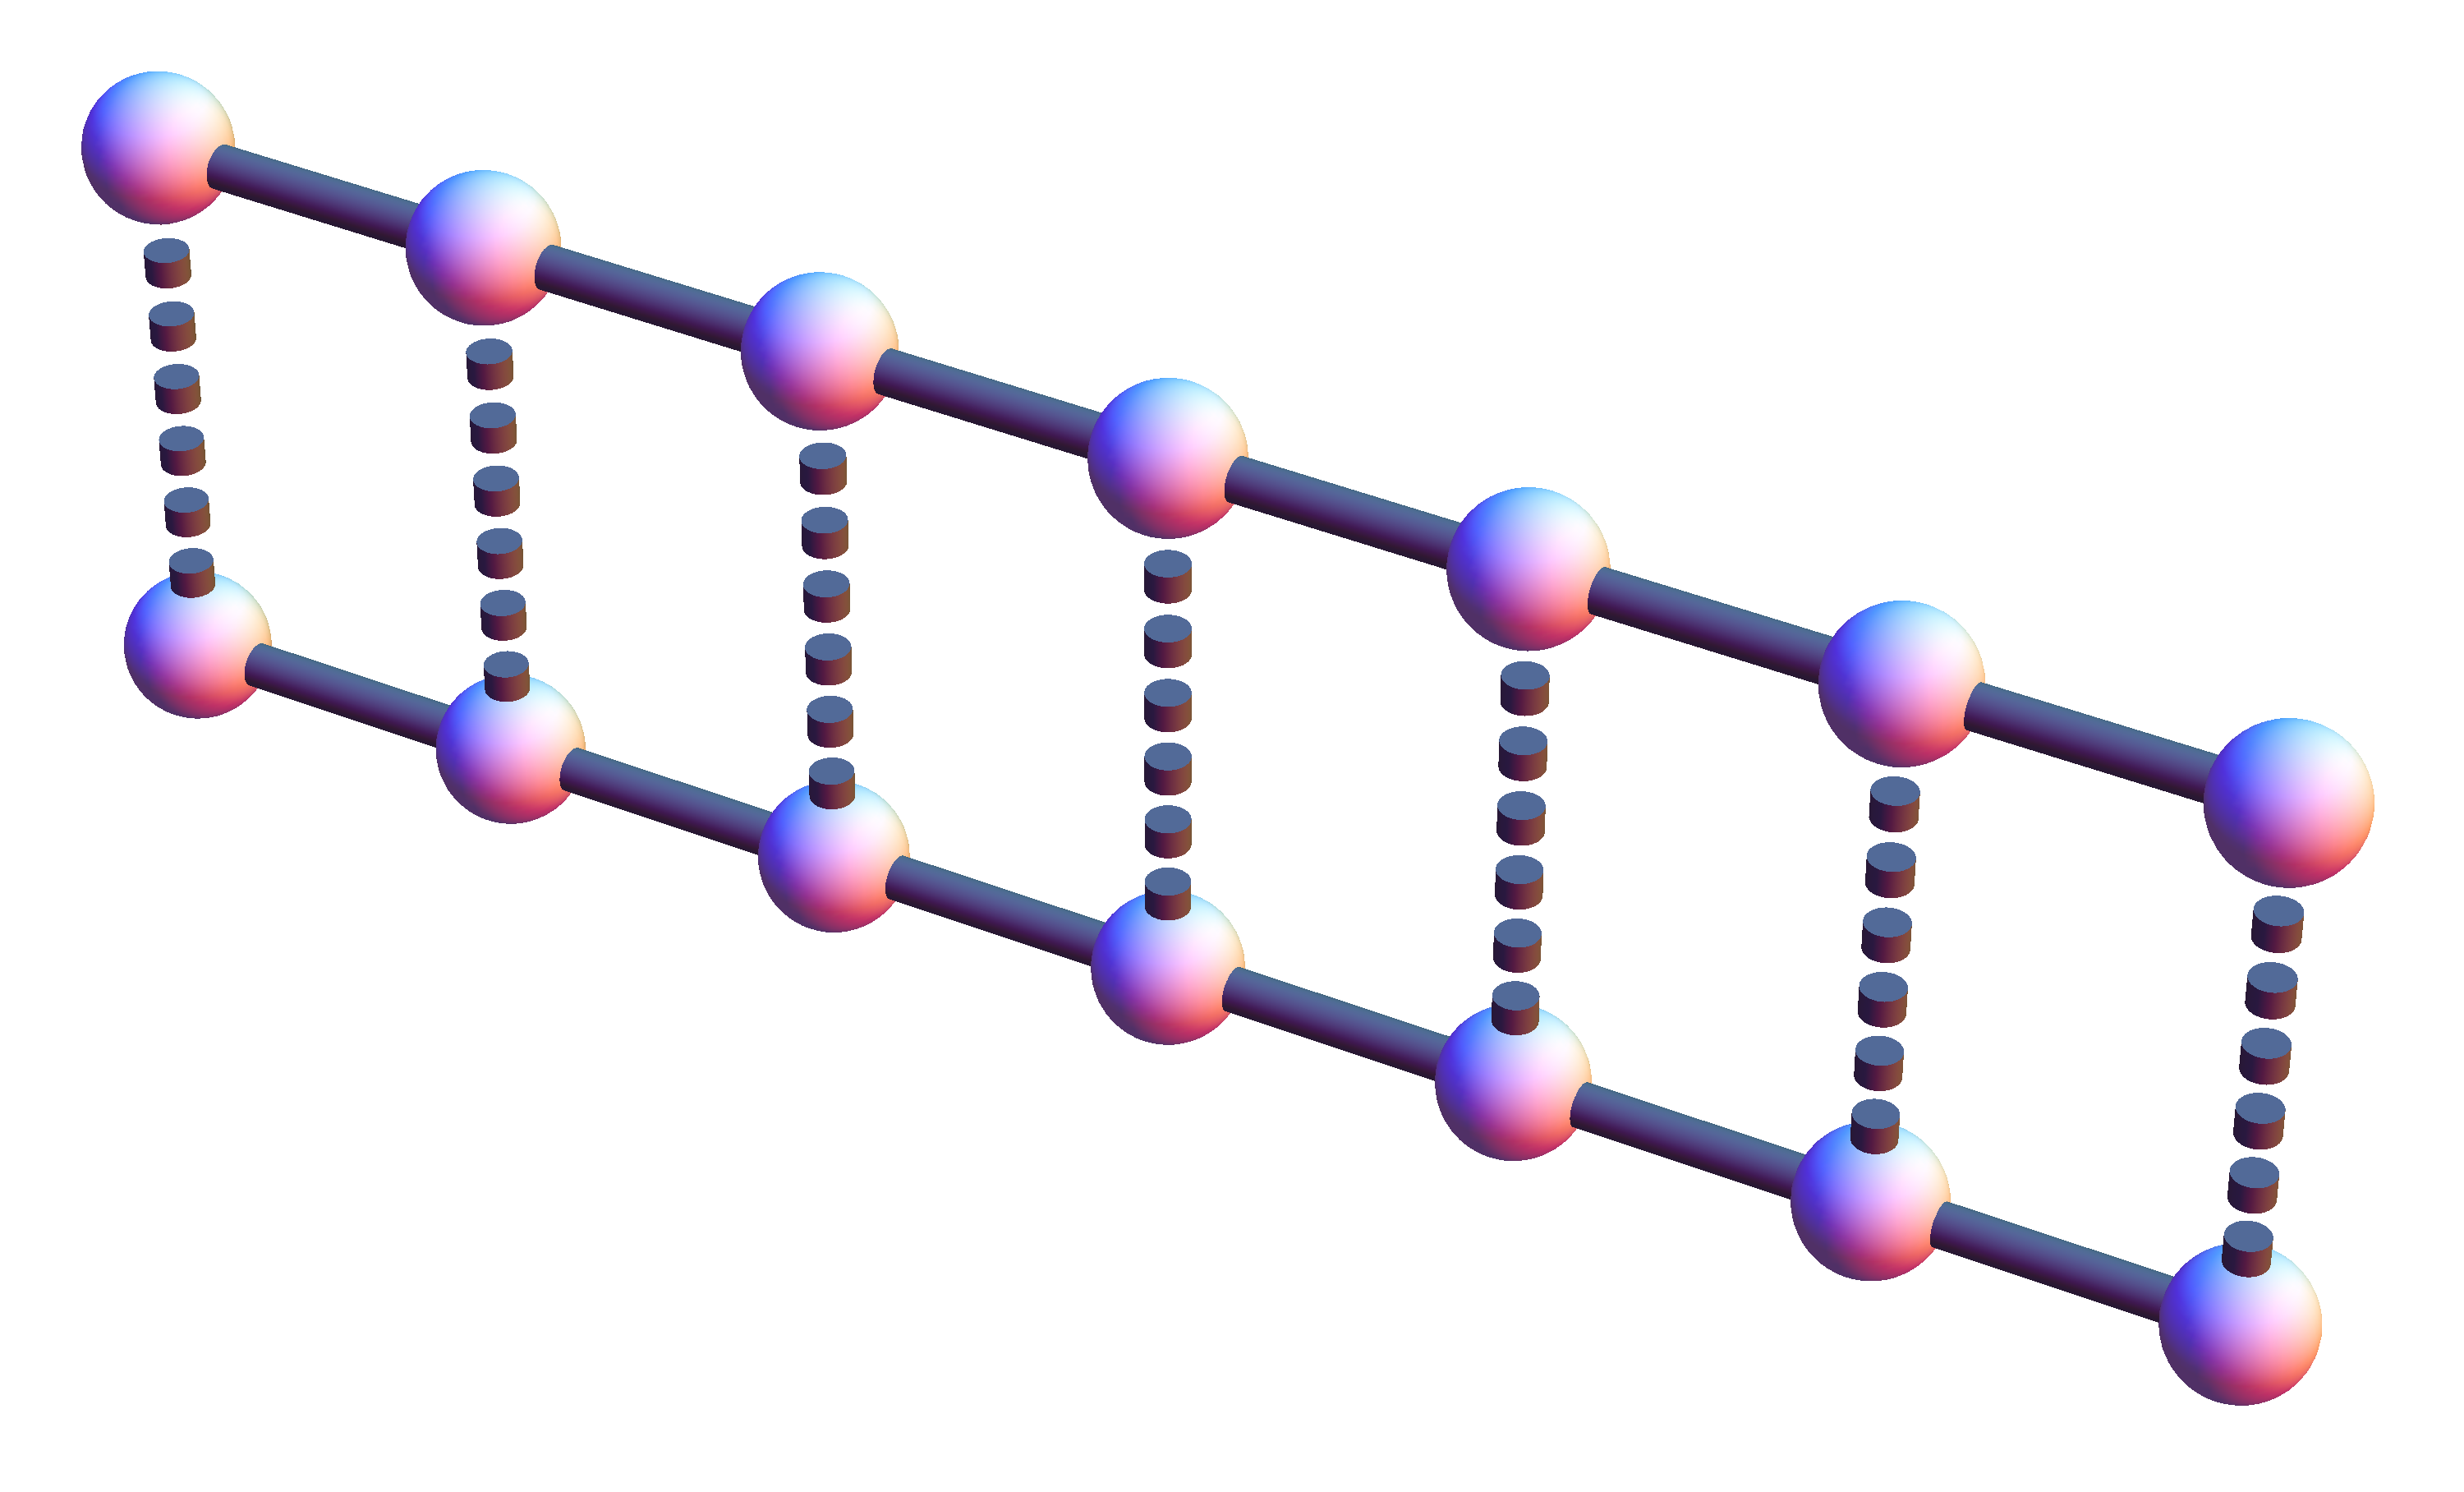
\includegraphics[scale=0.11]{Graphics/DNA_Model/dna_model_3d_ladder.pdf}} &
\subfloat[]{\label{fig:dna_model_3dladder_pulled}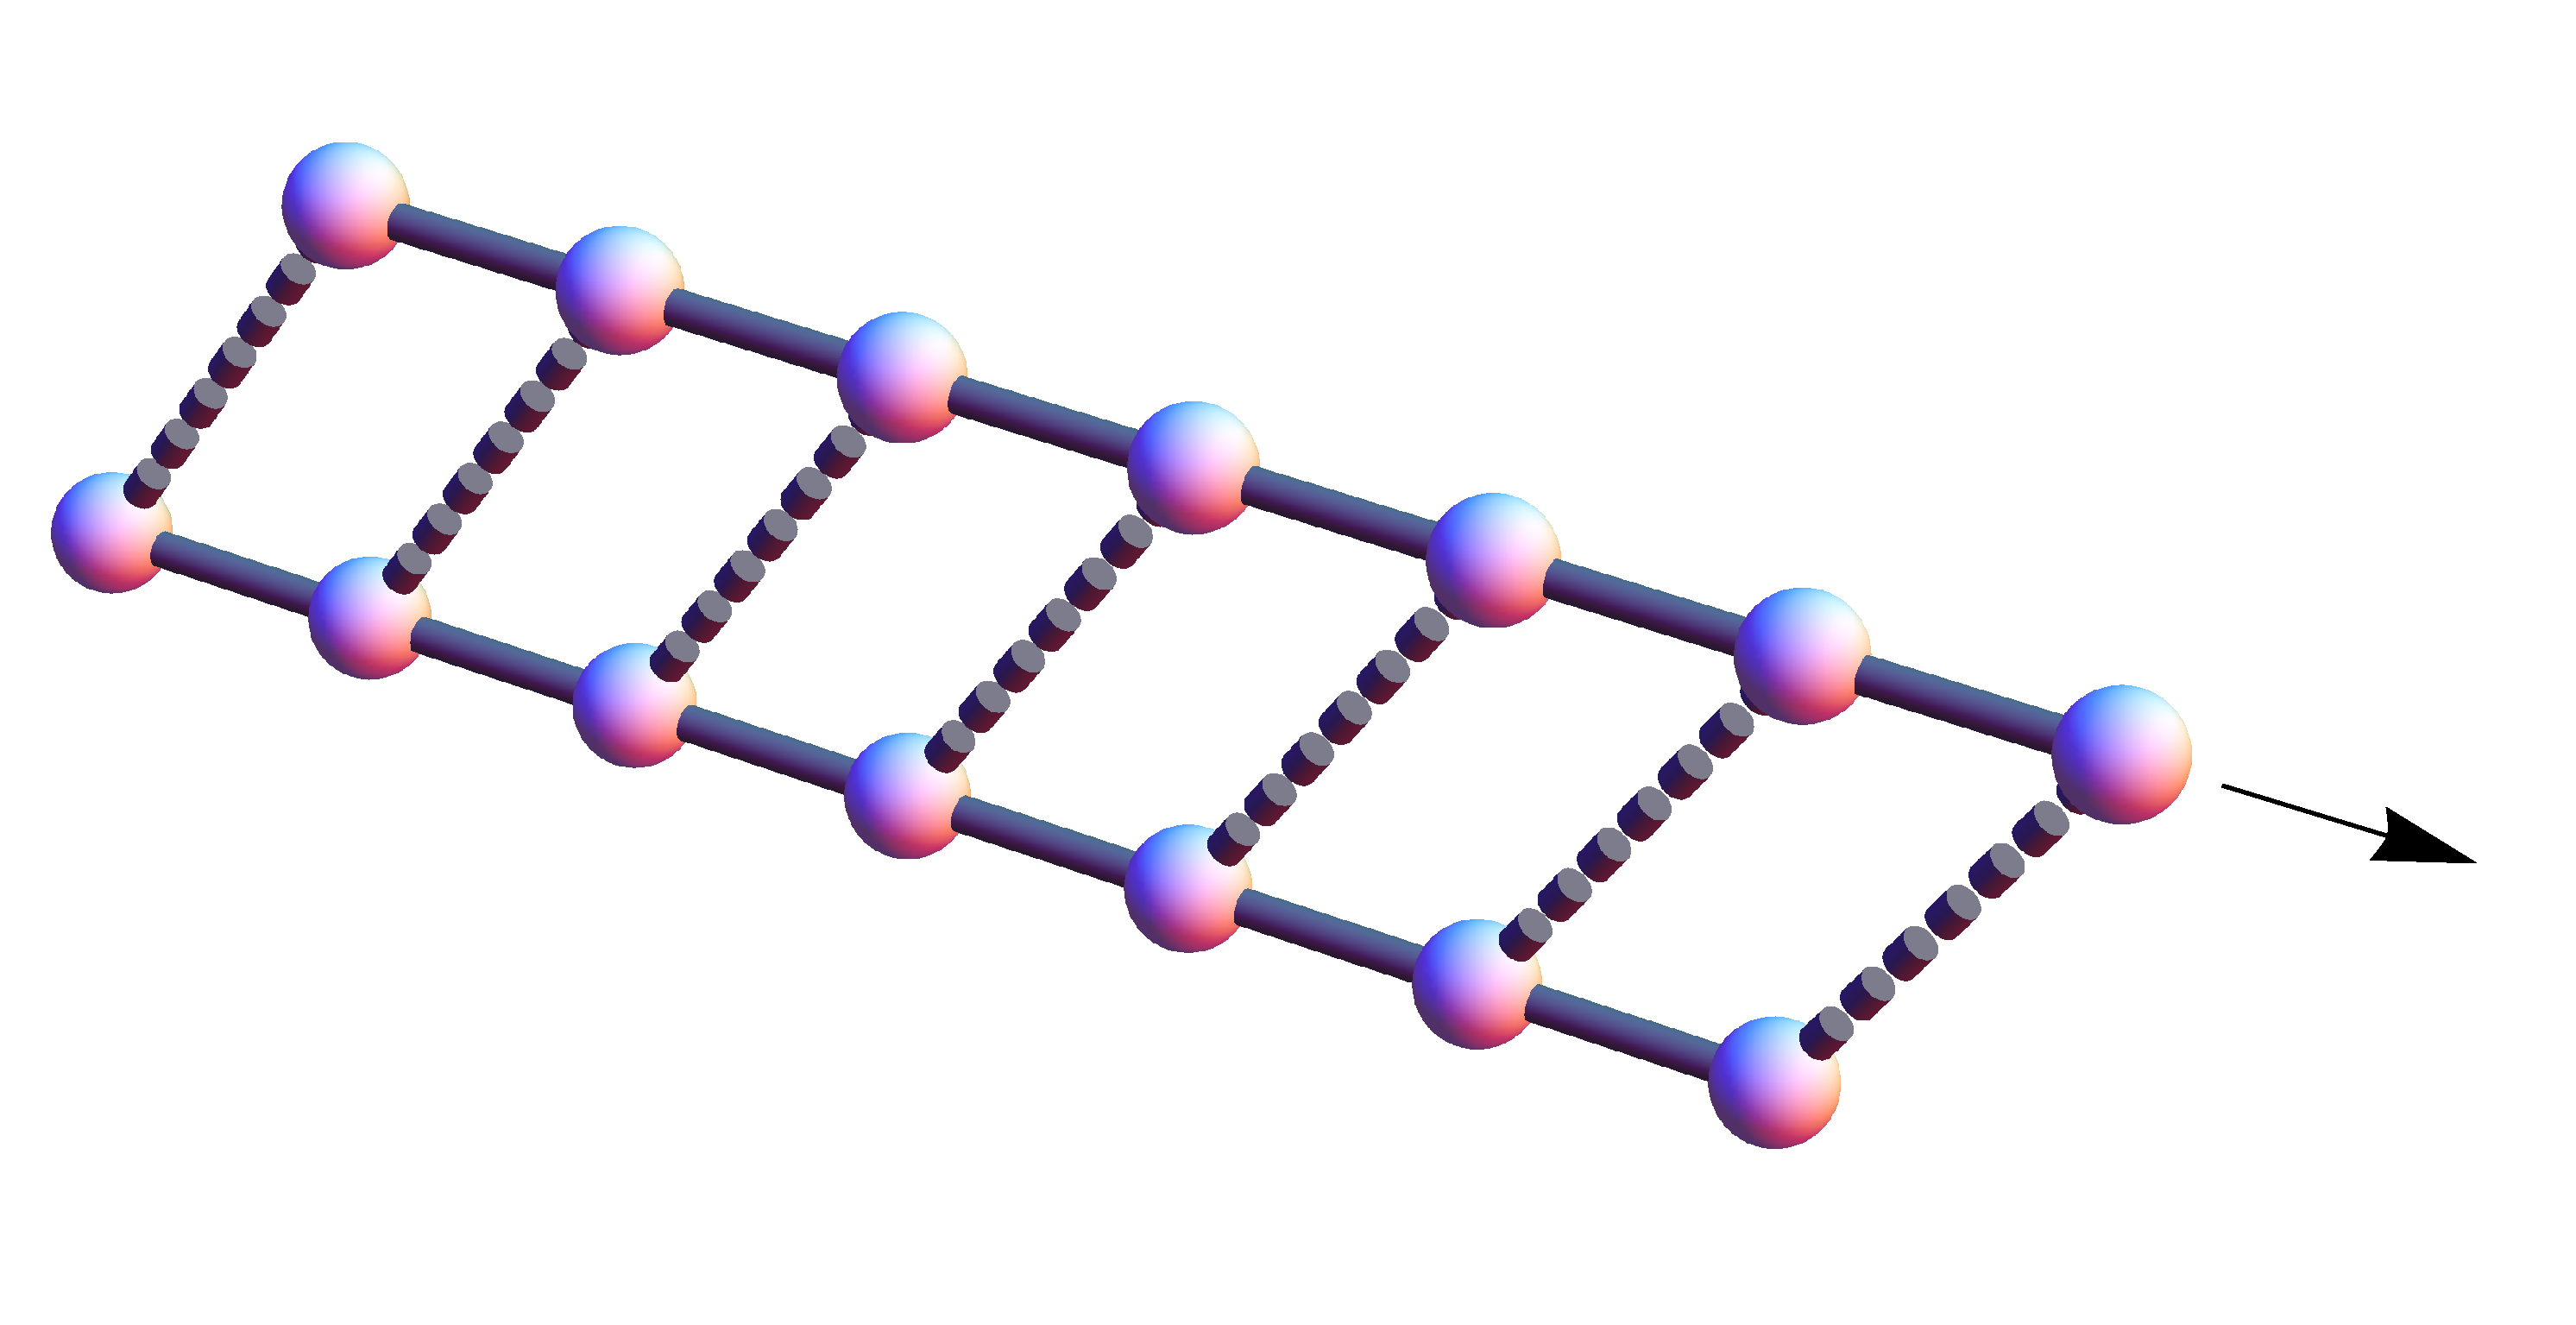
\includegraphics[scale=0.15]{Graphics/DNA_Model/dna_model_3d_ladder_pulled.pdf}} 
\end{tabular} 
\caption{A three-dimensional illustration of the DNA ladder model. In \figref{dna_model_3dladder} we have an intact ladder structure that hasn't been influenced by axial extension. When an extension is applied to the ladder structure from one end as illustrated in \figref{dna_model_3dladder_pulled} the base pairs tilt towards the displacement end, experiencing a restoring force defined by the base pair potential.}
\label{fig:dna_3d}
\end{figure}
%
\begin{figure}[H]
\centering
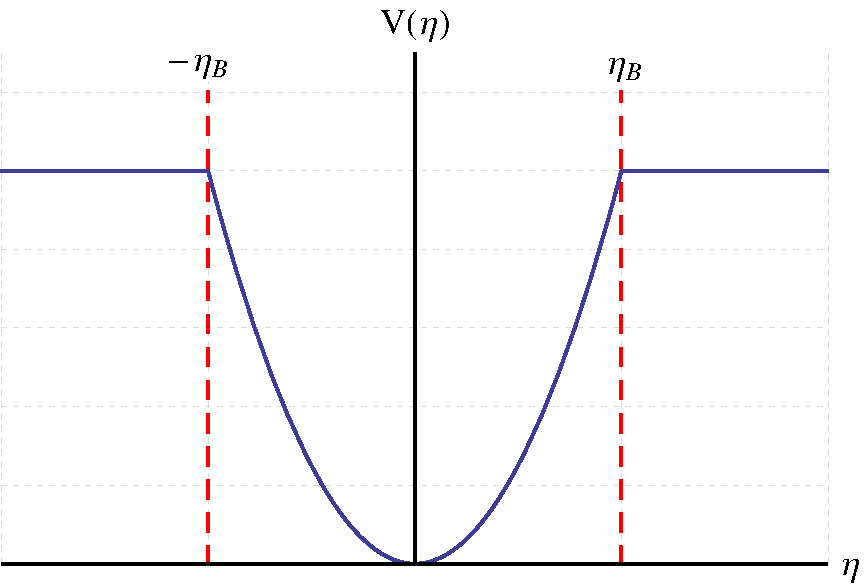
\includegraphics[scale=0.6]{Graphics/DNA_Model/basepair_potential.pdf}
\caption{A plot of the base pair potential as described by \eqref{dna_pair_potential}.} 
\label{fig:dna_bp_pe}
\end{figure}
%


\section{Partition Function Integral}

The separation of variables in the Hamiltonian allows us to evaluate the partition function for various breakage patterns. We can neglect the momentum part of the Hamiltonian as we already shown in the EFJC that this only contributes a constant factor. The partition function integral is evaluated over phase-space $d\tau=d\xi\,d\eta$ per base pair. For a $N$ base pair system we have a multi-dimensional partition function integral
%
\begin{equation}
\label{dna_partition_function}
Z=\int \prod^{N}_{i=1}d\xi_{i}\,d\eta_{i}\exp\left(-\beta H\left(\xi_{i},\eta_{i}\right)\right)
\end{equation}
%
Where $\beta=\frac{1}{k_{B}T}$. We simplify the Hamiltonian \eqref{dna_hamiltonian_xi_eta} further by converting $\xi$ and $\eta$ into dimensionless quantities such that $\xi \to \xi\left(\frac{\kappa\beta}{4}\right)^{-\frac{1}{2}}$, and $\eta \to \eta\left(\frac{\kappa\beta}{4}\right)^{-\frac{1}{2}}$.  The Hamiltonian becomes
%
\begin{equation}
\label{dna_betaH}
\beta H = \sum_{i=1}^{N-1} \left(\xi_{i+1}-\xi_{i} \right)^2 + \sum_{i=1}^{N-1} \left(\eta_{i+1}-\eta_{i} \right)^2 + \sum_{i=1}^{N} V\left(\eta_{i}\right)
\end{equation}
%
and the base pair potential \eqref{dna_pair_potential} becomes a function of dimensionless $\eta$
%
\begin{align}
\label{dimensionless_dna_pair_potential}
V\left(\eta\right)&=\frac{2 \kappa'}{\kappa}\eta^{2} \text{\hspace{5 mm}when\hspace{5 mm}}\eta \leq \eta_{B} \\
&=\frac{2 \kappa'}{\kappa}\eta_{B}^{2} \text{\hspace{5 mm}when\hspace{5 mm}}\eta > \eta_{B}\nonumber
\end{align}
%
Applying the transformation to the partition function \eqref{dna_partition_function} creates a constant $\left(\frac{\kappa\beta}{4}\right)^{N}$ in front of the integral which is ignored from the calculation. Like the momentum part of the partition function integral it doesn't affect the behaviour of the free energy curves, and therefore has no impact on the force-extension calculations. 

\section{Transfer Matrices}

To express $Z$ in terms of transfer matrices we focus our attention on the exponential term in the partition function.  We insert \eqref{dna_betaH} into \eqref{dna_partition_function} and make an expansion of the $\exp\left(-\beta H\right)$ term.  We are then able to group like terms together and adjust the exponentials such that they are symmetric in both $\xi$ and $\eta$:
%
\begin{align}
\label{dna_rearranged_expo}
\exp\left(-\beta H\right)&=\prod_{i=1}^{N-1}\exp\left(-\left(\xi_{i+1}-\xi_{i}\right)^{2}\right)\nonumber\\
&\times\prod_{j=1}^{N-1}\exp\left(-\left(\eta_{j+1}-\eta_{j}\right)^2 + \left(\frac{V\left(\eta_{i+1}\right)+V\left(\eta_{i}\right)}{2}\right)\right)\nonumber\\
&\times\exp\left(-\frac{V\left(\eta_{1}\right)+V\left(\eta_{N}\right)}{2}\right)
\end{align}
%
We can now introduce a set of transfer matrices for both $\xi$ and $\eta$
%
\begin{align}
\label{dna_tm_xi}
T\left(\xi_{i+1},\xi_{i}\right) &= \exp\left(-\left(\xi_{i+1}-\xi_{i}\right)^{2}\right)\\
\label{dna_tm_eta}
\hat{T}\left(\eta_{i+1},\eta_{i}\right) &= \exp\left(-\left(\eta_{j+1}-\eta_{j}\right)^2 - \left(\frac{V\left(\eta_{i+1}\right)+V\left(\eta_{i}\right)}{2}\right)\right)
\end{align}
%
When we talk about the breakage patterns in DNA we are actually referring to patterns of broken base pairs. Two types of breakage patterns occur in DNA, fraying and bubbling.  Fraying occurs when the base pairs break from the ends of the DNA molecule \figref{dna_frayed}, and bubbling occurs when base pairs break from within the DNA molecule \figref{dna_bubble}. 
%
\begin{figure}[htp]
\centering
\begin{tabular}{cc}
\subfloat[$\{\mu\}=\{0,0,0,0,0,1\}$]{\label{fig:dna_frayed_1}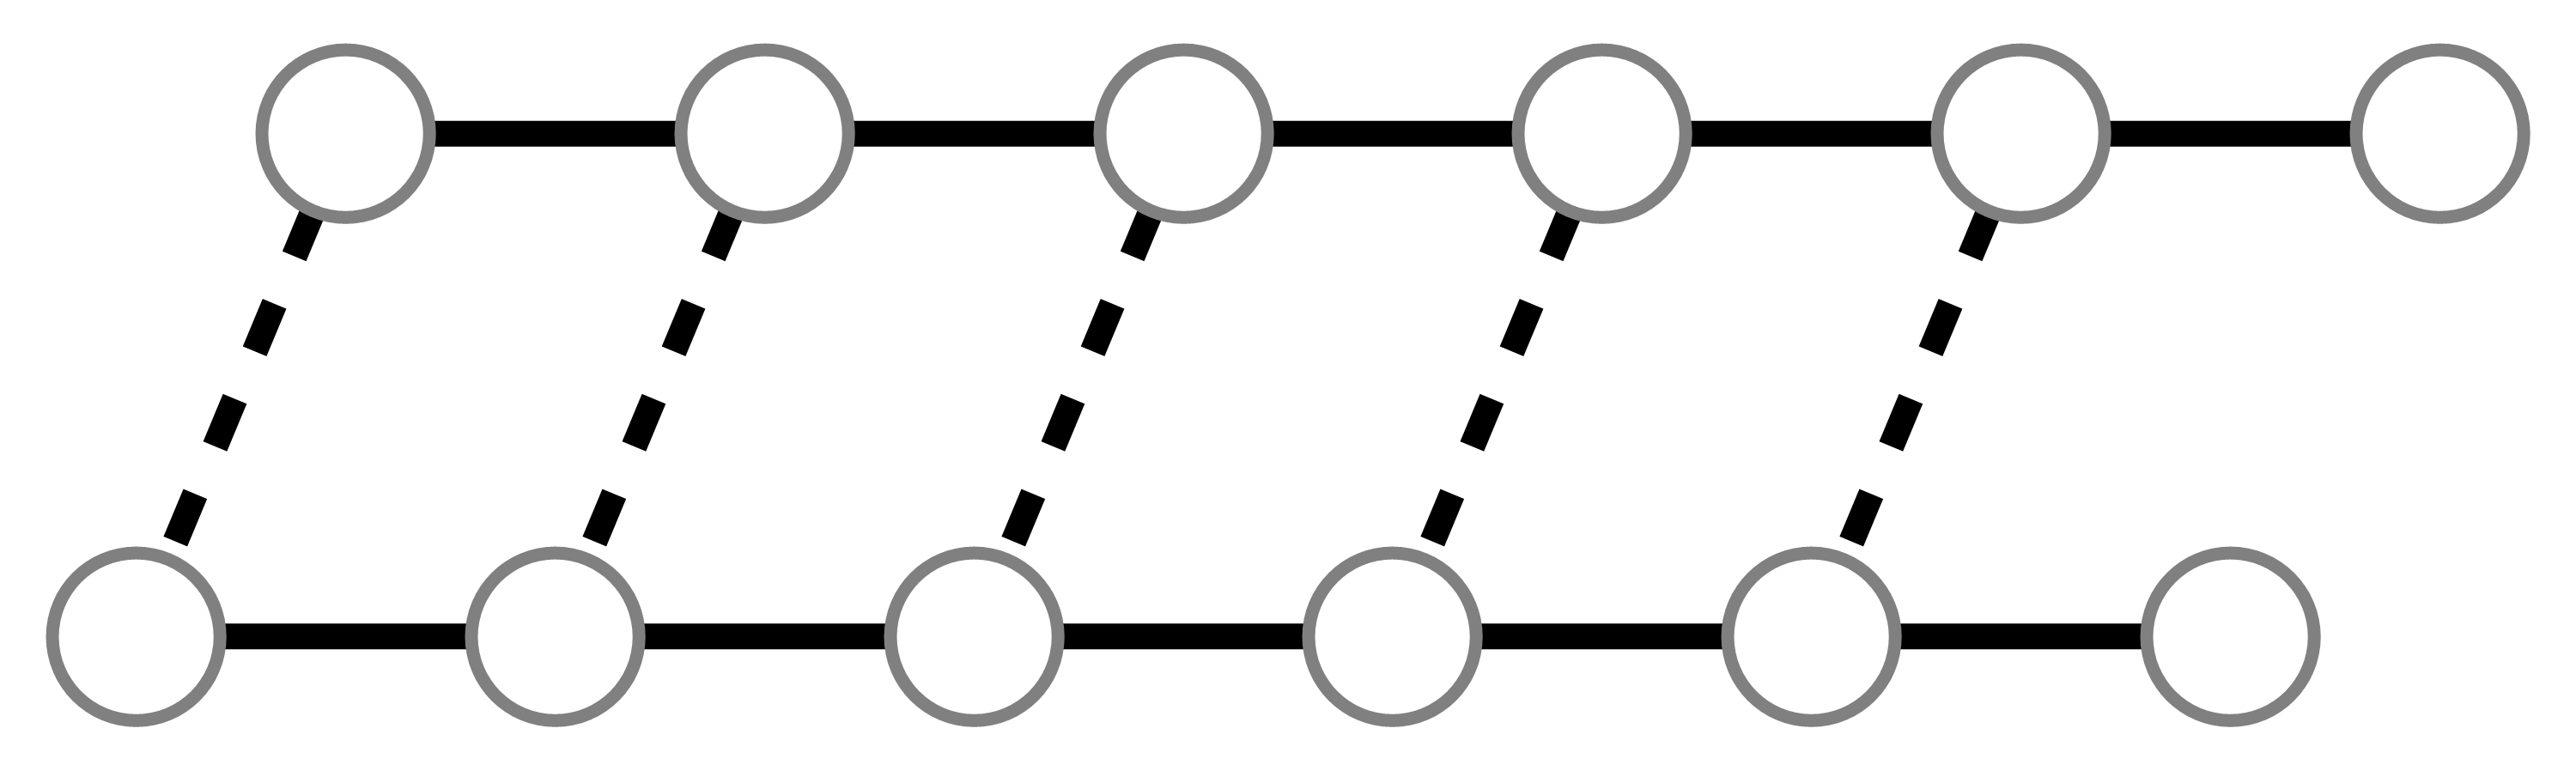
\includegraphics[scale=0.275]{Graphics/DNA_Model/dna_frayed_1.pdf}} \\
\subfloat[$\{\mu\}=\{0,0,0,0,1,1\}$]{\label{fig:dna_frayed_2}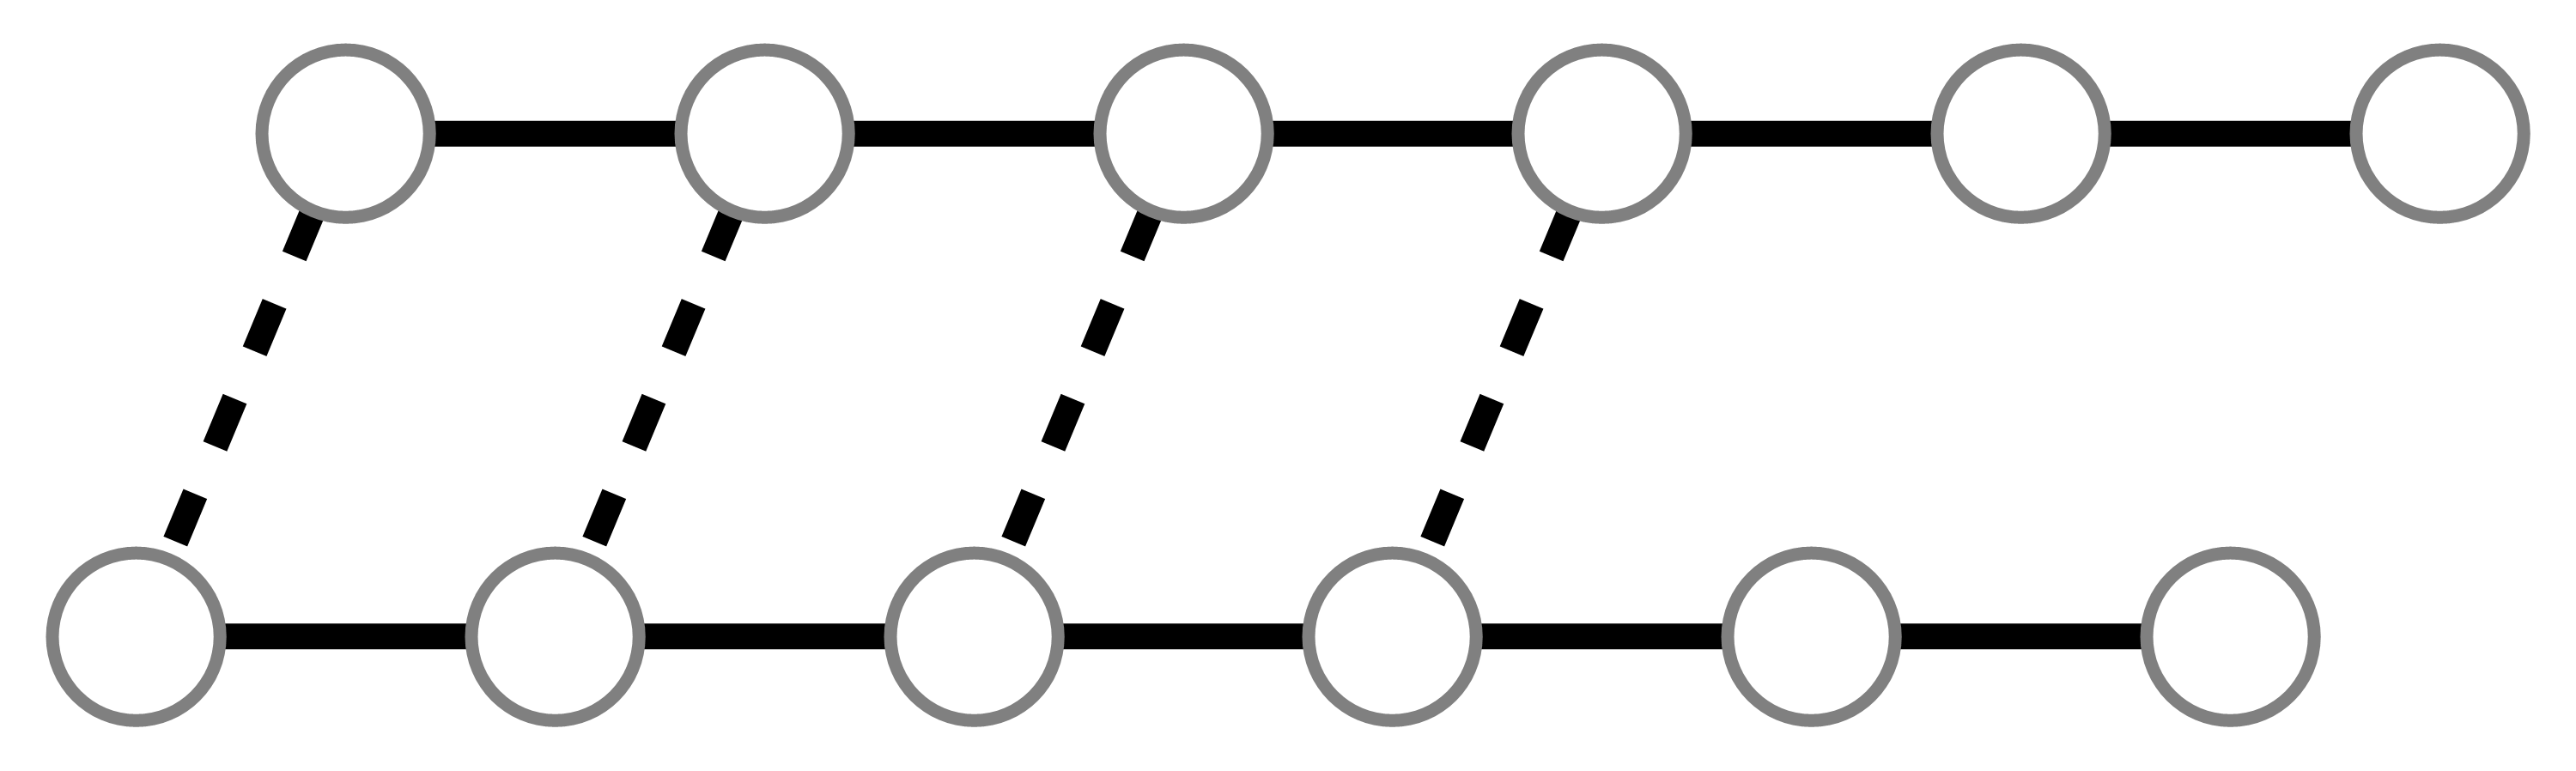
\includegraphics[scale=0.275]{Graphics/DNA_Model/dna_frayed_2.pdf}} 
\end{tabular} 
\caption{Different frayed states in DNA for $N=6$.}
\label{fig:dna_frayed}
\end{figure}
%
\begin{figure}[htp]
\centering
\begin{tabular}{cc}
\subfloat[$\{\mu\}=\{0,0,1,0,0,0\}$]{\label{fig:dna_bubble_1}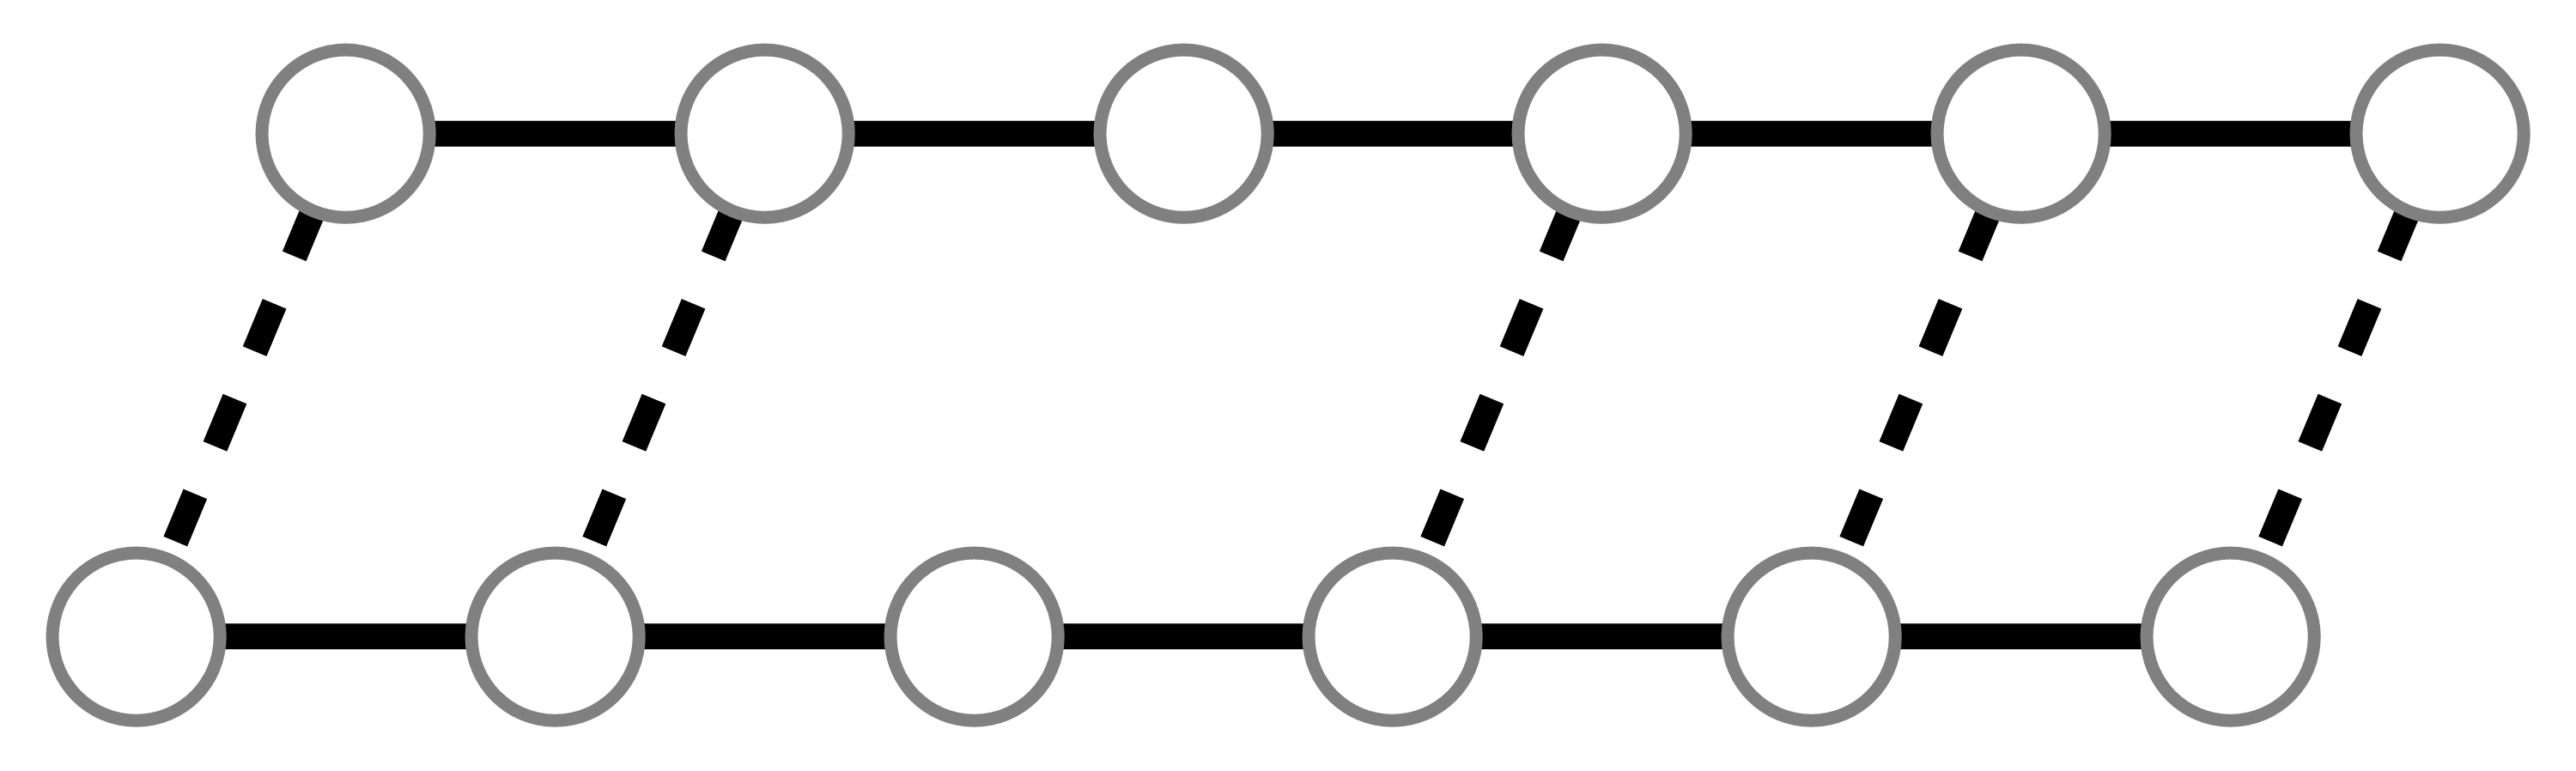
\includegraphics[scale=0.275]{Graphics/DNA_Model/dna_bubble_1.pdf}}\\
\subfloat[$\{\mu\}=\{0,0,1,1,0,0\}$]{\label{fig:dna_bubble_2}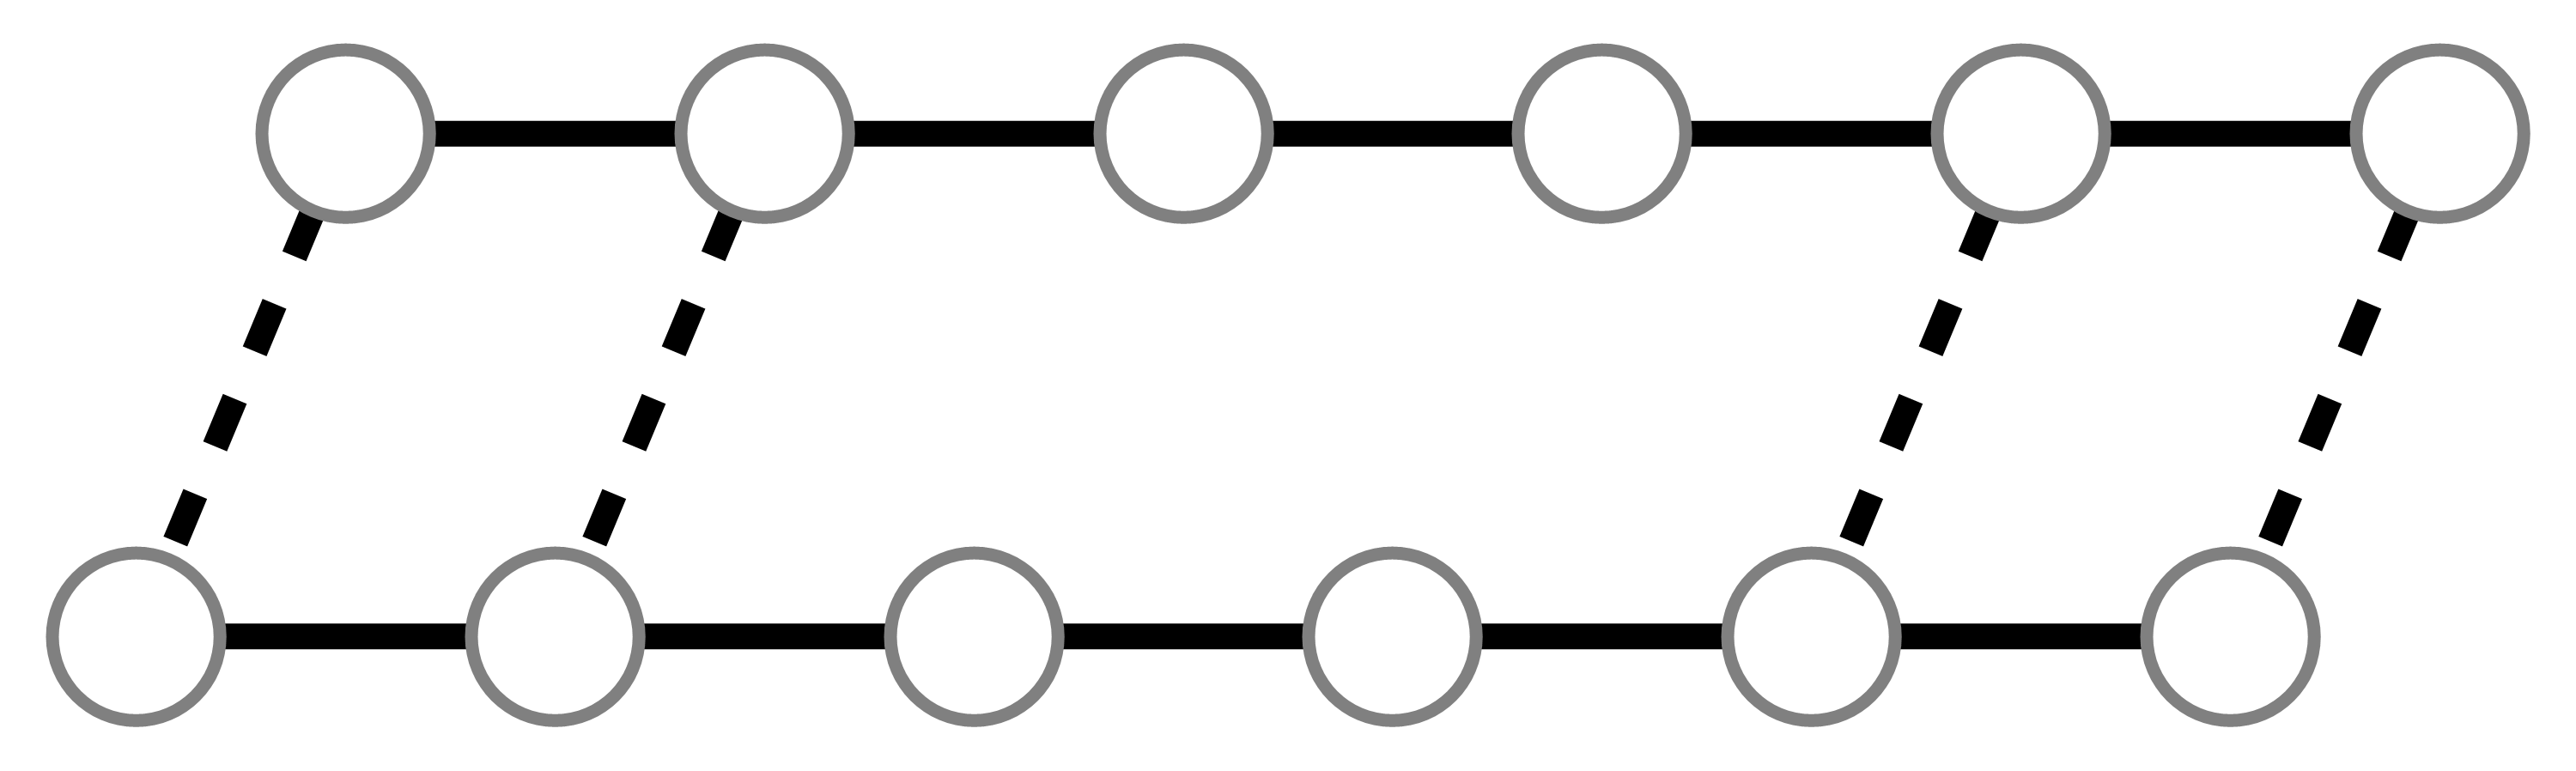
\includegraphics[scale=0.275]{Graphics/DNA_Model/dna_bubble_2.pdf}}
\end{tabular} 
\caption{Different bubbled states in DNA for $N=6$.}
\label{fig:dna_bubble}
\end{figure}
%
To calculate the free energies of various breakage patterns we need to incorporate these breakage patterns into the DNA ladder model by a modification of the transfer matrices. We can do this by introducing a bond breakage criterion embodied in a $g$ factor, $g_{\mu}$. Here the label $\mu$ indicates whether a base pair is either intact ($\mu=0$), or  broken ($\mu=1$). Since these breakage patterns only apply to the base pairs we can insert the following factors as a function of $\eta$ into the transfer matrices, $\hat{T}$. For an intact base pair 
%
\begin{align}
\label{dna_g0}
g_{0}\left(\eta\right)&=1 \hspace{5mm} \text{if} \hspace{5mm} |\eta | \leq \eta_{B}\\
&=0 \hspace{5mm} \text{Otherwise}\nonumber
\end{align}
%
For a broken base pair the $g$ factor becomes,
%
\begin{align}
\label{dna_g1}
g_{1}\left(\eta\right)&=1 \hspace{5mm} \text{if} \hspace{5mm} |\eta | > \eta_{B}\\
&=0 \hspace{5mm} \text{Otherwise}\nonumber
\end{align}
%
Inserting these factors makes the following transformation of the transfer matrix, $\hat{T} \to \hat{T}_{\mu_{i},\mu_{i+1}}$, such that
%
\begin{equation}
\label{dna_t_hat_matrix}
\hat{T}_{\mu_{i},\mu_{i+1}}\left(\eta_{i},\eta_{i+1}\right) = g_{\mu_{i}}\left(\eta_{i}\right)g_{\mu_{i+1}}\left(\eta_{i+1}\right) \exp\left(-\left(\eta_{i+1}-\eta_{i}\right)^2 - \left(\frac{V\left(\eta_{i+1}\right)+V\left(\eta_{i}\right)}{2}\right)\right)
\end{equation}
%
The partition function integral can now be expressed as a product of transfer matrices
%
\begin{align}
Z&=\int \prod_{i=1}^{N}d\xi_{i}\,\left(\prod_{i'=1}^{N-1}T\left(\xi_{i'+1},\xi_{i'}\right)\right)\nonumber\\
&\times\int \prod_{j=1}^{N}d\eta_{j}\,\left(\prod_{j'=1}^{N-1}\hat{T}_{\mu_{j'},\mu'_{j'+1}}\left(\eta_{j'},\eta_{j'+1}\right)\right)\exp\left(-\frac{V\left(\eta_{1}\right)+V\left(\eta_{N}\right)}{2}\right)
\end{align}
%
This partition function constructed out of transfer matrices can be simplified if we somehow provide eigenfunctions that allow the expression to be contracted. We next look at how these eigenfunctions arise from the boundary conditions of the system.
%
\section{Boundary Conditions}
%
The boundary conditions in the ladder structure are applied to the partition function through a set of delta functions: the particle at the position $y_{1}$ is fixed by the insertion of $\delta\left(y_{1}\right)$ such that it remains in equilibrium, and the particle at the pulled end is constrained to take the extension $u$ from its original position $\delta\left(x_{N}-u\right)$. In the new co-ordinate system the boundary conditions are transformed by \eqref{dna_hamiltonian_xi} and \eqref{dna_hamiltonian_eta} to
%
\begin{equation}
\delta\left(y_{1}\right)\delta\left(x_{N}-u\right) = \delta\left(\xi_{1}-\eta_{1}\right)\delta\left(\xi_{N}+\eta_{N}-2u\right)
\end{equation}
%
\section{Eigenvalue Equations}
%
The transfer integral method simplifies the partition function calculation of the DNA model to the solutions of a set of eigenvalue equations. We saw in the Ising model in chapter 3 that the transfer operators contain all the information needed to describe how the spins were distributed and correlated with their neighbours. In the DNA model the transfer operators provides information on whether a base pair is broken or intact, and the effects of the potential at a given extension. The eigenfunctions needed to contract the transfer matrices come from the expansion of the delta functions that impose the boundary conditions. 
%
\begin{align}
\label{dna_delta_1}\delta\left(\xi_{1}-\eta_{1}\right)&=\sum_{t}\hat{\psi}^{*}_{t}\left(\xi_{1}\right)\hat{\psi}_{t}\left(\eta_{1}\right)\\
\label{dna_delta_2}\delta\left(\xi_{N}+\eta_{N}-2u\right)&=\sum_{s}\psi^{*}_{s}\left(2u-\xi_{N}\right)\psi_{s}\left(\eta_{N}\right)
\end{align}
%
We introduce $\psi_{s}$, eigenfunctions of the transfer matrix \eqref{dna_tm_xi}, and $\hat{\psi}_{t}$, the eigenfunctions of the transfer matrix \eqref{dna_tm_eta}. The eigenfunctions satisfy the eigenvalue equations for the backbone $T$, intact base pair $\hat{T}_{00}$, and a broken base pair $\hat{T}_{11}$ transfer matrices by
%
\begin{align}
\label{dna_eign_t}
\int \,d\xi'T\left(\xi,\xi'\right)\psi_{s}\left(\xi'\right) &= \lambda_{s}\psi_{s}\left(\xi\right) \\
\label{dna_eign_hat}
\int \,d\eta'\hat{T}_{00}\left(\eta,\eta'\right)\hat{\psi}_{t}\left(\eta'\right) &= \hat{\lambda}_{t}\hat{\psi}_{t}\left(\eta\right) \\
\label{dna_eign_twidle}
\int \,d\eta'\hat{T}_{11}\left(\eta,\eta'\right)\tilde{\psi}_{v}\left(\eta'\right) &=\tilde{ \lambda}_{v}\tilde{\psi}_{v}\left(\eta\right)
\end{align}
%
respectively. Using these eigenvalue equations we are able to contract the expression for $Z$ transfer matrices leaving a sum involving eigenvalues and eigenvectors. Numerically the eigenfunctions can be calculated if we discretise the transfer matrix; however, in certain cases analytical solutions can be found. 
%
\subsection{Analytical solutions for eigenvectors and eigenvalues of $T$}

If we take a closer look at \eqref{dna_tm_xi} we find that $T$ is just a Gaussian function, and thus \eqref{dna_eign_t} can be solved analytically to give solutions for $\psi_{s}$ and $\lambda_{s}$. The integral equation becomes
%
\begin{equation}
\label{ana_s_sol1}
\int \,d\xi'\exp\left(-\left(\xi'-\xi\right)^{2}\right)\psi_{s}\left(\xi'\right) = \lambda_{s}\psi_{s}\left(\xi\right)
\end{equation}
%
By assuming the eigenfunction is of the form $\psi_{s}\left(\xi\right)=A\exp\left(is \xi B\right)$ where $A$ and $B$ are constants the integral equation becomes
%
\begin{equation}
\label{ana_s_sol2}
\int \,d\xi'\exp\left(-\left(\xi-\xi'\right)^{2}\right)A\exp\left(is \xi' B\right) = \lambda_{s}\psi_{s}\left(\xi\right)
\end{equation}
%
Then making a substitution $\gamma=\xi-\xi'$ we get
%
\begin{equation}
\label{ana_s_sol3}
-A\exp\left(is \xi B\right)\int \,d\gamma\exp\left(-\gamma^{2}\right)\exp\left(-is \gamma B\right) = \lambda_{s}\psi_{s}\left(\xi\right)
\end{equation}
%
and we find that the integral is simply a Fourier transform of the Gaussian function
%
\begin{equation}
\label{ana_s_sol4}
\int_{-\infty}^{\infty}\exp\left(-\alpha x^2\right)\exp\left(-ivx\right)dx=\sqrt{\frac{\pi}{\alpha}}\exp\left(-\frac{v^{2}}{4\alpha}\right)
\end{equation}
%
Using this transformation we get
%
\begin{equation}
\label{ana_s_sol5}
-A\exp\left(is \xi B\right)\left(\sqrt{\pi}\exp\left(-\frac{B^{2}s^{2}}{4}\right)\right) = \lambda_{s}\psi_{s}\left(\xi\right)
\end{equation}
%
Hence
\begin{equation}
\lambda_{s}=\sqrt{\pi}\exp\left(-\frac{B^{2}s^{2}}{4}\right)
\end{equation}
%
All that remains is to find the constant $B$.  Here we impose periodicity such that we can represent the $\psi_{s}$ eigenfunction on a finite spatial range $L$. At this point we also take $s$ to be an integer label. We impose
%
\begin{equation}
\psi_{s}\left(\alpha +L\right)=\psi_{s}\left(\alpha\right)
\end{equation}
%
such that
%
\begin{equation}
\exp\left(isB\left(\alpha+L\right)\right)=\exp\left(isB\alpha\right)
\end{equation}
%
or
%
\begin{equation}
\exp\left(isBL\right)=1
\end{equation}
%
Since $\exp\left(is2\pi\right)=1$, we can substitute that on the RHS, and take the logarithmic of both sides. This result gives
%
\begin{equation}
\label{ana_s_sol_const_B}
B=\frac{2\pi}{L}
\end{equation}
%
To find the constant $A$ we simply use the normalisation condition. Integrating over finite range from $-\frac{L}{2}$ to $\frac{L}{2}$, we get
%
\begin{align}
\label{ana_s_sol_norm}
\int_{-\frac{L}{2}}^{\frac{L}{2}}|\psi_{s}\left(\xi\right)|^{2}\,d\xi&=1\\
|A|^{2}L&=1
\end{align}
%
Hence
\begin{equation}
\label{ana_s_sol_const_A}
A=L^{-\frac{1}{2}}
\end{equation}
%
Thus the $T$ transfer matrix has eigenfunctions that are expressed as
%
\begin{equation}
\label{dna_T_eigenfunction}
\psi_{s}\left(\xi\right)=L^{-\frac{1}{2}}\exp\left(\frac{i s 2\pi\xi}{L}\right)
\end{equation}
%
with corresponding eigenvalues
%
\begin{equation}
\label{dna_T_eigenvalue}
\lambda_{s}=\pi^{\frac{1}{2}}\exp\left(-\frac{\pi^{2} s^{2}}{L^{2}}\right)
\end{equation}
%
We are now able to make some simplifications to the delta function expansion of \eqref{dna_delta_2} where the analytical form of the eigenfunction $\psi_{s}$ allows us to take out extension parameter $u$ to become
%
\begin{equation}
\psi^{*}_{s}\left(2u-\xi_{N}\right)=\exp\left(-\frac{i4\pi s u}{L}\right)\psi_{s}\left(\xi_{N}\right)
\end{equation}
%
The delta function expansion of \eqref{dna_delta_2} can now be expressed as
%
\begin{align}
\label{dna_delta_2b}
\delta\left(\xi_{N}+\eta_{N}-2u\right)&=\sum_{s}\exp\left(-\frac{i4\pi s u}{L}\right)\psi_{s}\left(\xi_{N}\right)\psi_{s}\left(\eta_{N}\right)
\end{align}
%
\subsection{Analytical solutions for eigenvectors and eigenvalues of $\hat{T}$}

The $g$ factors in \eqref{dna_t_hat_matrix} make it inconvenient to find analytical solutions for $\hat{\psi}_{t}$ and $\hat{\lambda}_{t}$ except for a special case when $\eta_{b} \to \infty$ for intact base pairs. In this limit the $g$ factors become unity reducing the transfer matrix equation $\hat{T}_{00}$ to $\hat{T}$, as given in \eqref{dna_tm_eta}. The simplification of the transfer matrix means we are able to solve the eigenvalue equation by inserting $\hat{T}$ into \eqref{dna_eign_hat}.
%
\begin{equation}
\int \,d\eta'\exp\left(-\left(\eta-\eta'\right)^2 - \frac{\kappa'}{\kappa}\left(\eta^{2}+\eta'^{2}\right)\right)\hat{\psi}_{t}\left(\eta'\right) = \hat{\lambda}_{t}\hat{\psi}_{t}\left(\eta\right)
\end{equation}
%
This integral is very similar to a Gaussian integral which therefore indicates that $\hat{\psi}_{t}$ might must be a Gaussian in some form. We assume that
%
\begin{equation}
\label{dna_assu_med_eigen}
\hat{\psi}_{t}\left(\eta'\right)=A\exp\left(-\frac{B}{2}\eta'^{2}\right)
\end{equation}
%
where A and B are unknown constants. If we collect the like terms together our eigenvalue equation becomes
%
\begin{equation}
\label{dna_t_int}
A\int \,d\eta'\exp\left(-\eta^{2}\left(\frac{\kappa+\kappa'}{\kappa}\right)-2\eta\eta' -\eta'^{2}\left(1+\frac{2\kappa'+\kappa\left(B+2\right)}{2\kappa}+\frac{B}{2}\right)\right) = \hat{\lambda}_{t}\hat{\psi}_{t}\left(\eta\right)
\end{equation}
%
which is a Gaussian integral of the form
%
\begin{equation}
\label{guass_int}
\int^{\infty}_{-\infty}k\exp\left(-fx^{2}+gx+h\right)=k\sqrt{\frac{\pi}{f}}\exp\left(\frac{g^{2}}{4f}+h\right)
\end{equation}
%
The integration gives us the following result
%
\begin{equation}
A\left(\frac{\pi\kappa}{\kappa+2B\kappa'}\right)^{\frac{1}{2}}\exp\left(-\frac{D\eta^{2}}{2}\right)=\hat{\lambda}_{t}\hat{\psi}_{t}\left(\eta\right)
\end{equation}
%
where
%
\begin{equation}
\label{d_const}
D=2+ \frac{2\kappa'}{\kappa}-\frac{4\kappa}{\left(2+B\right)\kappa +2\kappa'}
\end{equation}
%
The function \eqref{dna_assu_med_eigen} is only an eigenfunction of $\hat{T}$ if $B=D$, therefore from \eqref{d_const}
%
\begin{equation}
B=\left(\frac{4\kappa'\left(2\kappa+\kappa'\right)}{\kappa^{2}}\right)^{\frac{1}{2}}
\end{equation}
%
and the first eigenvalue is simply
%
\begin{equation}
\hat{\lambda}_{0}=\left(\frac{\pi\kappa}{\kappa+2B\kappa'}\right)^{\frac{1}{2}}
\end{equation}
%
This is consistent with the analysis of Parisi who calculated the first analytical eigenfunction and eigenvalue for a similar eigenvalue equation \cite{Parisi1998}. His solutions take the form 
%
\begin{equation}
\label{dna_parisi_1}
\hat{\psi}_{0}\left(\eta\right)=\exp\left(-\frac{c}{2}\eta^{2}\right)
\end{equation}
%
\begin{equation}
\label{dna_parisi_2}
\hat{\lambda}_{0}=\frac{2\pi^{\frac{1}{2}}}{[\left(\mu^{2} + 2 \mu \beta\right)^{\frac{1}{2}}+\mu+\beta]^{\frac{1}{2}}}
\end{equation}
%
where $c=\left(\mu^{2}+2\beta\mu\right)^{\frac{1}{2}}/2$.  If we substitute $\beta=4$ and $\mu=4\kappa'/\kappa$ into \eqref{dna_parisi_1} and \eqref{dna_parisi_2} we return the same result for the eigenvalue and eigenfunction. Following Parisi  \cite{Parisi1998}, we find the remaining eigenvector and eigenvalues are
%
\begin{align}
\hat{\psi}_{t}\left(\eta\right)  &\propto H_{t}\left(b\eta\right)\exp\left(-\frac{c \eta^{2}}{2}\right) \\
\hat{\lambda}_{n}&=\hat{\lambda}_{0}\exp\left(-mn\right)\nonumber\\
b&=\frac{1}{2}\left(\frac{\Delta^{2}-\beta^{2}}{\Delta}\right)^{\frac{1}{2}}\nonumber\\
m&=\ln\left(\frac{\Delta}{\beta}\right)\nonumber\\
\Delta&=2c+\mu+\beta\nonumber
\end{align}
 %
Where $H_{t}$ is a Hermite polynomial. To complete solution the we use the following orthogonality relation for Hermite polynomials
%
\begin{equation}
\int^{\infty}_{-\infty}H_{m}\left(x\right)H_{n}\left(x\right)\exp\left(-x^{2}\right)\,dx=\sqrt{\pi}2^{n}n!\delta_{nm}
\end{equation}
%
and the eigenfunctions of the $\hat{T}$ transfer matrix become
%
\begin{equation}\label{dna_t00_efunc}
\hat{\psi}_{t}\left(\eta\right)  = \left(\frac{\pi}{c}\right)^{-\frac{1}{4}}\left(\frac{1}{2^{t}t!}\right)^{\frac{1}{2}}H_{t}\left(b\eta\right)\exp\left(-\frac{c \eta^{2}}{2}\right)
\end{equation}
%
\section{Transfer Matrix Method}

Inserting the eigenfunction representation of the delta function into the partition function integral we not only transform the expression to a function of the extension parameter $u$, but also enable the contraction of many of the transfer matrices using the eigenvalue equations. We start from
%
\begin{align}
Z\left(u\right)&=\sum_{s}\exp\left(-\frac{i4\pi s u}{L}\right)\psi_{s}\left(\xi_{N}\right)\psi_{s}\left(\eta_{N}\right)\int \prod_{i=1}^{N}d\xi_{i}\,\left(\prod_{i'=1}^{N-1}T\left(\xi_{i'+1},\xi_{i'}\right)\right)\nonumber\\
&\times\sum_{t}\hat{\psi}^{*}_{t}\left(\eta_{1}\right)\hat{\psi}_{t}\left(\xi_{1}\right)\int \prod_{j=1}^{N}d\eta_{j}\,\left(\prod_{j'=1}^{N-1}\hat{T}_{\mu,\mu'}\left(\eta_{j'+1},\eta_{j'}\right)\right)\exp\left(-\frac{V\left(\eta_{1}\right)+V\left(\eta_{N}\right)}{2}\right)
\end{align}
%
The transfer matrix $T$ has no dependence on $\eta$ and therefore does not depend on the base pair breakage pattern, and consequently we are able to proceed with the contraction of these transfer matrices. Using $\psi_{s}\left(\xi_{N}\right)$ with the eigenvalue equation \eqref{dna_eign_t} we propagate the eigenfunction  down to $\psi_{s}\left(\xi_{1}\right)$ leaving an eigenvalue for each contraction. The delta function \eqref{dna_delta_1} also allows us to replace $\eta_1$ with $\xi_1$ in the potential term to give
%
\begin{align}
\label{dna_z_eta}
Z\left(u\right)&=\sum_{s,t}\lambda_{s}^{N-1}\exp\left(-\frac{i4\pi s u}{L}\right)\int d\xi_{1}\,\psi_{s}\left(\xi_{1}\right)\exp\left(-\frac{V\left(\xi_{1}\right)}{2}\right)\hat{\psi}_{t}\left(\xi_{1}\right)\\
&\times\int \prod_{j=1}^{N}d\eta_{j}\,\left(\prod_{j'=1}^{N-1}\hat{T}_{\mu,\mu'}\left(\eta_{j'+1},\eta_{j'}\right)\right)\hat{\psi}^{*}_{t}\left(\eta_{1}\right)\exp\left(-\frac{V\left(\eta_{N}\right)}{2}\right)\psi_{s}\left(\eta_{N}\right)\nonumber
\end{align}
%
From this equation we will explore different intact, frayed, and bubble states of DNA using various contraction methods. 

\subsection{Intact DNA}

For an intact ladder structure all base pairs are considered intact setting all the $\mu$ indices in the transfer matrix $\hat{T}$ to be $\mu=0$. Starting from \eqref{dna_z_eta} our partition function looks like
%
\begin{align}
Z\left(u\right)&=\sum_{s,t}\lambda_{s}^{N-1}\exp\left(-\frac{i4\pi s u}{L}\right)\int d\xi_{1}\,\psi_{s}\left(\xi_{1}\right)\exp\left(-\frac{V\left(\xi_{1}\right)}{2}\right)\hat{\psi}_{t}\left(\xi_{1}\right)\nonumber\\
&\times\int \prod_{j=1}^{N}d\eta_{j}\,\left(\prod_{j'=1}^{N-1}\hat{T}_{00}\left(\eta_{j'+1},\eta_{j'}\right)\right)\hat{\psi}^{*}_{t}\left(\eta_{1}\right)\exp\left(-\frac{V\left(\eta_{N}\right)}{2}\right)\psi_{s}\left(\eta_{N}\right)
\end{align}
%
To contract the $\hat{T}_{00}$ transfer matrices we use the eigenvalue equation \eqref{dna_eign_hat} to propagate $\hat{\psi}^{*}_{t}\left(\eta_{1}\right)$ up to $\hat{\psi}^{*}_{t}\left(\eta_{N}\right)$. After the contractions our partition function for an intact state becomes
%
\begin{align}
\label{dna_intact}
Z\left(u\right)&=\sum_{s,t}\lambda_{s}^{N-1}\hat{\lambda}_{t}^{N-1} \exp\left(-\frac{4\pi isu}{L}\right)\int d\xi_{N}\,\psi_{s}\left(\xi_{N}\right)\exp\left(-\frac{V\left(\xi_{N}\right)}{2}\right)\hat{\psi}^{*}_{t}\left(\xi_{N}\right)\nonumber\\
&\times\int\,d\eta_{1} \psi_{s}\left(\eta_{1}\right)\exp\left(-\frac{V\left(\eta_{1}\right)}{2}\right)\hat{\psi}_{t}\left(\eta_{1}\right)
\end{align}
%
Notice that this leaves just two integrations, as well as two summations over the eigenvector label.
%
\begin{figure}
\centering 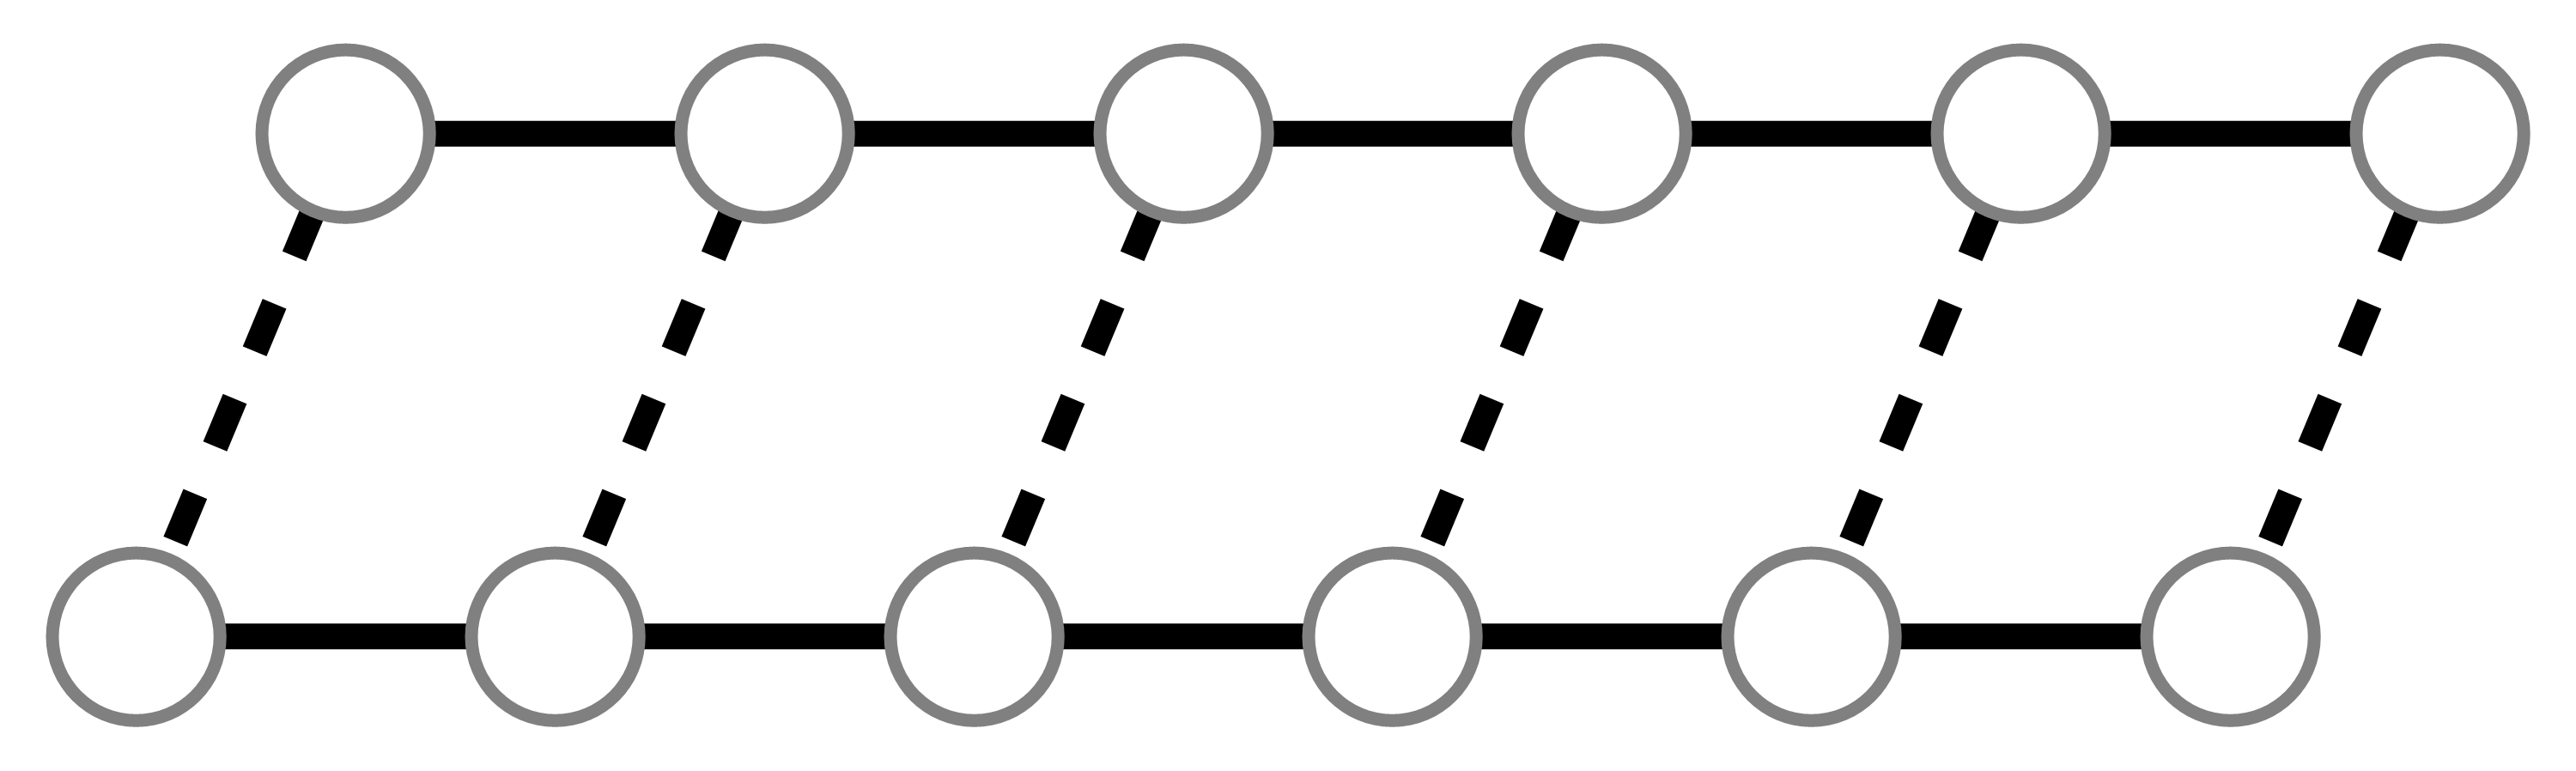
\includegraphics[scale=0.275]{Graphics/DNA_Model/dna_intact.pdf}
\caption{An intact DNA structure where $\{\mu\}=\{0,0,0,0,0,0\}$ for $N=6$.}
\label{fig:dna_intact}
\end{figure}
%
\subsection{Frayed DNA}

In a frayed configuration there is a single transfer matrix that links a broken base pair and an intact base pair, either $\hat{T}_{01}$ and $\hat{T}_{10}$. We have not considered the eigenvalue equation for this matrix but we can alter the way we contract the matrices, leaving the single matrix in one of the remaining integrals. Starting from \eqref{dna_z_eta} for $b$ broken base pairs the partition function looks like
%
\begin{align}
\label{dna_frayed_1}
Z\left(u\right)&=\sum_{s,t}\lambda_{s}^{N-1}\exp\left(-\frac{i4\pi s u}{L}\right)\int d\xi_{1}\,\psi_{s}\left(\xi_{1}\right)\exp\left(-\frac{V\left(\xi_{1}\right)}{2}\right)\hat{\psi}_{t}\left(\xi_{1}\right)\nonumber\\
&\times\int\prod_{j=1}^{N}d\eta_{j}\,\hat{T}_{00}\left(\eta_{1},\eta_{2}\right)...\hat{T}_{01}\left(\eta_{N-b-1},\eta_{N-b}\right)...\hat{T}_{11}\left(\eta_{N-1},\eta_{N}\right)\nonumber\\
&\times\hat{\psi}^{*}_{t}\left(\eta_{1}\right)\exp\left(-\frac{V\left(\eta_{N}\right)}{2}\right)\psi_{s}\left(\eta_{N}\right)
\end{align}
%
Similar to the intact state we can use the $\hat{\psi}^{*}_{t}\left(\eta_{1}\right)$ eigenfunction to contract the $\hat{T}_{00}$ transfer matrices up to $\eta_{N-b-1}$ to give 
%
\begin{align}
\label{dna_frayed_2}
Z\left(u\right)&=\sum_{s,t}\lambda_{s}^{N-1}\hat{\lambda}_{t}^{N-b}\exp\left(-\frac{i4\pi s u}{L}\right)\int d\xi_{1}\,\psi_{s}\left(\xi_{1}\right)\exp\left(-\frac{V\left(\xi_{1}\right)}{2}\right)\hat{\psi}_{t}\left(\xi_{1}\right)\nonumber\\
&\times\int\prod_{j=N-b-1}^{N}d\eta_{j}\,\hat{\psi}^{*}_{t}\left(\eta_{N-b-1}\right)\hat{T}_{01}\left(\eta_{N-b-1},\eta_{N-b}\right)...\hat{T}_{11}\left(\eta_{N-1},\eta_{N}\right)\nonumber\\
&\times\exp\left(-\frac{V\left(\eta_{N}\right)}{2}\right)\psi_{s}\left(\eta_{N}\right)
\end{align}
%
The eigenfunction $\psi_{s}\left(\eta_{N}\right)$ is unsuitable for contracting the remaining transfer matrices. To obtain an appropriate eigenfunction we expand $\psi_{s}\left(\eta_{N}\right)\exp\left(-\frac{V\left(\eta_{N}\right)}{2}\right)$ in the set of eigenfunctions of $\hat{T}_{11}$:
%
\begin{equation}
\psi_{s}\left(\eta_{N}\right)\exp\left(-\frac{V\left(\eta_{N}\right)}{2}\right) = \sum_{v}c^{s}_{v}\tilde{\psi}_{v}\left(\eta_{N}\right)
\end{equation}
%
where
%
\begin{equation}
c^{s}_{v}=\int d\eta'_{N}\,\psi_{s}\left(\eta'_{N}\right)\exp\left(-\frac{V\left(\eta'_{N}\right)}{2}\right)\tilde{\psi}^{*}_{v}\left(\eta'_{N}\right)
\end{equation}
%
Inserting these equations into \eqref{dna_frayed_2} we get 
%
\begin{align}
\label{dna_frayed_3}
Z\left(u\right)&=\sum_{s,t,v}\lambda_{s}^{N-1}\hat{\lambda}_{t}^{N-b}c^{s}_{v}\exp\left(-\frac{i4\pi s u}{L}\right)\int d\xi_{1}\,\psi_{s}\left(\xi_{1}\right)\exp\left(-\frac{V\left(\xi_{1}\right)}{2}\right)\hat{\psi}_{t}\left(\xi_{1}\right)\nonumber\\
&\times\int\prod_{j=N-b-1}^{N}d\eta_{j}\,\hat{\psi}^{*}_{t}\left(\eta_{N-b-1}\right)\hat{T}_{01}\left(\eta_{N-b-1},\eta_{N-b}\right)...\hat{T}_{11}\left(\eta_{N-1},\eta_{N}\right)\tilde{\psi}_{v}\left(\eta_{N}\right)
\end{align}
%
We are now able to contract the remaining transfer matrices using $\tilde{\psi}_{v}\left(\eta_{N}\right)$ and eigenvalue equation \eqref{dna_eign_twidle}. The residual transfer matrix $\hat{T}_{01}$ is left in the integral to be evaluated numerically. The expression for the partition function becomes
%
\begin{align}
\label{dna_frayed_4}
Z\left(u\right)&=\sum_{s,t,v}\lambda_{s}^{N-1}\hat{\lambda}_{t}^{N-b}\tilde{\lambda}_{v}^{b-1}c^{s}_{v}\exp\left(-\frac{i4\pi s u}{L}\right)\int d\xi_{1}\,\psi_{s}\left(\xi_{1}\right)\exp\left(-\frac{V\left(\xi_{1}\right)}{2}\right)\hat{\psi}_{t}\left(\xi_{1}\right)\nonumber\\
&\times\iint d\eta_{N-b-1}d\eta_{N-b}\,\hat{\psi}^{*}_{t}\left(\eta_{N-b-1}\right)\hat{T}_{01}\left(\eta_{N-b-1},\eta_{N-b}\right)\tilde{\psi}_{v}\left(\eta_{N-b}\right)
\end{align}
%
In the above equation the residual transfer matrix indicates that the broken base pairs lie on the right hand side of the structure as shown in \figref{dna_frayed}, but the symmetric nature of the structure means that this equation would give the same results for broken base pairs from left side of the ladder structure.
%
\subsection{Double Frayed DNA}

The symmetric behaviour of the system suggests that the base pairs corresponding to $\eta_1$ and $\eta_N$ should break at the same time. With the remaining base pairs intact we can consider this as a double frayed state such that base pairs break at both ends of the ladder structure. Using $b$ and $b'$ to denote the number of broken base pairs at each end we employ a different expansion of the delta function boundary conditions where
%
\begin{align}
\label{df_dna_delta_1}
\delta\left(\xi_{1}-\eta_{1}\right)&=\sum_{v}\tilde{\psi}_{v}\left(\xi_{1}\right)\tilde{\psi}^{*}_{v}\left(\eta_{1}\right)\\
\label{df_dna_delta_2}
\delta\left(\xi_{N}+\eta_{N}-2u\right)&=\sum_{s}\psi^{*}_{s}\left(2u-\xi_{N}\right)\psi_{s}\left(\eta_{N}\right)
\end{align}
%
Using eigenfunctions of the $\hat{T}_{11}$ transfer matrices, the contractions of the $T$ transfer matrices are not affected by this new expansion. The partition function integral becomes
%
\begin{align}
\label{dna_dfray_1}
Z&\left(u\right)=\sum_{s,v}\lambda_{s}^{N-1}\exp\left(-\frac{4\pi isu}{L}\right)\int d\xi_{1}\,\psi_{s}\left(\xi_{1}\right)\exp\left(-\frac{V\left(\xi_{1}\right)}{2}\right)\tilde{\psi}_{v}\left(\xi_{1}\right)\int\prod_{j=1}^{N}d\eta_{j}\nonumber\\
&\times\psi_{s}\left(\eta_{N}\right)\exp\left(-\frac{V\left(\eta_{N}\right)}{2}\right)\tilde{\psi}^{*}_{v}\left(\eta_{1}\right)\hat{T}_{11}\left(\eta_{1},\eta_{2}\right)...\hat{T}_{10}\left(\eta_{b},\eta_{b+1}\right)\hat{T}_{00}\left(\eta_{b+1},\eta_{b+2}\right)...\nonumber\\
&...\hat{T}_{00}\left(\eta_{N-b'-2},\eta_{N-b'-1}\right)\hat{T}_{01}\left(\eta_{N-b'},\eta_{N-b'+1}\right)...\hat{T}_{11}\left(\eta_{N-1},\eta_{N}\right)
\end{align}
%
We make an expansion of the functions in $\eta_N$ in terms of eigenfunctions of the $\hat{T}_{11}$ transfer matrix:
%
\begin{equation}
\psi_{s}\left(\eta_{N}\right)\exp\left(-\frac{V\left(\eta_{N}\right)}{2}\right) = \sum_{v'}D^{s}_{v'}\tilde{\psi}_{v'}\left(\eta_{N}\right)
\end{equation}
%
where
%
\begin{equation}
\label{dna_d1_matrix}
D^{s}_{v'}=\int d\eta'_{N}\,\psi_{s}\left(\eta'_{N}\right)\exp\left(-\frac{V\left(\eta'_{N}\right)}{2}\right)\tilde{\psi}^{*}_{v'}\left(\eta'_{N}\right)
\end{equation}
%
Inserting this expression into the partition function we get
%
\begin{align}
\label{dna_dfray_2}
Z\left(u\right)&=\sum_{s,v,v'}\lambda_{s}^{N-1}D^{s}_{v'}\exp\left(-\frac{4\pi isu}{L}\right)\int d\xi_{1}\,\psi_{s}\left(\xi_{1}\right)\exp\left(-\frac{V\left(\xi_{1}\right)}{2}\right)\tilde{\psi}_{v}\left(\xi_{1}\right)\nonumber\\
&\times\int\prod_{j=1}^{N}d\eta_{j}\,\tilde{\psi}^{*}_{v}\left(\eta_{1}\right)\hat{T}_{11}\left(\eta_{1},\eta_{2}\right)...\hat{T}_{10}\left(\eta_{b},\eta_{b+1}\right)\hat{T}_{00}\left(\eta_{b+1},\eta_{b+2}\right)...\nonumber\\
&...\hat{T}_{00}\left(\eta_{N-b'-2},\eta_{N-b'-1}\right)\hat{T}_{01}\left(\eta_{N-b'},\eta_{N-b'+1}\right)...\hat{T}_{11}\left(\eta_{N-1},\eta_{N}\right)\tilde{\psi}_{v'}\left(\eta_{N}\right)
\end{align}
%
After making the relevant contractions using the properties of the $\tilde{\psi}_{v}$ and $\tilde{\psi}_{v'}$ eigenfunctions we get
%
\begin{align}
\label{dna_dfray_3}
Z\left(u\right)&=\sum_{s,v,v'}\lambda_{s}^{N-1}\tilde{\lambda}_{v}^{b-1}\tilde{\lambda}_{v'}^{b'-1}D^{s}_{v'}\exp\left(-\frac{4\pi isu}{L}\right)\int d\xi_{1}\,\psi_{s}\left(\xi_{1}\right)\exp\left(-\frac{V\left(\xi_{1}\right)}{2}\right)\tilde{\psi}_{v}\left(\xi_{1}\right)\nonumber\\
&\times\int\prod_{j=b}^{N-b'+1}d\eta_{j}\,\tilde{\psi}^{*}_{v}\left(\eta_{b}\right)\hat{T}_{10}\left(\eta_{b},\eta_{b+1}\right)\hat{T}_{00}\left(\eta_{b+1},\eta_{b+2}\right)...\nonumber\\
&...\hat{T}_{00}\left(\eta_{N-b'-2},\eta_{N-b'-1}\right)\hat{T}_{01}\left(\eta_{N-b'},\eta_{N-b'+1}\right)\tilde{\psi}_{v'}\left(\eta_{N-b'+1}\right)
\end{align}
%
To contract the remaining $\hat{T}_{00}$ transfer matrices we introduce a pair of appropriate eigenfunctions by inserting the following representation of unity:
%
\begin{equation}
\int_{-\infty}^{\infty}\delta\left(\phi-\eta_{N-b'}\right)d\phi=\int_{-\infty}^{\infty}d\phi\sum_{t}\hat{\psi}_{t}\left(\phi\right)\hat{\psi}_{t}^{*}\left(\eta_{N-b'}\right)
\end{equation}
%
where $\phi$ is a dummy variable. After further contractions the partition function becomes
%
\begin{align}
\label{dna_dfray_4}
Z\left(u\right)&=\sum_{s,v,v',t}\lambda_{s}^{N-1}\tilde{\lambda}_{v}^{b-1}\tilde{\lambda}_{v'}^{b'-1}\hat{\lambda}_{t}^{N-b-b'-1}D^{s}_{v'}\exp\left(-\frac{4\pi isu}{L}\right)\nonumber\\
&\times\int d\xi_{1}\,\psi_{s}\left(\xi_{1}\right)\exp\left(-\frac{V\left(\xi_{1}\right)}{2}\right)\tilde{\psi}_{v}\left(\xi_{1}\right)\iint d\eta_{b}\,d\phi\,\tilde{\psi}^{*}_{v}\left(\eta_{b}\right)\hat{T}_{10}\left(\eta_{b},\phi\right)\hat{\psi}_{t}\left(\phi\right)\nonumber\\
&\times\iint d\eta_{N-b'}\,d\eta_{N-b'+1}\,\hat{\psi}_{t}^{*}\left(\eta_{N-b'}\right)\hat{T}_{01}\left(\eta_{N-b'},\eta_{N-b'+1}\right)\tilde{\psi}_{v'}\left(\eta_{N-b'+1}\right)
\end{align}
%
The remaining expression involves five integrals and four summations.

\subsection{Bubbling DNA}
%
Bubbling in dsDNA occurs when broken base pairs exist within the structure, not at the ends. This requires us to consider two regions of the ladder structure that have intact base pairs and a region in the middle with broken base pairs. If we consider a configuration where we have $l$ intact base pairs followed by $b$ broken base pairs with the remaining base pairs intact such that $l+b<N$, the partition function integral would be of the form
%
\begin{align}
\label{dna_bubble_1}
Z&\left(u\right)=\sum_{s,t}\lambda_{s}^{N-1}\exp\left(-\frac{4\pi isu}{L}\right)\int d\xi_{N}\,\psi_{s}\left(\xi_{N}\right)\exp\left(-\frac{V\left(\xi_{N}\right)}{2}\right)\hat{\psi}^{*}_{t}\left(\xi_{N}\right)\int\prod_{j=1}^{N}d\eta_{j}\nonumber\\
&\times\psi_{s}\left(\eta_{N}\right)\exp\left(-\frac{V\left(\eta_{N}\right)}{2}\right)\hat{\psi}^{*}_{t}\left(\eta_{1}\right)\hat{T}_{00}\left(\eta_{1},\eta_{2}\right)...\hat{T}_{00}\left(\eta_{l-1},\eta_{l}\right)\hat{T}_{01}\left(\eta_{l},\eta_{l+1}\right)\hat{T}_{11}\left(\eta_{l+1},\eta_{l+2}\right)...\nonumber\\
&...\hat{T}_{11}\left(\eta_{l+b-1},\eta_{l+b}\right)\hat{T}_{10}\left(\eta_{l+b},\eta_{l+b+1}\right)\hat{T}_{00}\left(\eta_{l+b+1},\eta_{l+b+2}\right)...\hat{T}_{00}\left(\eta_{N-1},\eta_{N}\right)
\end{align}
%
The eigenfunction $\hat{\psi}^{*}_{t}$ is available to contract the transfer matrices for intact base pairs from $\eta_{1}\to \eta_{l}$. However, for the transfer matrices from $\eta_{N} \to \eta_{l+b+1}$ we need to expand $\psi_{s}\left(\eta_{N}\right)\exp\left(-\frac{V\left(\eta_{N}\right)}{2}\right)$ in the set of eigenfunctions of $\hat{T}_{00}$,
%
\begin{equation}
\psi_{s}\left(\eta_{N}\right)\exp\left(-\frac{V\left(\eta_{N}\right)}{2}\right) = \sum_{t'}d^{s}_{t'}\hat{\psi}_{t'}\left(\eta_{N}\right)
\end{equation}
%
where
%
\begin{equation}
\label{dna_d_matrix}
d^{s}_{t'}=\int d\eta'_{N}\,\psi_{s}\left(\eta'_{N}\right)\exp\left(-\frac{V\left(\eta'_{N}\right)}{2}\right)\hat{\psi^{*}_{t'}}\left(\eta'_{N}\right)
\end{equation}
%
By inserting these expressions into \eqref{dna_bubble_1} we can contract all the $\hat{T}_{00}$ transfer matrices to give
%
\begin{align}
\label{dna_bubble_2}
Z\left(u\right)&=\sum_{s,t,t'}\lambda_{s}^{N-1}\hat{\lambda}_{t}^{l-1}\hat{\lambda}_{t'}^{N-l-b-1}d^{s}_{t'}\exp\left(-\frac{4\pi isu}{L}\right)\int d\xi_{N}\,\psi_{s}\left(\xi_{N}\right)\exp\left(-\frac{V\left(\xi_{N}\right)}{2}\right)\hat{\psi}^{*}_{t}\left(\xi_{N}\right)\nonumber\\
&\times\int\prod_{j=l}^{N-l-b}d\eta_{j}\hat{\psi}^{*}_{t}\left(\eta_{l}\right)\hat{T}_{01}\left(\eta_{l},\eta_{l+1}\right)\hat{T}_{11}\left(\eta_{l+1},\eta_{l+2}\right)...\hat{T}_{11}\left(\eta_{l+b-1},\eta_{l+b}\right)...\nonumber\\
&\times\hat{T}_{10}\left(\eta_{l+b},\eta_{l+b+1}\right)\hat{\psi}_{t'}\left(\eta_{l+b+1}\right)
\end{align}
%
To contract the remaining $\hat{T}_{11}$ transfer matrices we introduce a pair of appropriate eigenfunctions by inserting the following representation of unity:
%
\begin{equation}
\int_{-\infty}^{\infty}\delta\left(\phi-\eta_{l+b}\right)d\phi=\int_{-\infty}^{\infty}d\phi\sum_{v}\tilde{\psi^{*}_{v}}\left(\phi\right)\tilde{\psi_{v}}\left(\eta_{l+b}\right)
\end{equation}
%
where $\phi$ is a dummy variable. After the final contractions the partition function becomes
%
\begin{align}
Z&\left(u\right)=\sum_{s,t,t',v}\lambda_{s}^{N-1}\hat{\lambda}_{t}^{l-1}\hat{\lambda}_{t'}^{N-l-b-1}\tilde{\lambda}_{v}^{b-1}d^{s}_{t'}\exp\left(-\frac{4\pi isu}{L}\right)\nonumber\\
&\times\int d\xi_{N}\,\psi_{s}\left(\xi_{N}\right)\exp\left(-\frac{V\left(\xi_{N}\right)}{2}\right)\hat{\psi}^{*}_{t}\left(\xi_{N}\right)\nonumber\\
&\times\int d\eta_{l}\int d\phi\,\hat{\psi}_{t'}\left(\eta_{l}\right)\hat{T}_{01}\left(\eta_{l},\phi\right)\tilde{\psi^{*}_{v}}\left(\phi\right)\nonumber\\
&\times\int d\eta_{l+b}\int d\eta_{l+b+1}\,\tilde{\psi_{v}}\left(\eta_{l+b}\right)\hat{T}_{10}\left(\eta_{l+b},\eta_{l+b+1}\right)\hat{\psi}_{t}\left(\eta_{l+b+1}\right)
\end{align}
%
once again involving five integrations and four summations.
%
\section{Mean Axial Displacement}
%
We now employ the partition function to determine mean axial displacement patterns for various patterns of breakage. Increasing the extension $u$ in the DNA ladder structure increases the stress across each of the base pairs. The redistribution of the forces in the ladder structure means that the mean axial displacement for each base pair will not be the same. We can calculate the average of the structural variables $\xi$ and $\eta$ from the knowledge of the partition function. These mean axial displacements with the boundary conditions labelled as $C\left(u\right)$ are
%
\begin{equation}
\label{dna_mxd_xi}
\langle\xi_{\alpha}\rangle=\frac{\int \prod^{N}_{j=1}d\xi_{j}d\eta_{j}\,\xi_{\alpha}\exp\left(-\beta H\left(\xi_{j},\eta_{j}\right)\right)C\left(u\right)}{\int \prod^{N}_{j=1}d\xi_{j}d\eta_{j}\,\exp\left(-\beta H\left(\xi_{j},\eta_{j}\right)\right)C\left(u\right)}
\end{equation}
%
\begin{equation}
\label{dna_mxd_eta}
\langle\eta_{\alpha}\rangle=\frac{\int \prod^{N}_{j=1}d\xi_{j}d\eta_{j}\,\eta_{\alpha}\exp\left(-\beta H\left(\xi_{j},\eta_{j}\right)\right)C\left(u\right)}{\int \prod^{N}_{j=1}d\xi_{j}d\eta_{j}\,\exp\left(-\beta H\left(\xi_{j},\eta_{j}\right)\right)C\left(u\right)}
\end{equation}
%
where the denominator is the partition function \eqref{dna_partition_function}. Recombining these quantities using \eqref{dna_transform_xi} and \eqref{dna_transform_eta} we are able to find the average positions $\langle x_{\alpha}\rangle$ and $\langle y_{\alpha}\rangle$.

\subsection{Calculation of average $\eta_{\alpha}$}

In the intact state of DNA the calculation of average $\eta_{\alpha}$ requires the evaluation of the following integral using the transfer integral method
%
\begin{equation}
Z_{\eta_{\alpha}}\left(u\right)=\int \prod^{N}_{j=1}d\xi_{j}d\eta_{j}\,\eta_{\alpha}\exp\left(-\beta H\left(\xi_{j},\eta_{j}\right)\right)C\left(u\right)
\end{equation}
%
This integral only affects the contraction of transfer matrices in $\eta$, therefore we can continue from a modified version of \eqref{dna_z_eta} that includes $\eta_{\alpha}$
%
\begin{align}
\label{dna_mxd_z_eta}
Z_{\eta_{\alpha}}\left(u\right)&=\sum_{s,t}\lambda_{s}^{N-1}\exp\left(-\frac{4\pi isu}{L}\right)\int d\xi_{N}\,\psi_{s}\left(\xi_{N}\right)\exp\left(-\frac{V\left(\xi_{N}\right)}{2}\right)\hat{\psi}^{*}_{t}\left(\xi_{N}\right)\nonumber\\
&\times\int\prod_{j=1}^{N}d\eta_{j}\,\psi_{s}\left(\eta_{N}\right)\exp\left(-\frac{V\left(\eta_{N}\right)}{2}\right)\hat{\psi}_{t}^{*}\left(\eta_{1}\right)\eta_{\alpha}\left(\prod_{j'=1}^{N-1}\hat{T}_{\mu_{j'},\mu_{j'+1}}\left(\eta_{j'+1},\eta_{j'}\right)\right)
\end{align}
%
Setting $\mu=0$ for all the base pairs we are left with $\eta_{\alpha}$ within a set of transfer matrices. For a given $\eta_{\alpha}$ the partition function becomes
%
\begin{align}
\label{dna_mxd_z_eta2}
Z_{\eta_{\alpha}}\left(u\right)&=\sum_{s,t}\lambda_{s}^{N-1}\exp\left(-\frac{4\pi isu}{L}\right)\int d\xi_{N}\,\psi_{s}\left(\xi_{N}\right)\exp\left(-\frac{V\left(\xi_{N}\right)}{2}\right)\hat{\psi}^{*}_{t}\left(\xi_{N}\right)\nonumber\\
&\times\int\prod_{j=1}^{N}d\eta_{j}\,\psi_{s}\left(\eta_{N}\right)\exp\left(-\frac{V\left(\eta_{N}\right)}{2}\right)\hat{\psi}_{t}^{*}\left(\eta_{1}\right)\nonumber\\
&\times\hat{T}_{00}\left(\eta_{1},\eta_{2}\right)....\hat{T}_{00}\left(\eta_{\alpha-1},\eta_{\alpha}\right)\eta_{\alpha}\hat{T}_{00}\left(\eta_{\alpha},\eta_{\alpha+1}\right)...\hat{T}_{00}\left(\eta_{N-1},\eta_{N}\right)
\end{align}
%
We now contract the matrices using the relevant eigenvalue equations starting from $\eta_{1}$, and downwards from $\eta_{N}$, leaving $\eta_{\alpha}$ left in the integral. 
%
\begin{align}
\label{dna_mxd_z_eta3}
Z_{\eta_{\alpha}}\left(u\right)&=\sum_{s,t,t'}\lambda_{s}^{N-1}\hat{\lambda}_{t}^{\alpha-1}\hat{\lambda}_{t'}^{N-\alpha}d^{s}_{t'}\exp\left(-\frac{i4\pi s u}{L}\right)\nonumber\\
&\times\int d\xi_{1}\,\psi_{s}\left(\xi_{1}\right)\exp\left(-\frac{V\left(\xi_{1}\right)}{2}\right)\hat{\psi}_{t}\left(\xi_{1}\right)\int d\eta_{\alpha}\, \hat{\psi}^{*}_{t}\left(\eta_{\alpha}\right)\eta_{\alpha}\hat{\psi}_{t'}\left(\eta_{\alpha}\right)
\end{align}
%
where $d^{s}_{t'}$ is given by \eqref{dna_d_matrix}.

\subsection{Calculation of average $\xi_{\alpha}$}

To calculate the $Z_{\xi_{\alpha}}$ integral we begin from a modified version of \eqref{dna_z_eta} that includes the extra term $\xi_{\alpha}$ and use $\hat{\psi_{t}^{*}}\left(\eta_{1}\right)$ to contract all the $\hat{T}$ transfer matrices up to $\eta_{N}$
%
\begin{align}
Z_{\xi_{\alpha}}\left(u\right)&=\sum_{s,t}\hat{\lambda}_{t}^{N-1}\exp\left(-\frac{i4\pi s u}{L}\right)\\
&\times\int d\eta_{N}\,\psi_{s}\left(\eta_{N}\right)\exp\left(-\frac{V\left(\eta_{N}\right)}{2}\right)\hat{\psi}^{*}_{t}\left(\eta_{N}\right)\nonumber\\
&\times\int \prod_{i=1}^{N}d\xi_{i}\,\left(\prod_{i'=1}^{N-1}T\left(\xi_{i'+1},\xi_{i'}\right)\right)\xi_{\alpha}\hat{\psi}_{t}\left(\xi_{1}\right)\psi_{s}\left(\xi_{N}\right)\exp\left(-\frac{V\left(\xi_{1}\right)}{2}\right)\nonumber
\end{align}
%
We then use $\psi_{s}$ to contract the first set of $T$ transfer matrices from $\xi_{N}$ down to $\xi_{\alpha}$
%
\begin{align}
Z_{\xi_{\alpha}}\left(u\right)&=\sum_{s,t}\lambda_{s}^{N-\alpha}\hat{\lambda}_{t}^{N-1}\exp\left(-\frac{i4\pi s u}{L}\right)\\
&\times\int d\eta_{N}\,\psi_{s}\left(\eta_{N}\right)\exp\left(-\frac{V\left(\eta_{N}\right)}{2}\right)\hat{\psi}^{*}_{t}\left(\eta_{N}\right)\nonumber\\
&\times\int \prod_{i=1}^{\alpha}d\xi_{i}\,\left(\prod_{i'=1}^{\alpha-1}T\left(\xi_{i'+1},\xi_{i'}\right)\right)\psi_{s}\left(\xi_{\alpha}\right)\xi_{\alpha}\hat{\psi}_{t}\left(\xi_{1}\right)\exp\left(-\frac{V\left(\xi_{1}\right)}{2}\right)\nonumber
\end{align}
%
To contract the remaining set of transfer matrices we perform an expansion of the $\hat{\psi}_t$ eigenfunction in $\psi_{s}$
%
\begin{equation}
\hat{\psi}_{t}\left(\xi_{1}\right)\exp\left(-\frac{V\left(\xi_{1}\right)}{2}\right) = \sum_{s'}h^{t}_{s'}\psi_{s'}\left(\xi_{1}\right)
\end{equation}
%
where
%
\begin{equation}
\label{dna_h_matrix}
h^{t}_{s'}=\int d\xi'_{1}\,\psi^{*}_{s'}\left(\xi'_{1}\right)\exp\left(-\frac{V\left(\xi'_{1}\right)}{2}\right)\hat{\psi_{t}}\left(\xi'_{1}\right)
\end{equation}
%
Inserting this into the partition function we are now able to contract the remaining $T$ transfer matrices to get
%
\begin{align}
Z_{\xi_{\alpha}}\left(u\right)&=\sum_{s,s',t}\lambda_{s'}^{\alpha-1}\lambda_{s}^{N-\alpha}\hat{\lambda}_{t}^{N-1}\exp\left(-\frac{i4\pi s u}{L}\right)h^{t}_{s'}\nonumber\\
&\times\int d\eta_{N}\,\psi_{s}\left(\eta_{N}\right)\exp\left(-\frac{V\left(\eta_{N}\right)}{2}\right)\hat{\psi}^{*}_{t}\left(\eta_{N}\right)\int d\xi_{\alpha}\, \psi_{s'}\left(\xi_{\alpha}\right)\xi_{\alpha}\psi_{s}\left(\xi_{\alpha}\right)
\end{align}
%
Next we perform numerical calculations using these expressions.

\section{Results for DNA eigensystem calculations}

The numerical calculation of the eigenvalue problem was discretised into $2m+1$ steps over an interval range $\left[-\frac{L}{2},\frac{L}{2}\right]$ to give a step size $\Delta = \frac{L}{2m+1}$. The accuracy of the eigenvalue calculations is dependent on the $L$ and $m$ variables and the associated determination of $\Delta$ in the numerical calculation. There is a balance to be found between the discretisation of the eigenvalue problem, and the range in $\eta$ that can be included in the integrals. For the $T$ and $\hat{T}$ transfer matrices in the DNA model, and for a given $\Delta$, we sampled a variety of different $L$ and $m$ combinations in order to determine their effect on the accuracy of the numerical calculations. The eigenvalues for $\lambda_s$ are shown in Figs.~\ref{fig:dna_eval_s}-\ref{fig:dna_eval_s3} for a range of $\Delta$, and the $\hat{\lambda}_t$ eigenvalues that correspond to the Parisi eigenvalues of the $\hat{T}$ transfer matrix where $\eta_B =L/2$ are shown in Figs.~\ref{fig:dna_eval_t00_delta0.25}-\ref{fig:dna_eval_t00_delta0.5}.

Analysis of the $\lambda_s$ eigenvalues of the $T$ transfer matrix indicates that it is possible to find a combination of $L$ and $m$ that produces sufficient agreement between numerical and analytical values for all $\Delta$. From the results shown in \figref{dna_eval_s_50_50}, \figref{dna_eval_s_50_100}, and \figref{dna_eval_s_50_250} we are able to observe that this is brought about by increasing the integral range parameter $L$. Another example of this effect can be seen by comparing the results in \figref{dna_eval_s_5_10}, and \figref{dna_eval_s_10_10}. Both these plots have $m=10$ and we note that as we increase $L$ from 5 to 10 we find the agreement between the analytical and numerical results improves. Expecting the increase of $L$ to have the same effect on the $\hat{\lambda}_t$ eigenvalues of the $\hat{T}$ transfer matrix, we discover that for all combinations of $L$ and $m$ there are excellent agreements between the numerical and analytical calculations as shown in \figref{dna_eval_t00_delta0.25} and \figref{dna_eval_t00_delta0.5}. 

The eigenfunction plots of $\hat{\psi}_t$ in \figref{nVa_dna_psi_t00_delta0.5}, and \figref{nVa_dna_psi_t00_delta0.25} for the highest eigenvalues corresponding to $t=1,2,3,4$ show that every eigenfunction has a limited range in $\eta$, and therefore by choosing a small $L$ we are able to capture the non-zero parts of the integral equation \eqref{dna_eign_hat} when calculating the eigenvalues. The eigenfunctions for $\psi_s$ are periodic and therefore do not contain this limited range in $\eta$. 

\begin{comment}
Eigenfunctions for $\psi_s$ do not have this limited range in $\eta$ where $\hat{\psi}_s(\eta) =0$ for $\eta \ll \frac{L}{2}$. The range of these eigenfunctions exist up to $\eta=\frac{L}{2}$.
\end{comment}

The eigenfunctions in \figref{nVa_dna_psi_t00_delta0.5}, and \figref{nVa_dna_psi_t00_delta0.25} also demonstrate that by reducing $\Delta$ we increase the resolution of the numerically generated eigenfunctions. This is essential for an accurate free energy calculation by numerical methods as it increases the number of data points in the discrete representation of the eigenfunction.

Turning our attention to the eigenfunctions $\hat{\psi}$ and $\tilde{\psi}$ of the $\hat{T}_{00}$ and $\hat{T}_{11}$ transfer matrices, respectively, we are able to observe the effect of finite $\eta_B$ on the eigenfunctions through the $g$ factors we imposed in \eqref{dna_g0}, and \eqref{dna_g1} . The eigenfunction $\hat{\psi}_t$ shown in \figref{dna_psi_t00_delta0.25} is non-zero only for $|\eta | \leq \eta_{B}$ and the opposite behaviour of the $\tilde{\psi}_t$ eigenfunction is shown in \figref{dna_psi_t11_delta0.25}.

\subsection{Conclusion}

Analysis of the eigenvalue calculations gives an insight into the range of parameters that would be suitable to perform partition function calculations. We have found that a balance of choosing $L$ and $m$ is needed in order to perform integrations over a suitable range, as well as providing enough data points within the eigenfunction to calculate the partition function accurately.

The plots for both the eigenvalues and eigenvectors of the $T$ and $\hat{T}$ transfer matrices have a high degree of accuracy when we compare the numerical and analytical results. For the eigenvalues of $\lambda_s$, the plots converge to a perfect fit as $L$ is increased to 50, and from all the plots we find that by having a sufficient integral range over $\eta$ we can encapsulate the complete eigenfunction. Considering the discretisation parameters we have used, the results are accurate when $L$ is chosen in the range of 25 to 50, and $m$ in a range of 50 to 100. 

It is possible to increase the accuracy of the eigenvalues and eigenfunctions further by choosing larger discretisation parameters, however, as we can see in \figref{dna_eval_s_50_250} this effect is minimal if we compare it to \figref{dna_eval_s_25_125}. A disadvantage of increasing $m$ is that it results in a significant increase in computation time.

%%% Eigenvalue T %%%
\begin{figure}[H]
\centering
\begin{tabular}{cc}
\subfloat[$L=5$ $m=5$]{\label{fig:dna_eval_s_5_5}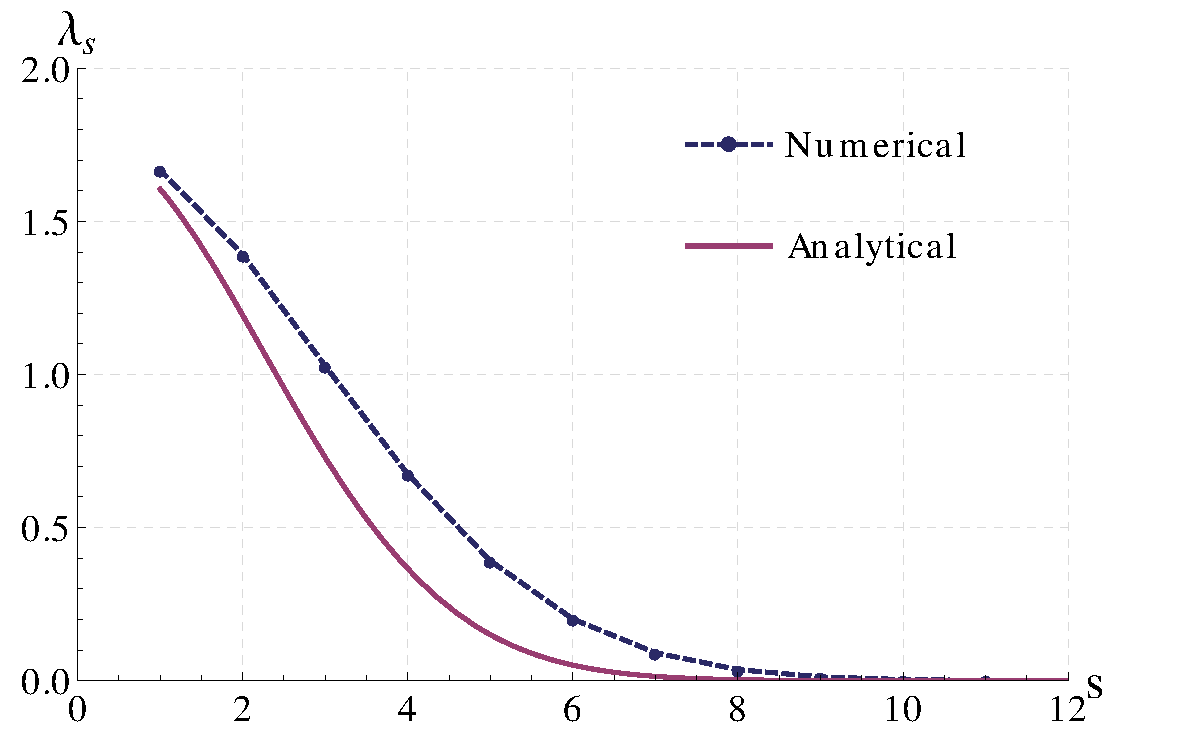
\includegraphics[scale=0.325]{Results/DNA/Eigensystem/T/0.5/lambda_s_L5_m5.pdf}} &
\subfloat[$L=10$ $m=10$]{\label{fig:dna_eval_s_10_10}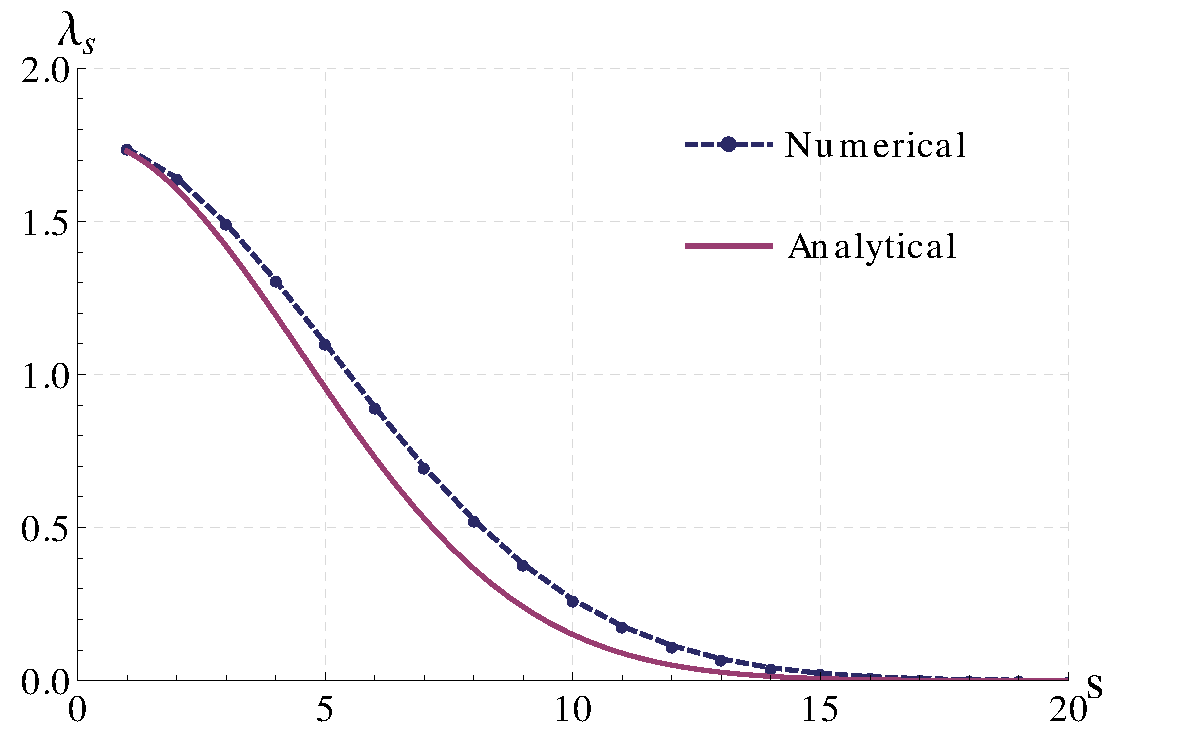
\includegraphics[scale=0.325]{Results/DNA/Eigensystem/T/0.5/lambda_s_L10_m10.pdf}} \\
\subfloat[$L=25$ $m=25$]{\label{fig:dna_eval_s_25_25}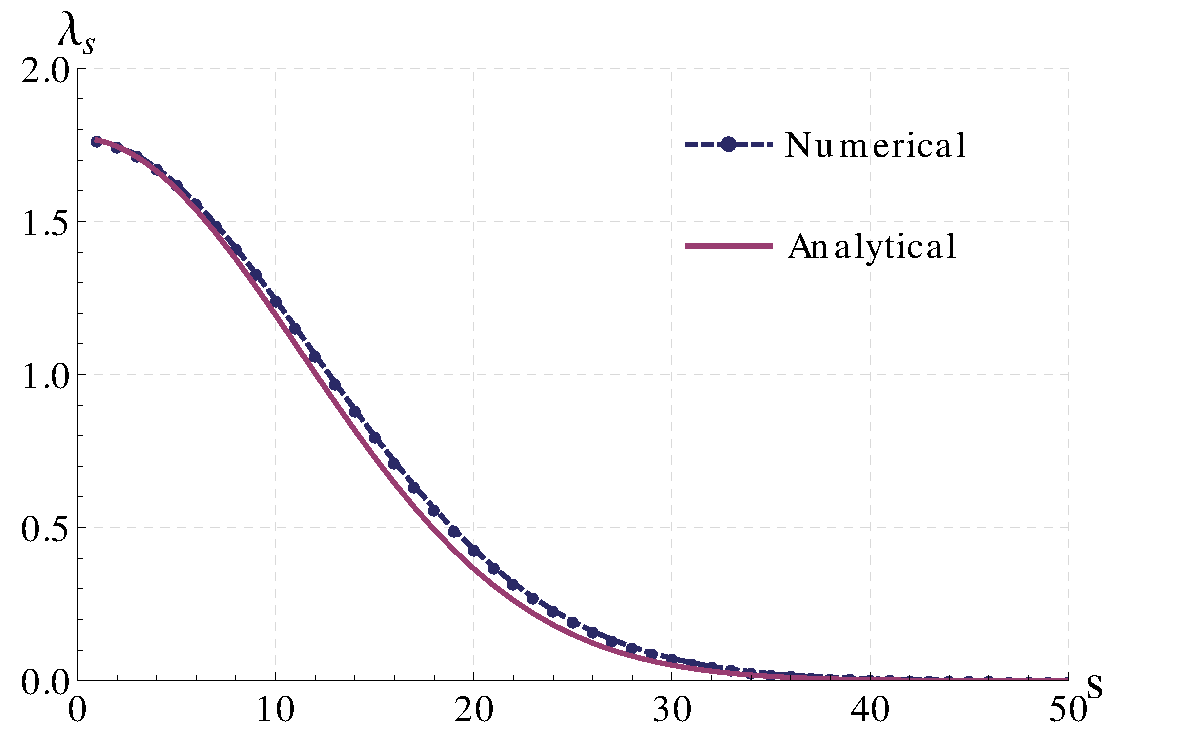
\includegraphics[scale=0.325]{Results/DNA/Eigensystem/T/0.5/lambda_s_L25_m25.pdf}} &
\subfloat[$L=50$ $m=50$]{\label{fig:dna_eval_s_50_50}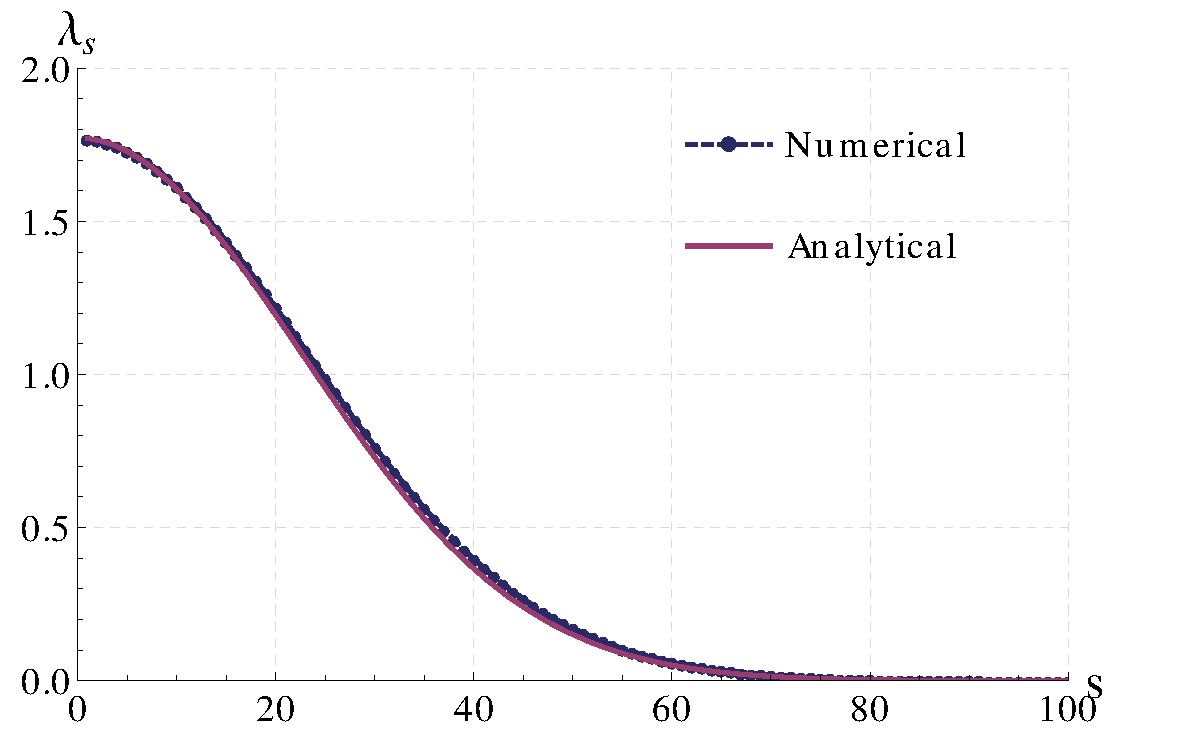
\includegraphics[scale=0.325]{Results/DNA/Eigensystem/T/0.5/lambda_s_L50_m50.pdf}}
\end{tabular}
\caption{Numerical and analytical eigenvalue plots for $\lambda_{s}$ where the $2m+1$ eigenvalues are shown in descending order. Different combinations of $L$ and $m$ are used such that $\Delta=0.5$ in these calculations.}
\label{fig:dna_eval_s} 
\end{figure}

\begin{figure}[H]
\centering
\begin{tabular}{cc}
\subfloat[$L=5$ $m=10$]{\label{fig:dna_eval_s_5_10}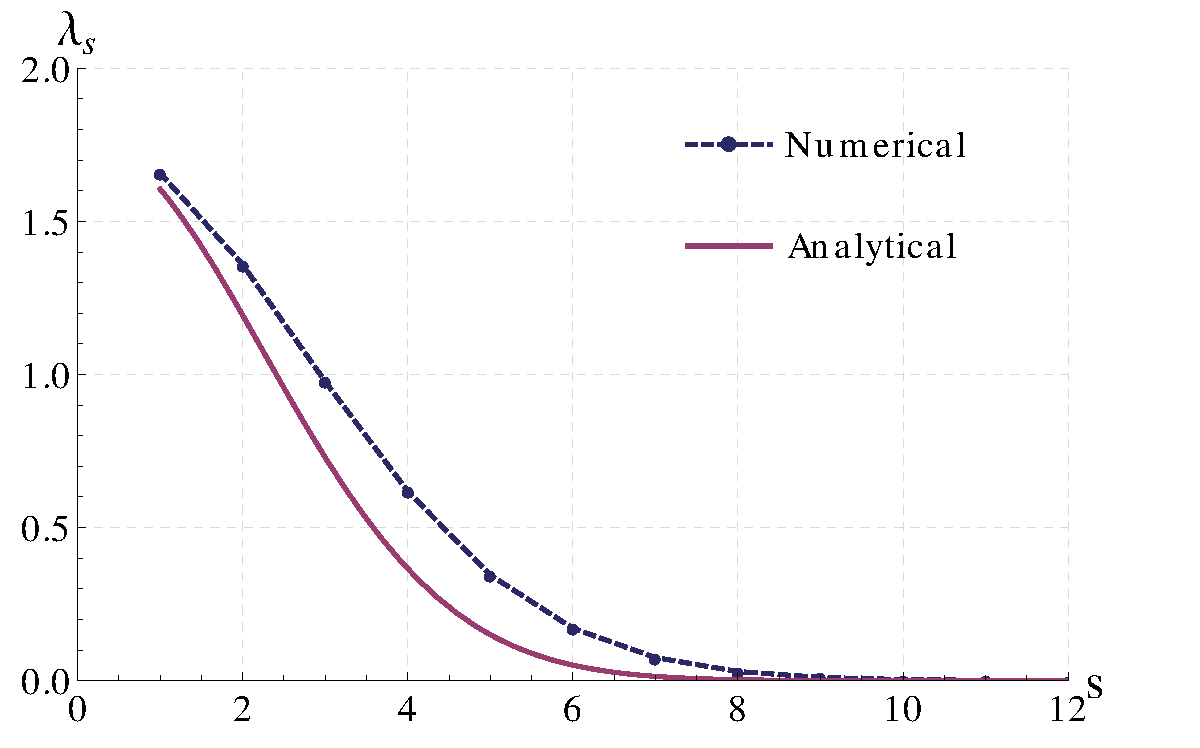
\includegraphics[scale=0.325]{Results/DNA/Eigensystem/T/0.25/lambda_s_L5_m10.pdf}} &
\subfloat[$L=10$ $m=20$]{\label{fig:dna_eval_s_10_20}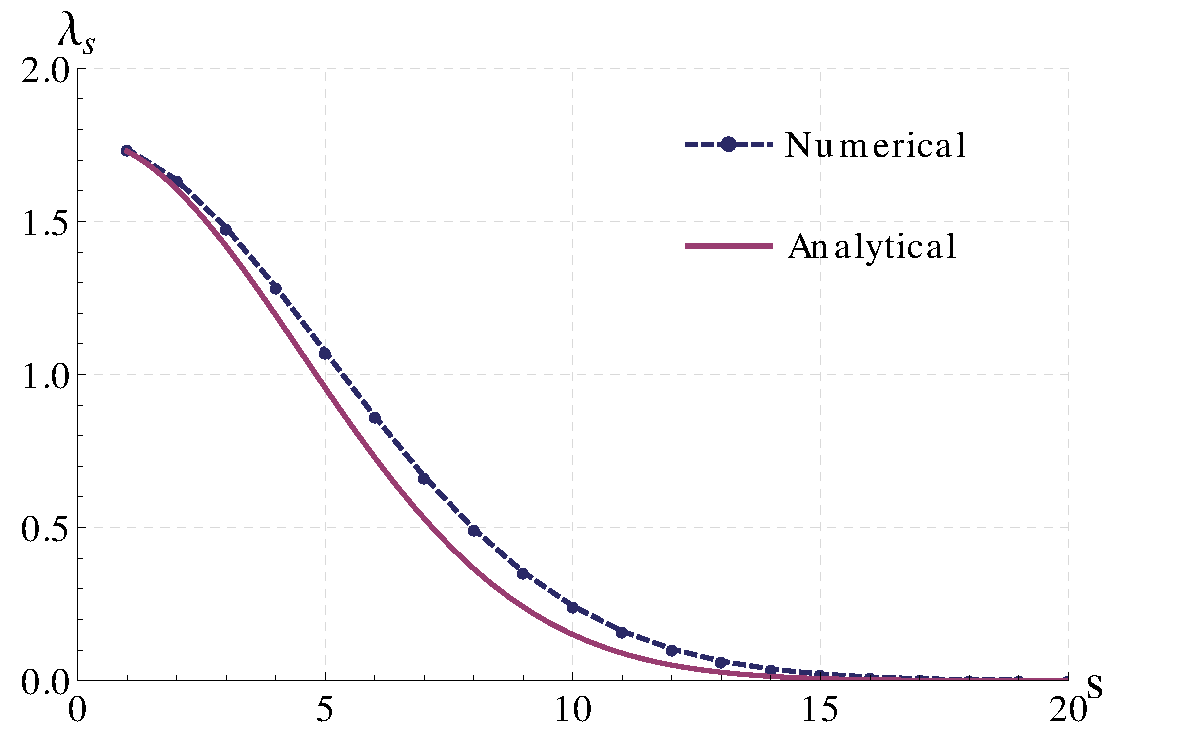
\includegraphics[scale=0.325]{Results/DNA/Eigensystem/T/0.25/lambda_s_L10_m20.pdf}} \\
\subfloat[$L=25$ $m=50$]{\label{fig:dna_eval_s_25_50}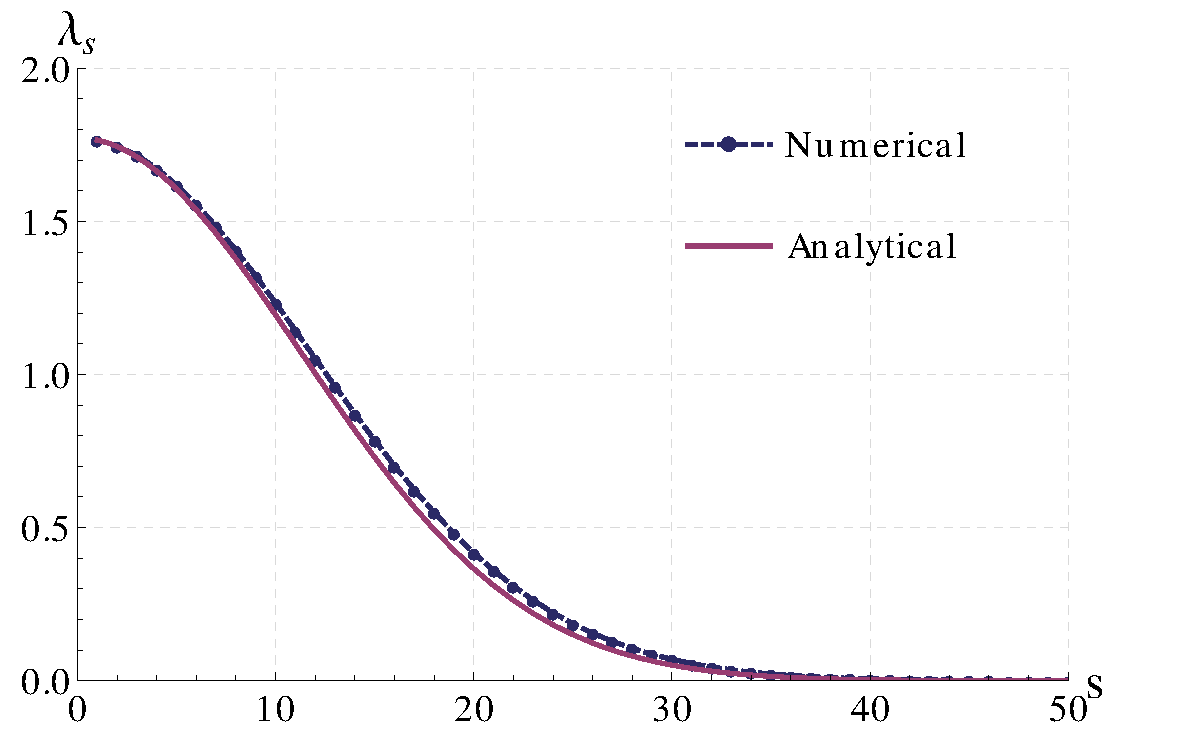
\includegraphics[scale=0.325]{Results/DNA/Eigensystem/T/0.25/lambda_s_L25_m50.pdf}} &
\subfloat[$L=50$ $m=100$]{\label{fig:dna_eval_s_50_100}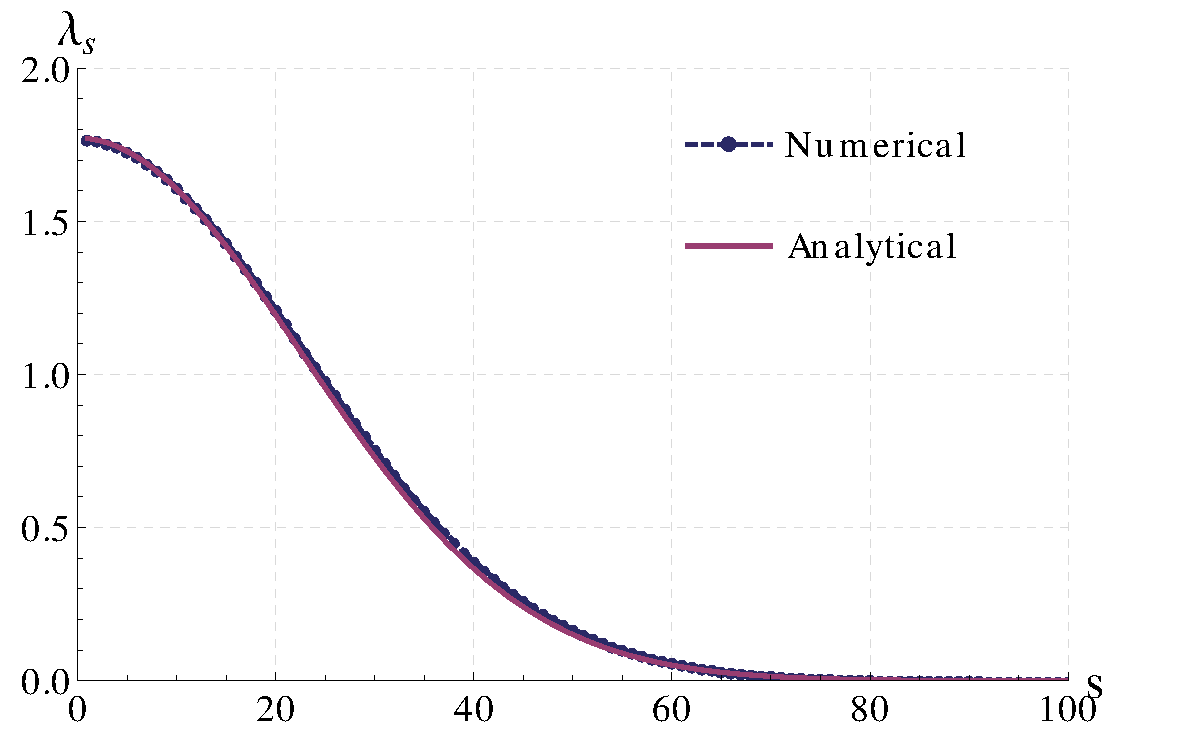
\includegraphics[scale=0.325]{Results/DNA/Eigensystem/T/0.25/lambda_s_L50_m100.pdf}}
\end{tabular}
\caption{Numerical and analytical eigenvalue plots for $\lambda_{s}$ where $\Delta=0.25$.}
\label{fig:dna_eval_s2} 
\begin{tabular}{cc}
\subfloat[$L=5$ $m=25$]{\label{fig:dna_eval_s_5_25}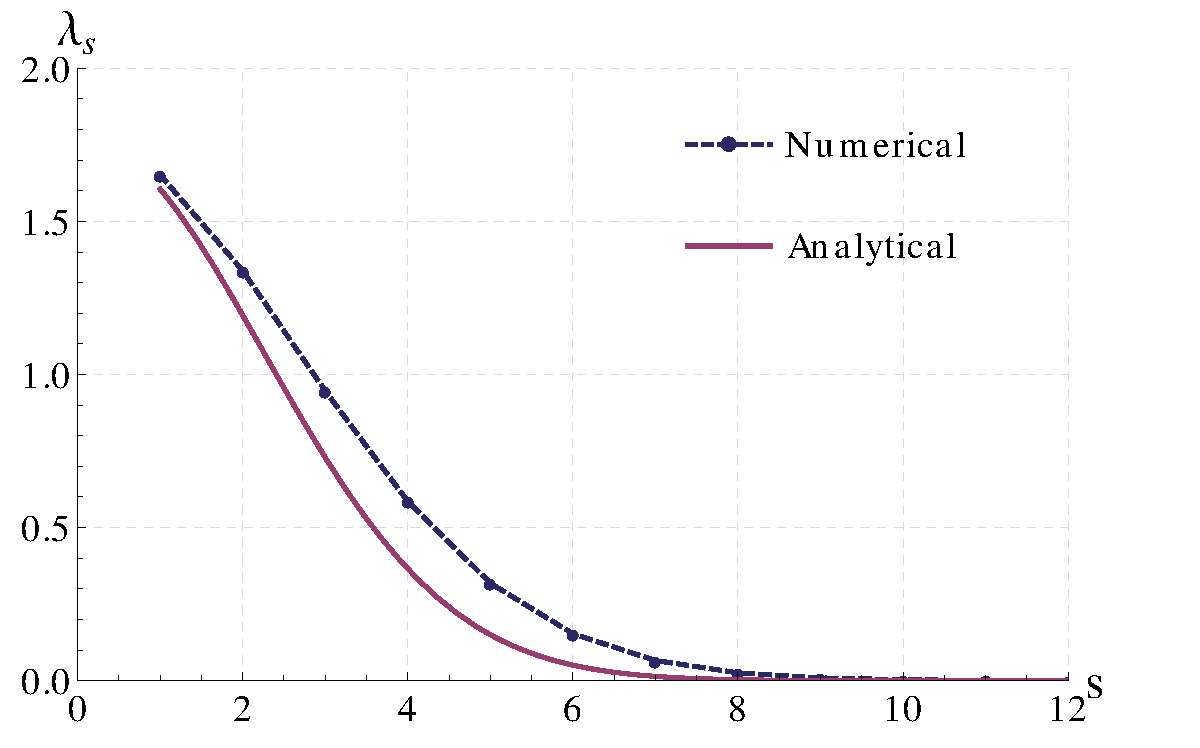
\includegraphics[scale=0.325]{Results/DNA/Eigensystem/T/0.1/lambda_s_L5_m25.pdf}} &
\subfloat[$L=10$ $m=50$]{\label{fig:dna_eval_s_10_50}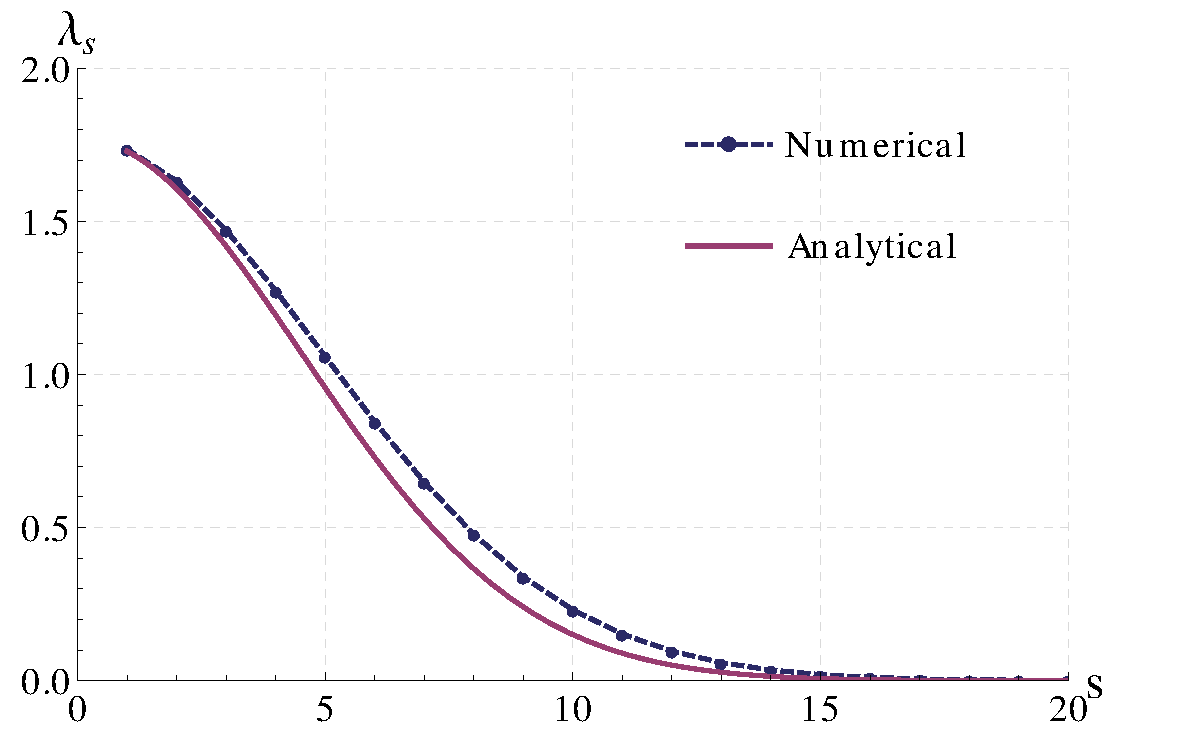
\includegraphics[scale=0.325]{Results/DNA/Eigensystem/T/0.1/lambda_s_L10_m50.pdf}} \\
\subfloat[$L=25$ $m=125$]{\label{fig:dna_eval_s_25_125}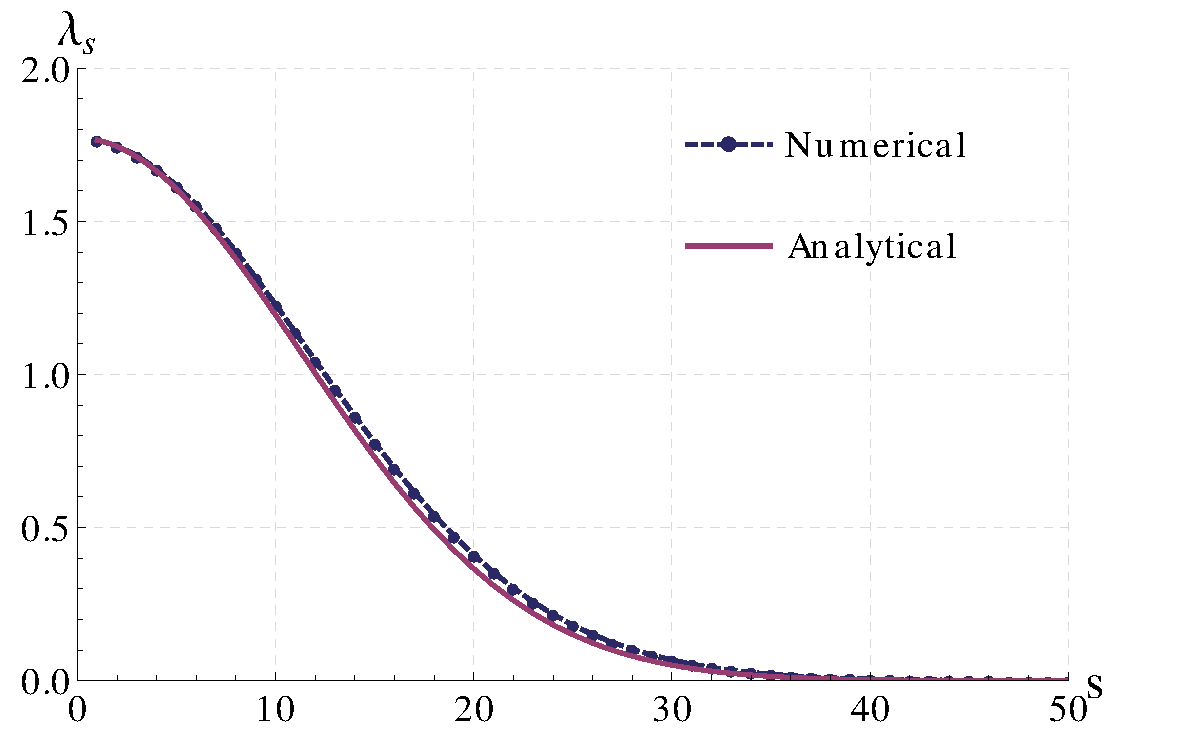
\includegraphics[scale=0.325]{Results/DNA/Eigensystem/T/0.1/lambda_s_L25_m125.pdf}} &
\subfloat[$L=50$ $m=250$]{\label{fig:dna_eval_s_50_250}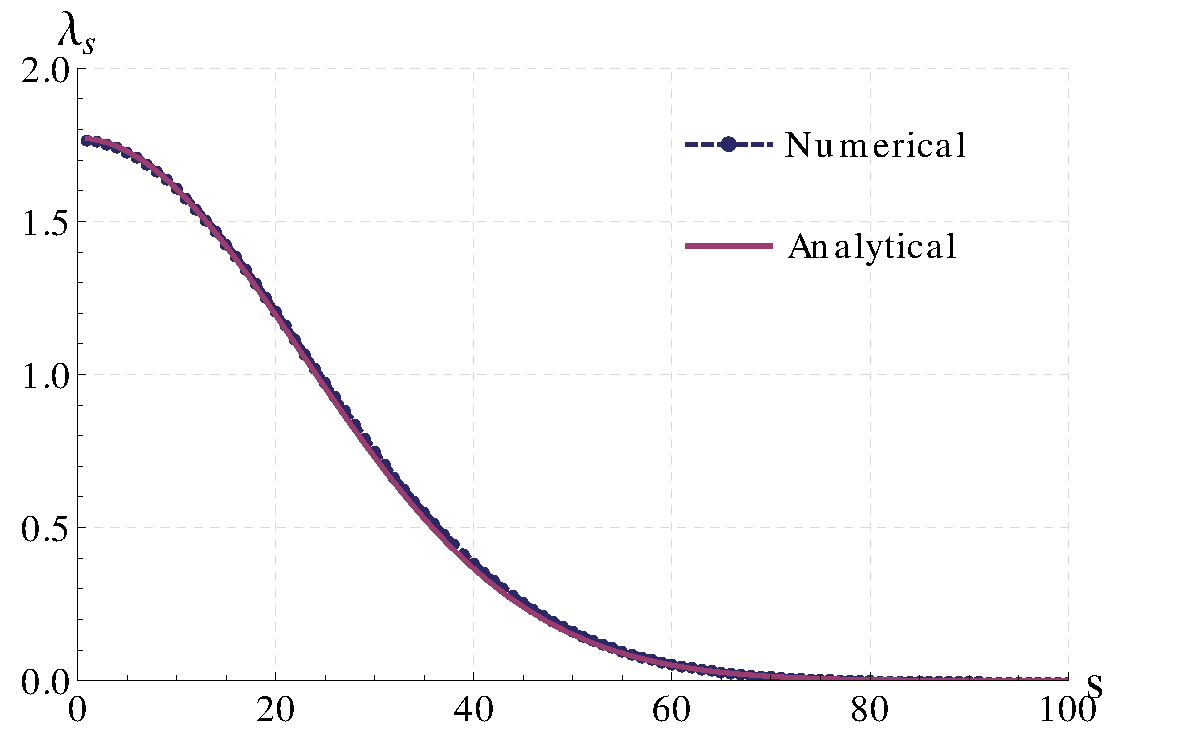
\includegraphics[scale=0.325]{Results/DNA/Eigensystem/T/0.1/lambda_s_L50_m250.pdf}} 
\end{tabular}
\caption{Numerical and analytical eigenvalue plots for $\lambda_{s}$ where $\Delta=0.1$.}
\label{fig:dna_eval_s3} 
\end{figure}

%%% Eigenvalue T00 %%%
\begin{figure}[H]
\centering
\begin{tabular}{cc}
\subfloat[$L=5$ $m=10$]{\label{fig:dna_eval_t00_5_10_delta0.25}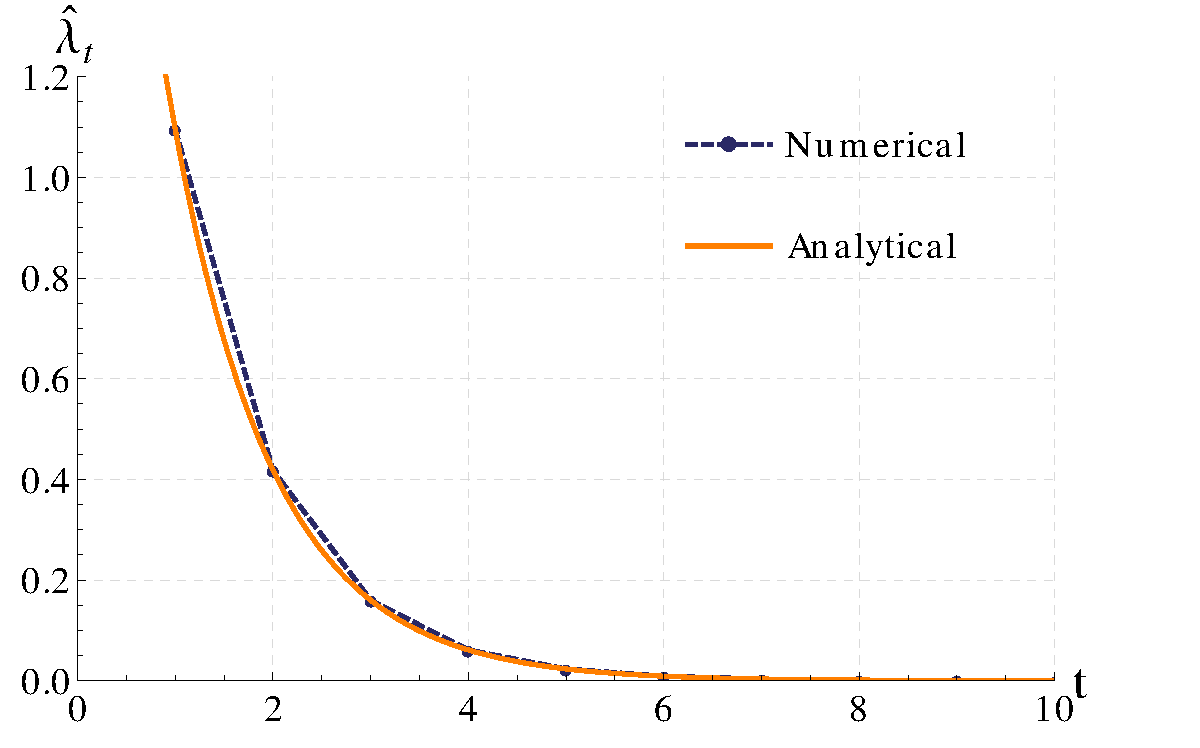
\includegraphics[scale=0.325]{Results/DNA/Eigensystem/T00/0.25/lambda_t_L5_m10.pdf}} &
\subfloat[$L=10$ $m=20$]{\label{fig:dna_eval_t00_10_20_delta0.25}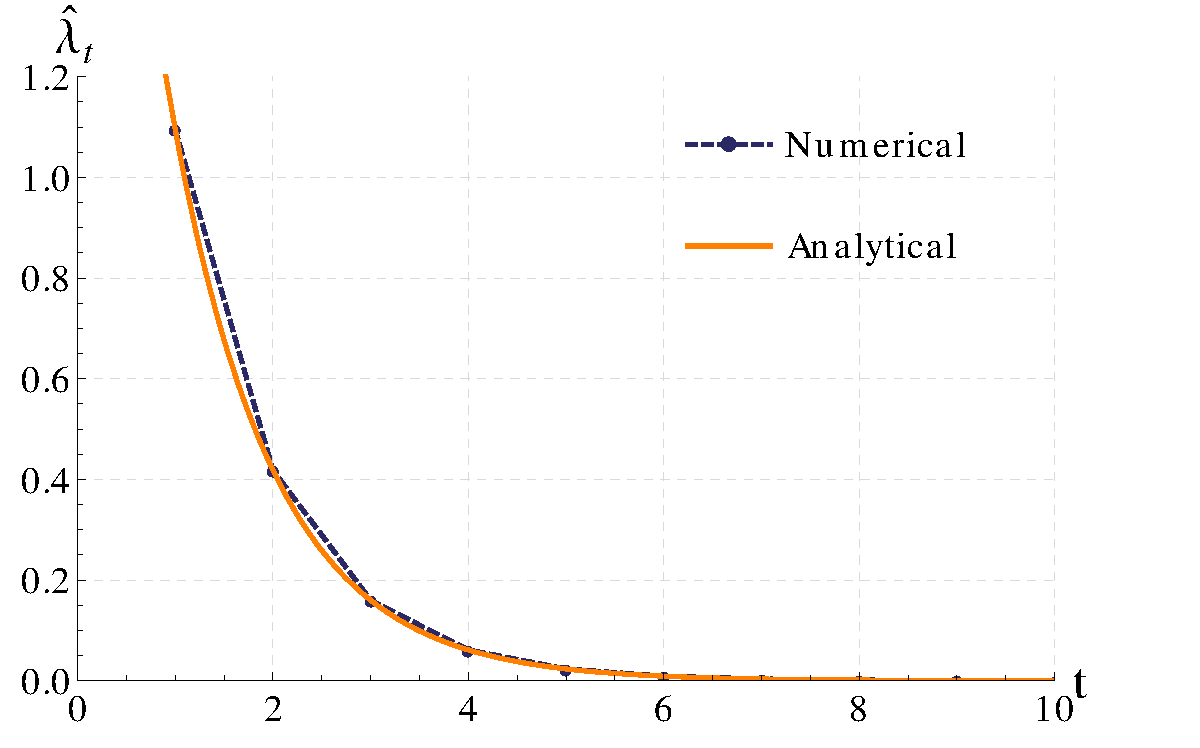
\includegraphics[scale=0.325]{Results/DNA/Eigensystem/T00/0.25/lambda_t_L10_m20.pdf}} \\
\subfloat[$L=25$ $m=50$]{\label{fig:dna_eval_t00_25_50_delta0.25}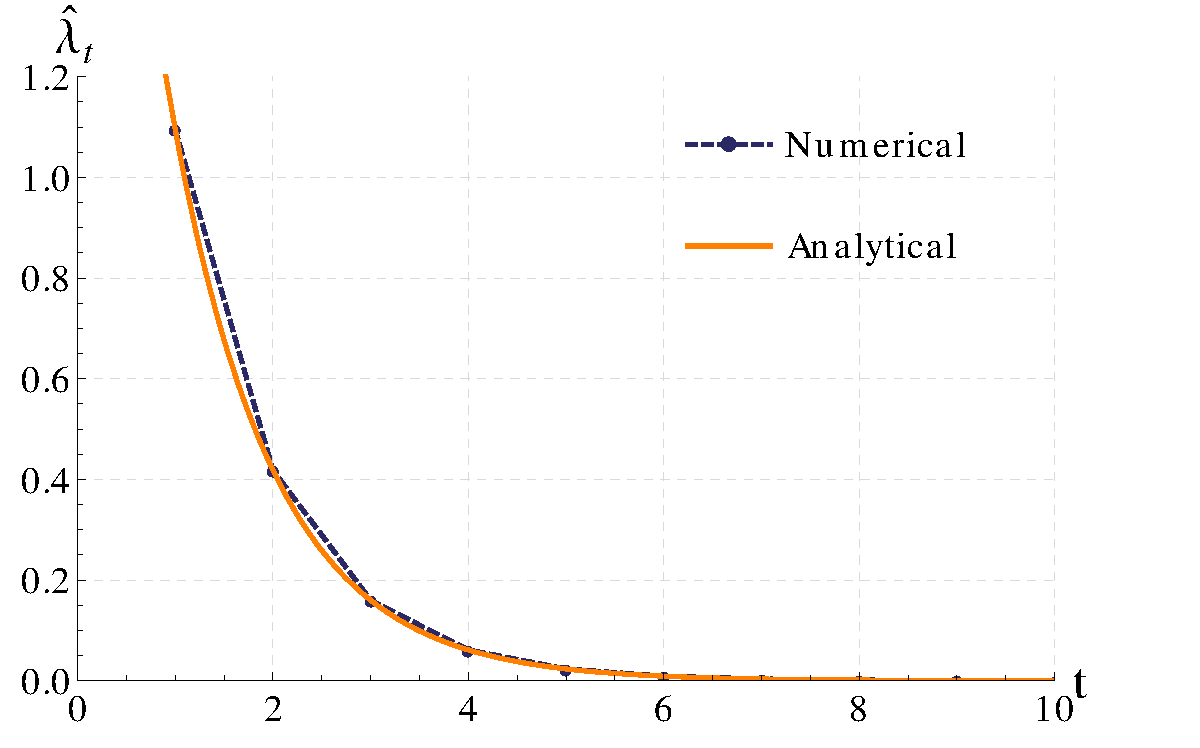
\includegraphics[scale=0.325]{Results/DNA/Eigensystem/T00/0.25/lambda_t_L25_m50.pdf}} &
\subfloat[$L=50$ $m=100$]{\label{fig:dna_eval_t00_50_100_delta0.25}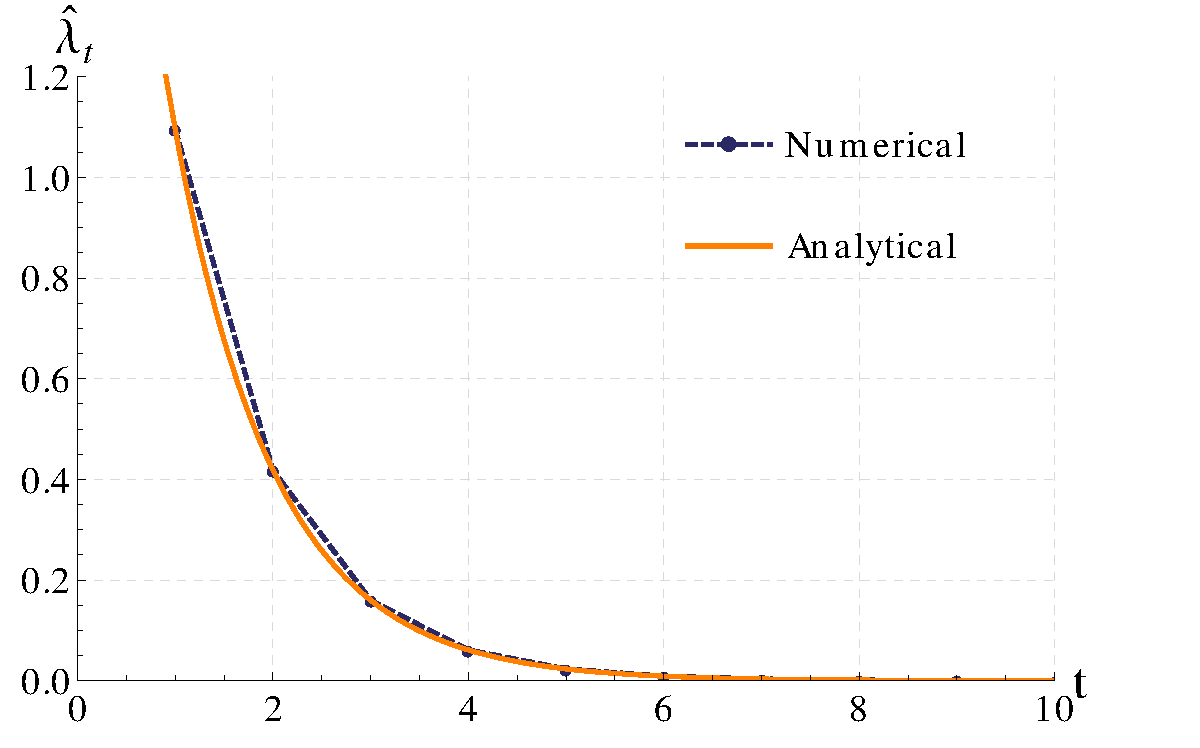
\includegraphics[scale=0.325]{Results/DNA/Eigensystem/T00/0.25/lambda_t_L50_m100.pdf}}
\end{tabular}
\caption{Numerical and analytical eigenvalue plots of $\hat{\lambda}_{t}$ where $\Delta=0.25$.}
\label{fig:dna_eval_t00_delta0.25} 
\begin{tabular}{cc}
\subfloat[$L=5$ $m=5$]{\label{fig:dna_eval_t00_5_5_delta0.5}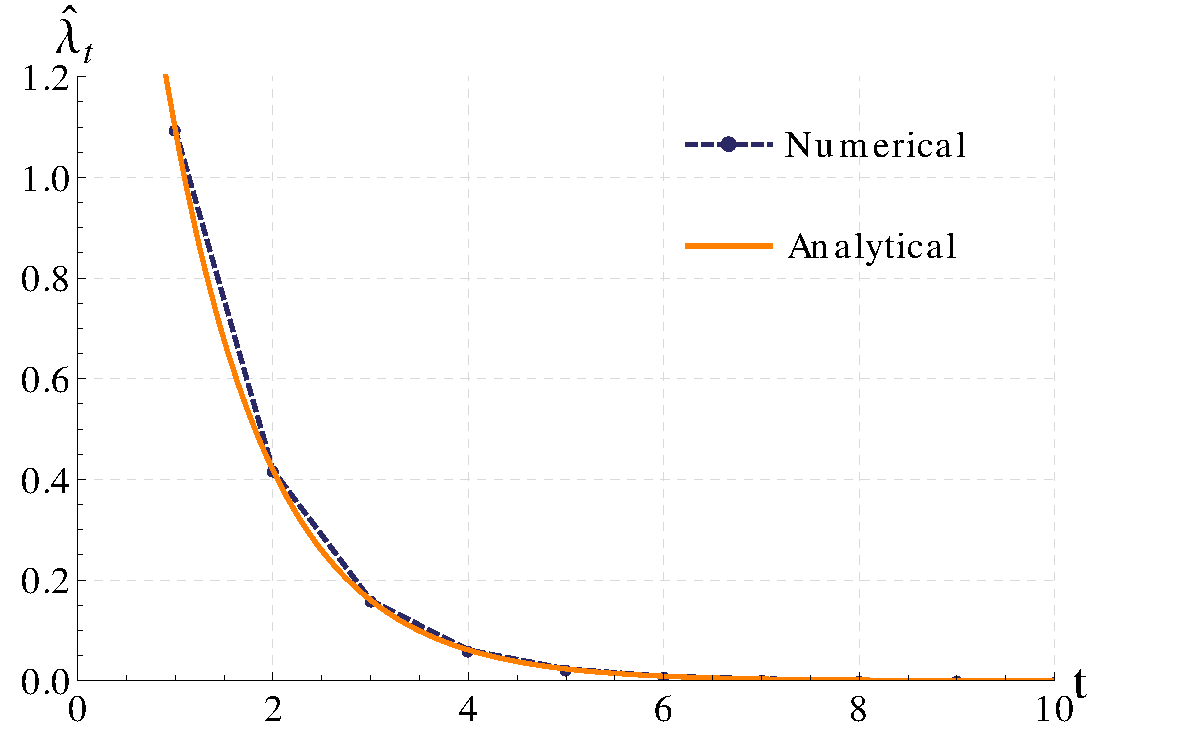
\includegraphics[scale=0.325]{Results/DNA/Eigensystem/T00/0.5/lambda_t_L5_m5.pdf}} &
\subfloat[$L=10$ $m=10$]{\label{fig:dna_eval_t00_10_10_delta0.5}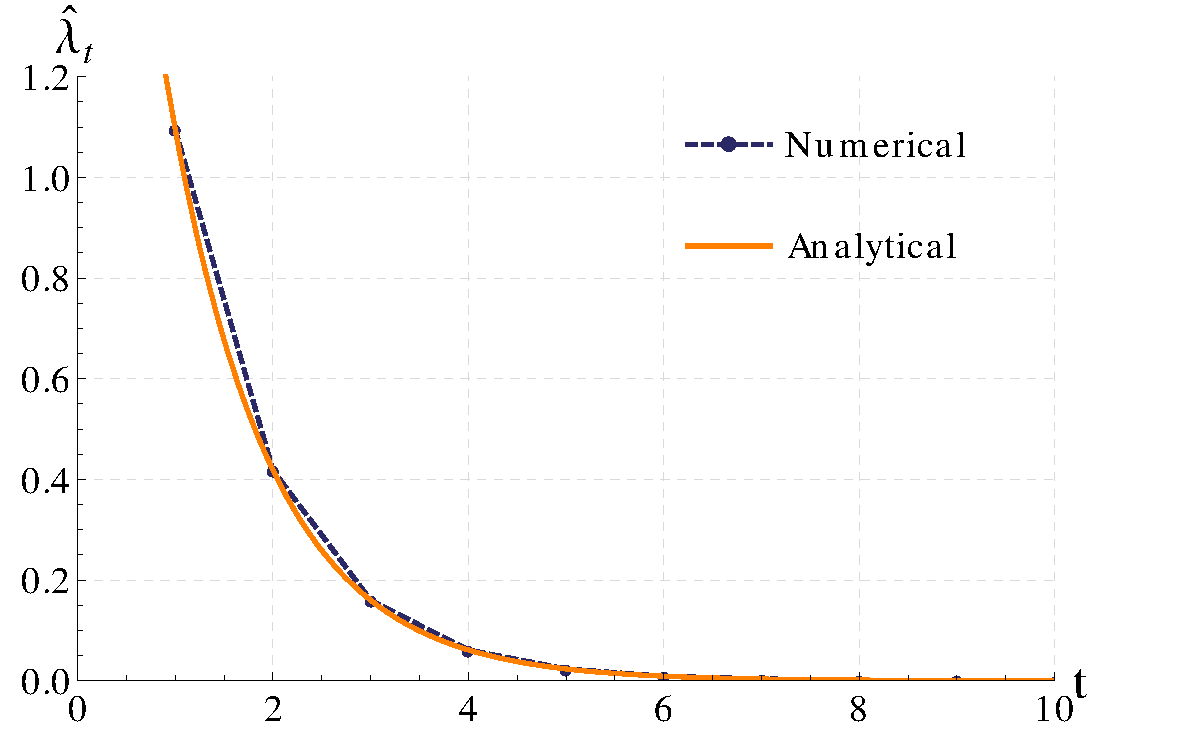
\includegraphics[scale=0.325]{Results/DNA/Eigensystem/T00/0.5/lambda_t_L10_m10.pdf}} \\
\subfloat[$L=25$ $m=25$]{\label{fig:dna_eval_t00_25_25_delta0.5}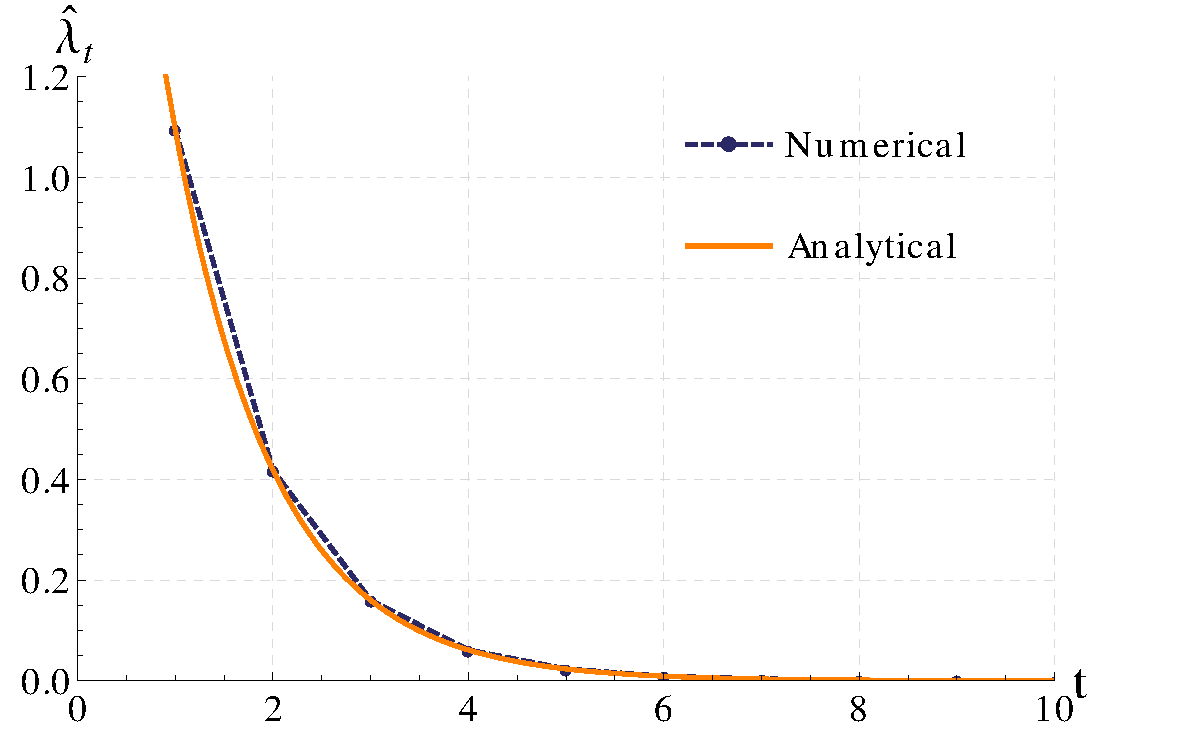
\includegraphics[scale=0.325]{Results/DNA/Eigensystem/T00/0.5/lambda_t_L25_m25.pdf}} &
\subfloat[$L=50$ $m=50$]{\label{fig:dna_eval_t00_50_50_delta0.5}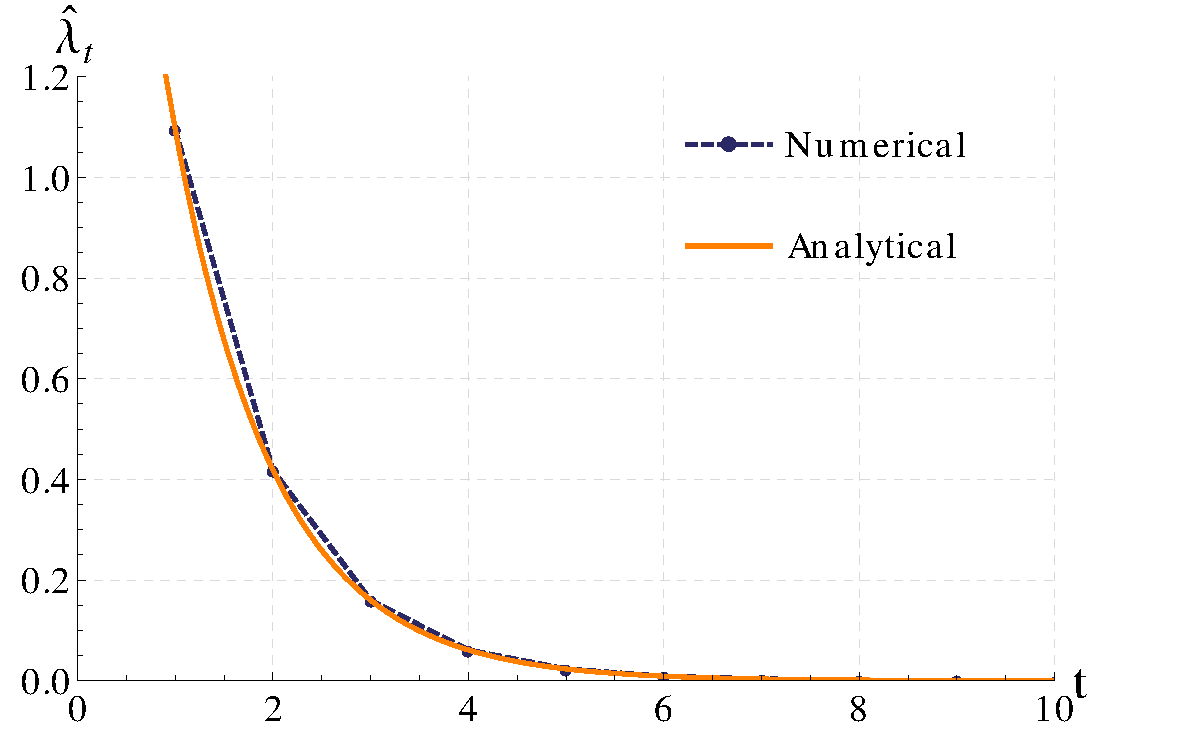
\includegraphics[scale=0.325]{Results/DNA/Eigensystem/T00/0.5/lambda_t_L50_m50.pdf}}
\end{tabular}
\caption{Numerical and analytical eigenvalue plots of $\hat{\lambda}_{t}$ where $\Delta=0.5$.}
\label{fig:dna_eval_t00_delta0.5} 
\end{figure}

%%%% 3D Eigenvalue %%%
%\begin{figure}[H]
%\centering
%\begin{tabular}{cc}
%\subfloat[$t$=1]{\label{fig:dna_eval3D_t00_1_delta0.25}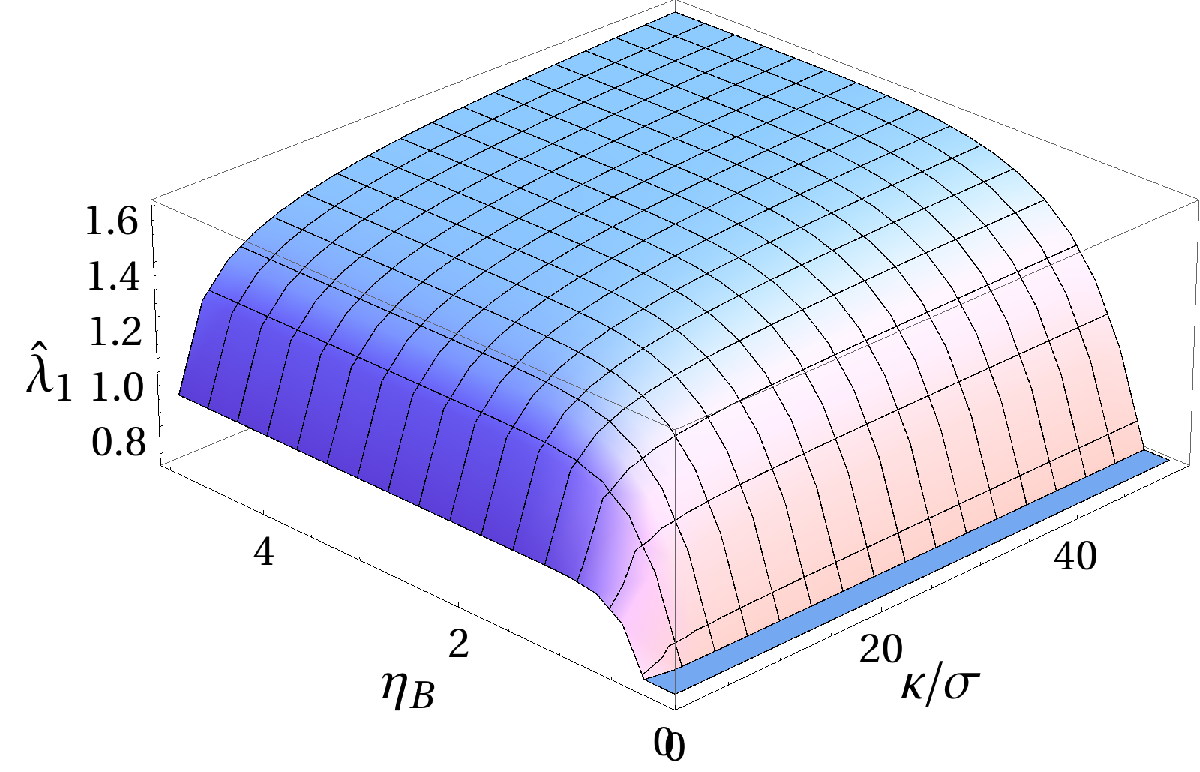
\includegraphics[scale=0.3]{Results/DNA/Eigensystem/%T00/0.25/3D_lambda_t00_t1_L50_m100.pdf}} &
%\hspace{10mm}
%\subfloat[$t$=2]{\label{fig:dna_eval3D_t00_2_delta0.25}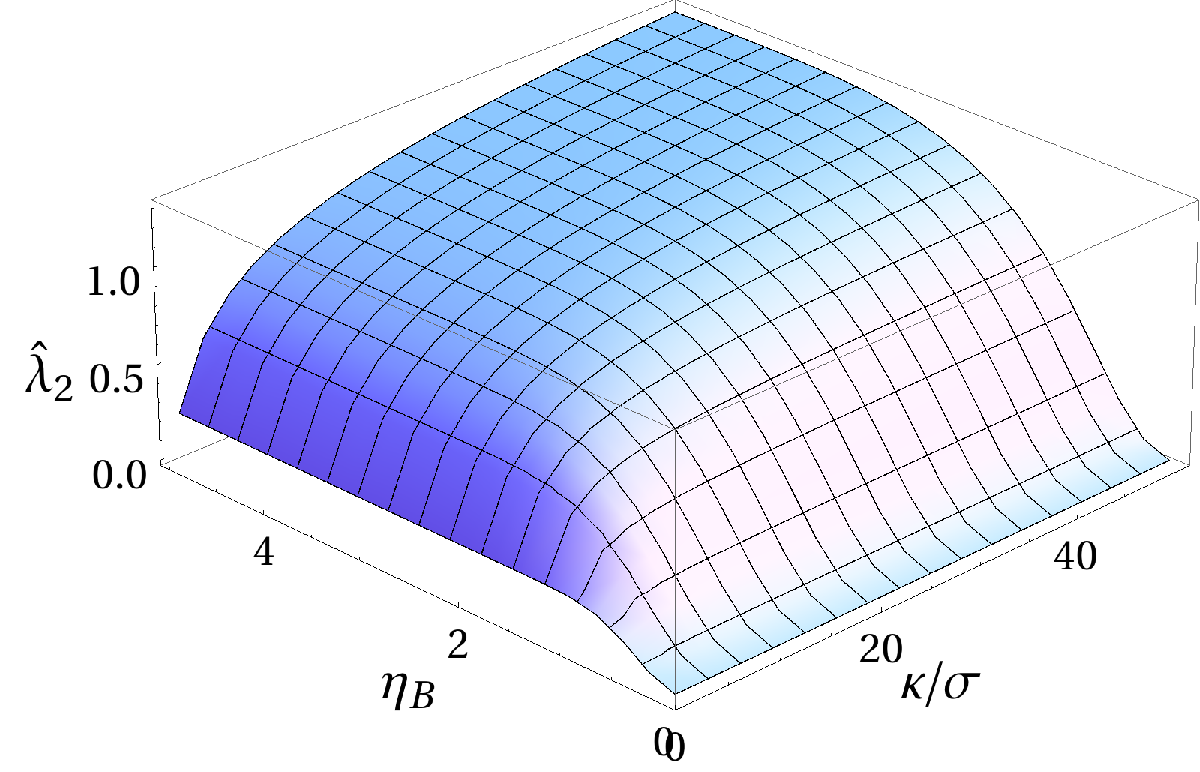
\includegraphics[scale=0.3]{Results/DNA/Eigensystem/%T00/0.25/3D_lambda_t00_t2_L50_m100.pdf}} \\
%\subfloat[$t$=3]{\label{fig:dna_eval3D_t00_3_delta0.25}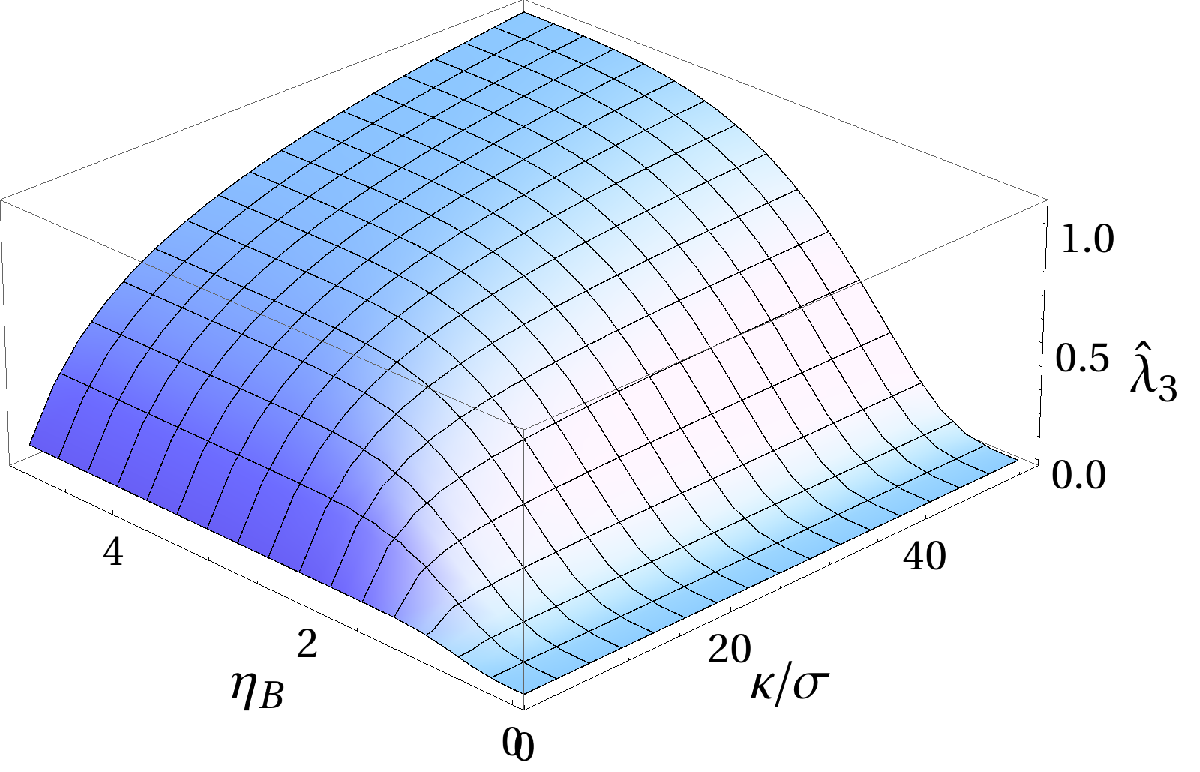
\includegraphics[scale=0.3]{Results/DNA/Eigensystem/T00/0.25/3D_lambda_t00_t3_L50_m100.pdf}} &
%\hspace{10mm}
%\subfloat[$t$=4]{\label{fig:dna_eval3D_t00_4_delta0.25}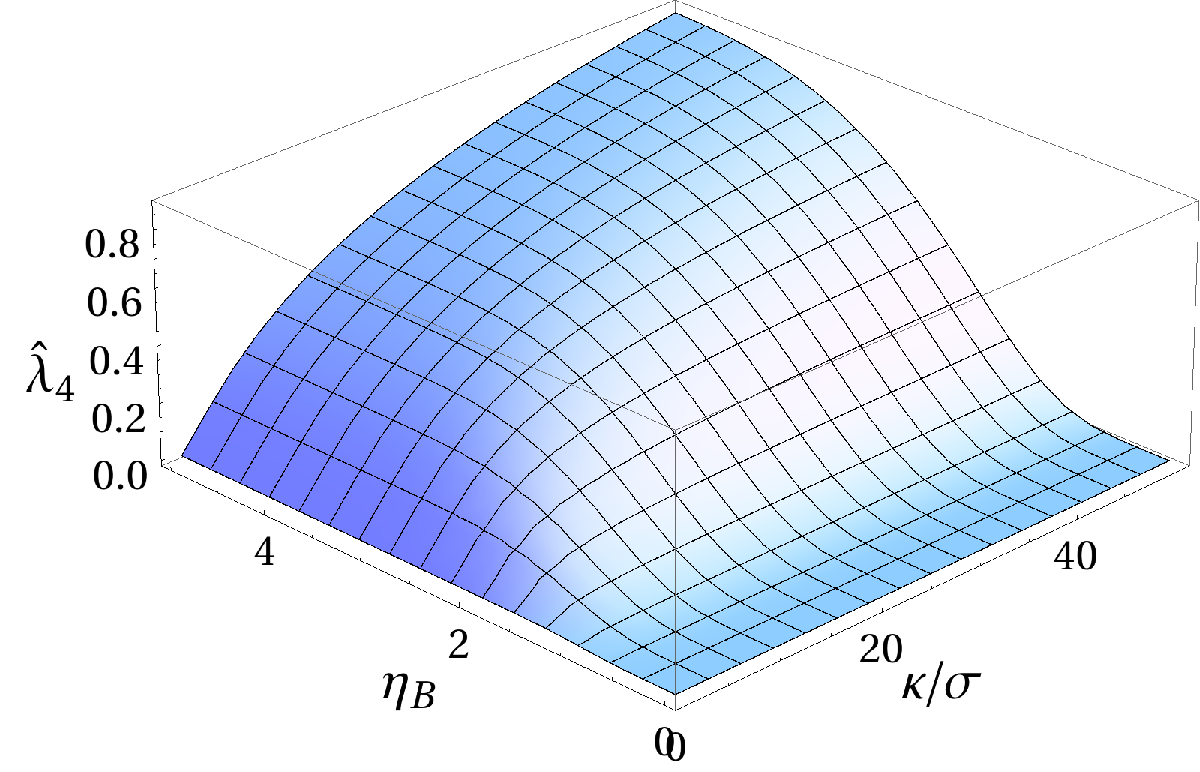
\includegraphics[scale=0.3]{Results/DNA/Eigensystem/T00/0.25/3D_lambda_t00_t4_L50_m100.pdf}}
%\end{tabular}
%\caption{3D eigenvalue plots demonstrating how $\hat{\lambda}_t$ varies against $\kappa/\sigma$ and $\eta_{B}$. These plots have $\Delta=0.25$ ($L$=50 and $m$=100).}
%\label{fig:dna_eval3D_t00_delta0.25} 
%\begin{tabular}{cc}
%\subfloat[$t$=1]{\label{fig:dna_eval3D_t11_1_delta0.25}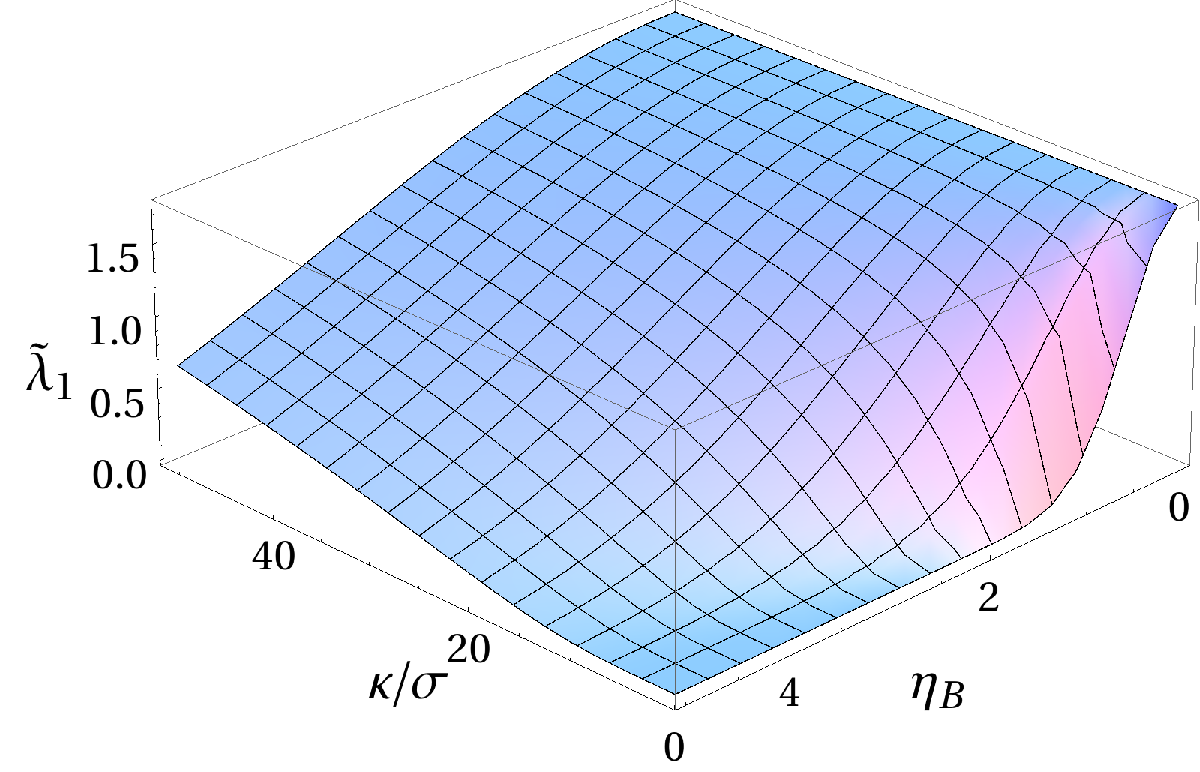
\includegraphics[scale=0.3]{Results/DNA/Eigensystem/T11/0.25/3D_lambda_t11_t1_L50_m100.pdf}} &
%\hspace{10mm}
%\subfloat[$t$=2]{\label{fig:dna_eval3D_t11_2_delta0.25}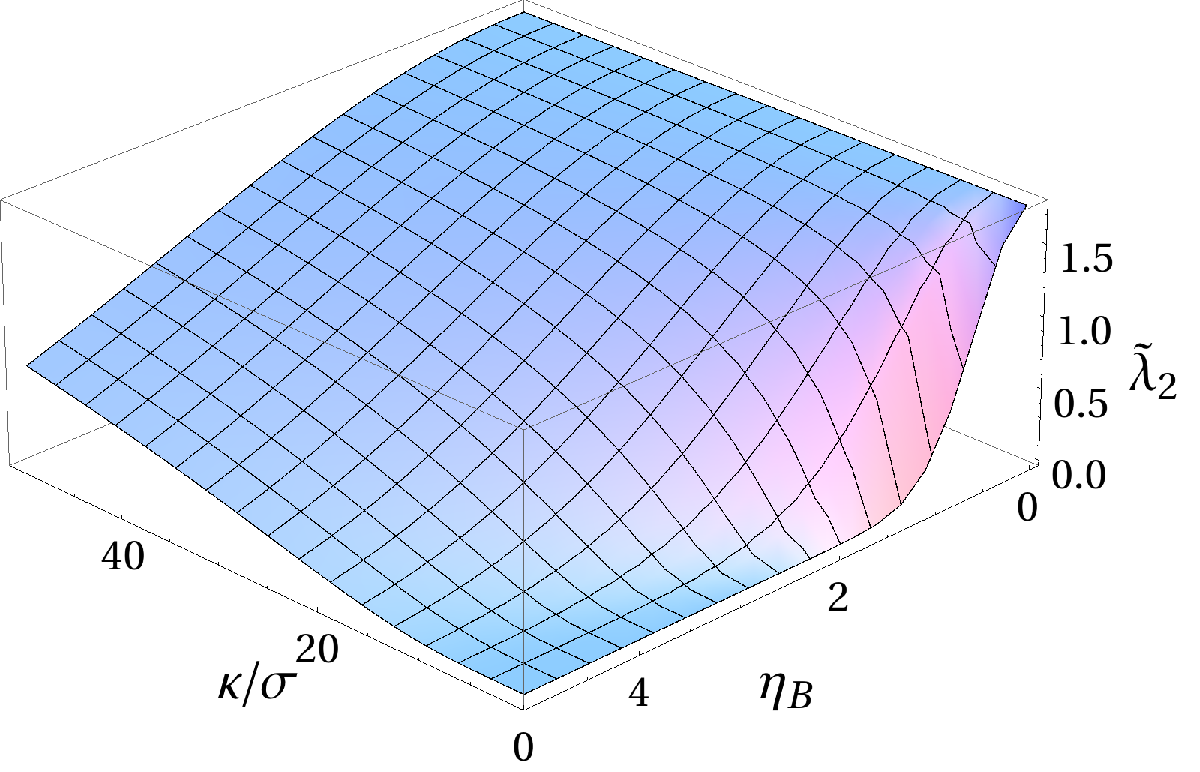
\includegraphics[scale=0.3]{Results/DNA/Eigensystem/T11/0.25/3D_lambda_t11_t2_L50_m100.pdf}} \\
%\subfloat[$t$=3]{\label{fig:dna_eval3D_t11_3_delta0.25}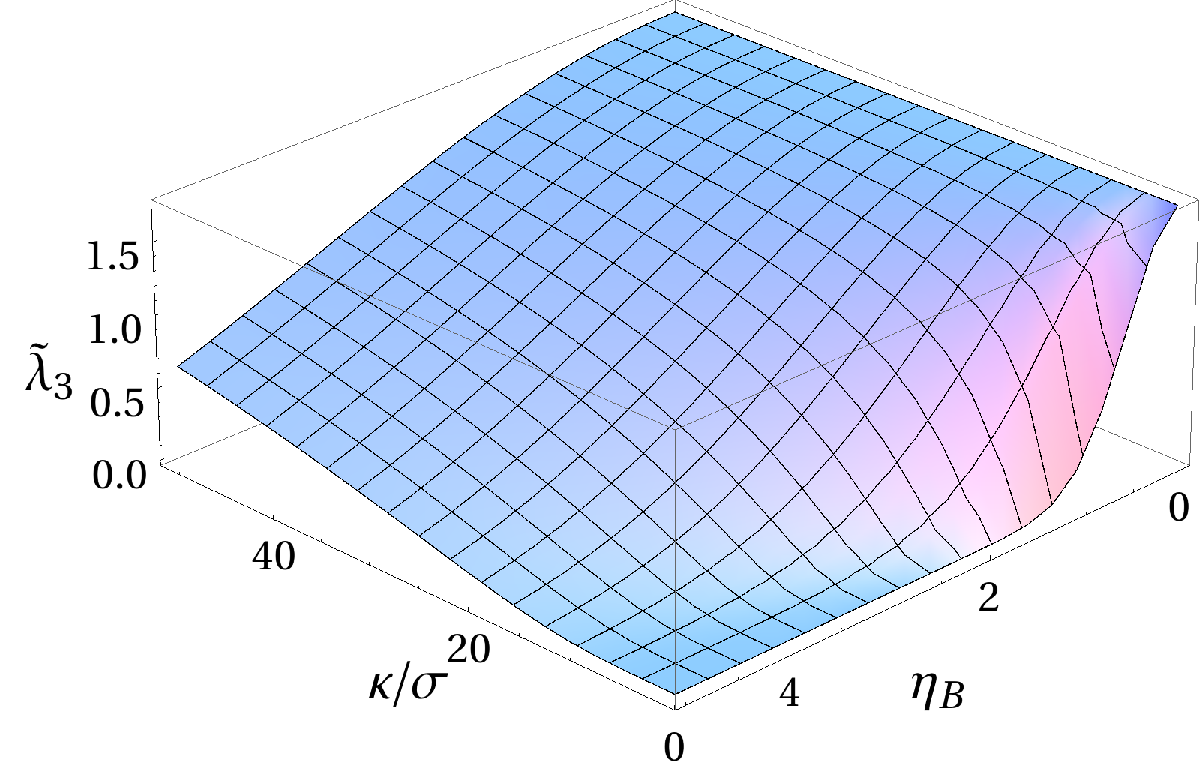
\includegraphics[scale=0.3]{Results/DNA/Eigensystem/T11/0.25/3D_lambda_t11_t3_L50_m100.pdf}} &
%\hspace{10mm}
%\subfloat[$t$=4]{\label{fig:dna_eval3D_t11_4_delta0.25}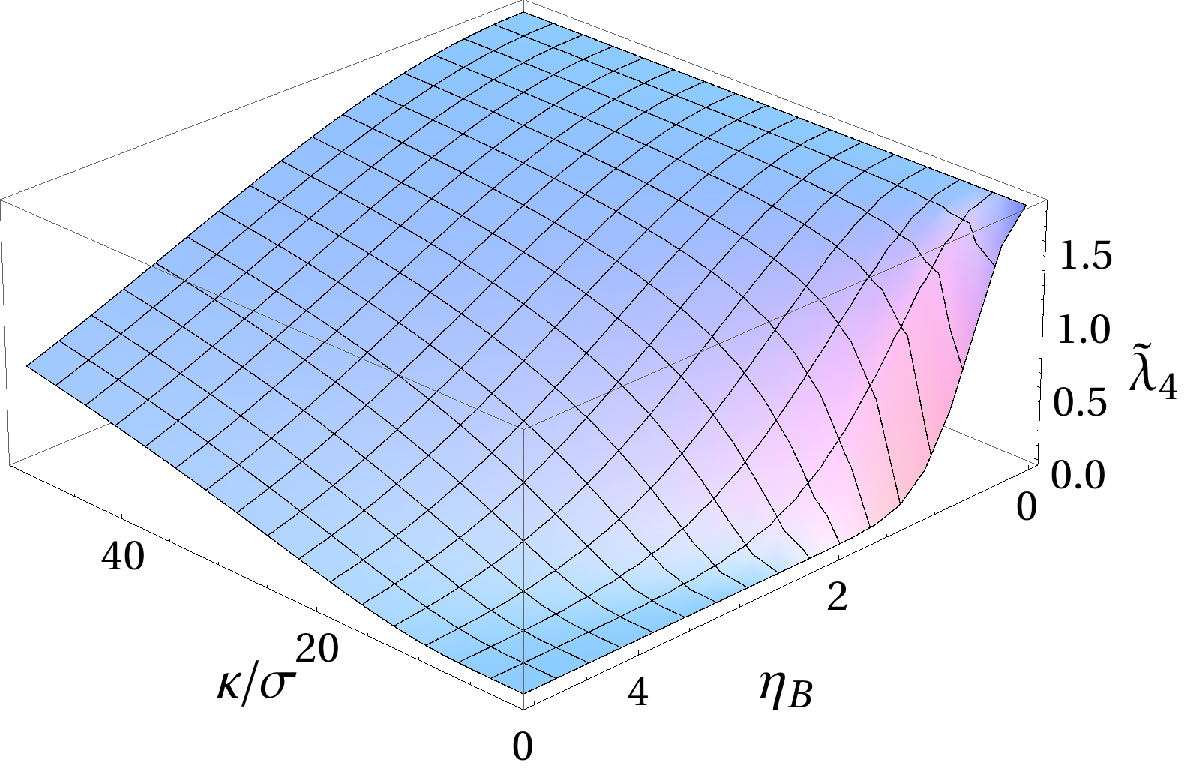
\includegraphics[scale=0.3]{Results/DNA/Eigensystem/T11/0.25/3D_lambda_t11_t4_L50_m100.pdf}}
%\end{tabular}
%\caption{3D eigenvalue plots demonstrating how $\hat{\lambda}_t$ varies against $\kappa/\sigma$ and $\eta_{B}$. These plots have $\Delta=0.25$ ($L$=50 and $m$=100).}
%\label{fig:dna_eval3D_t11_delta0.25} 
%\end{figure}

%%% Numerical vs Analytical calculations of Eigenfunctions T00 %%%
\begin{figure}[H]
\centering
\begin{tabular}{cc}
\subfloat[$t$=0]{\label{fig:nVa_dna_efun_t00_0_delta0.5}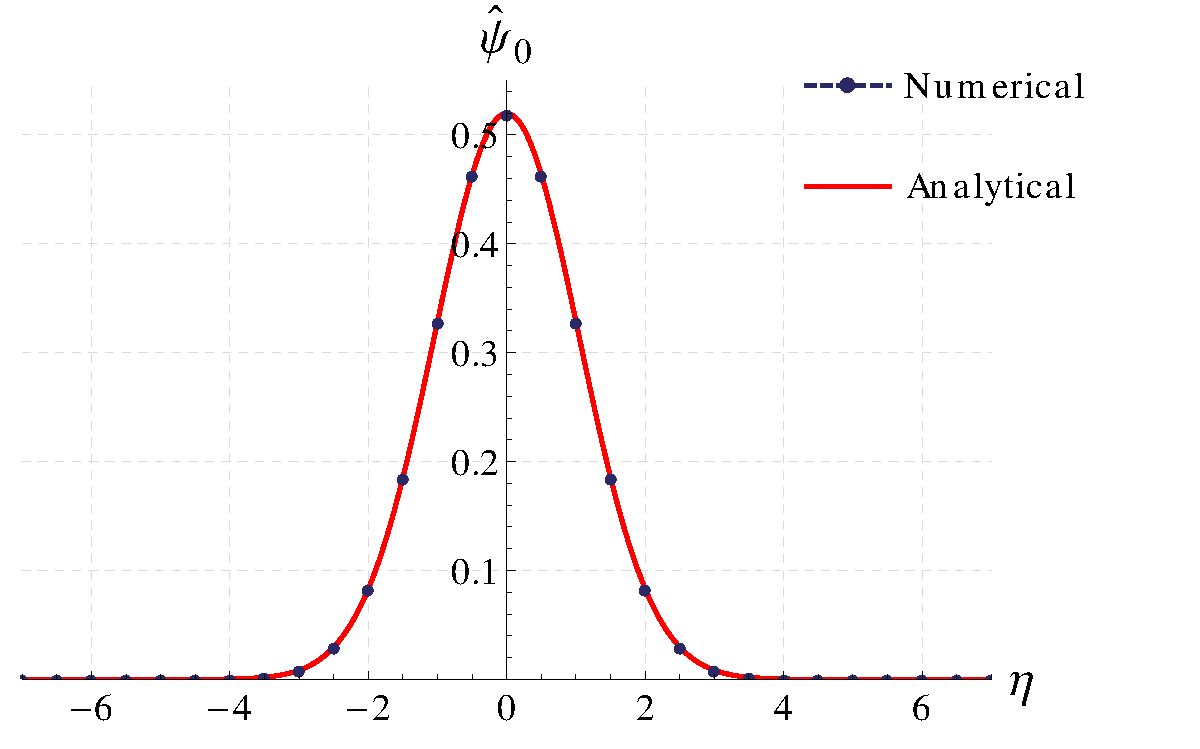
\includegraphics[scale=0.325]{Results/DNA/Eigensystem/T00/0.5/nVa_psi_t00_t0_L50_m50_k10_etab25.pdf}} &
\subfloat[$t$=1]{\label{fig:nVa_dna_efun_t00_1_delta0.5}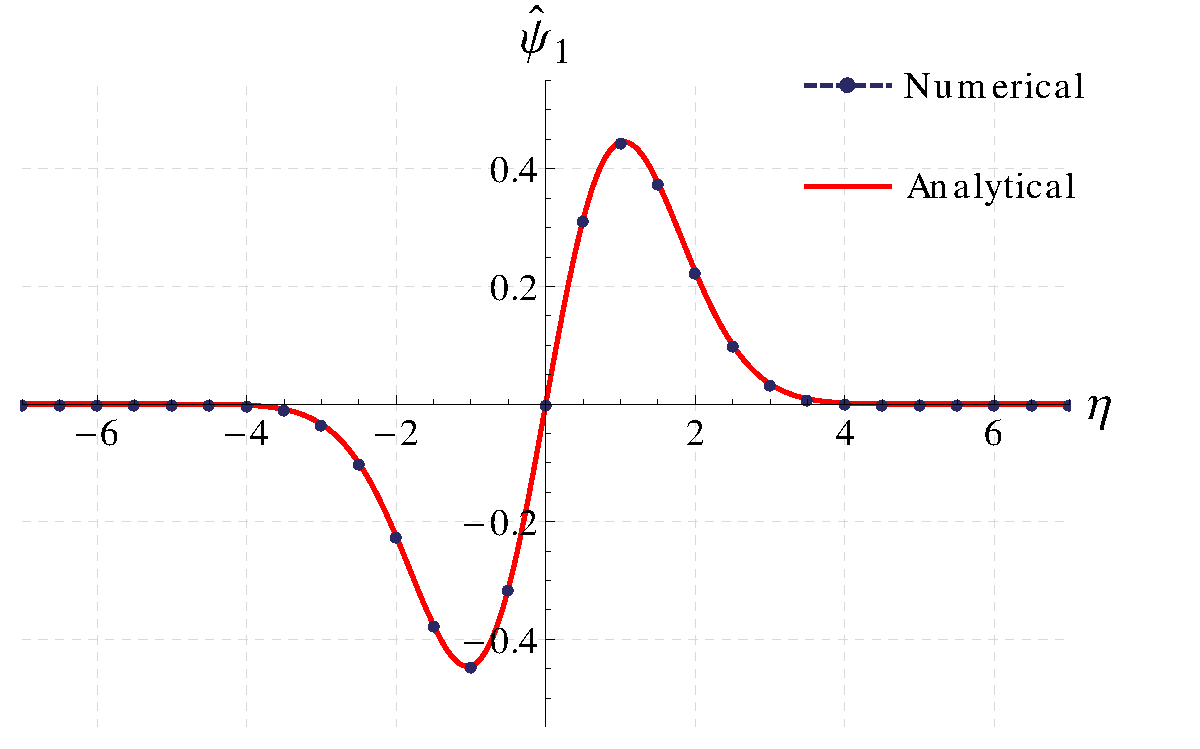
\includegraphics[scale=0.325]{Results/DNA/Eigensystem/T00/0.5/nVa_psi_t00_t1_L50_m50_k10_etab25.pdf}} \\
\subfloat[$t$=2]{\label{fig:nVa_dna_efun_t00_2_delta0.5}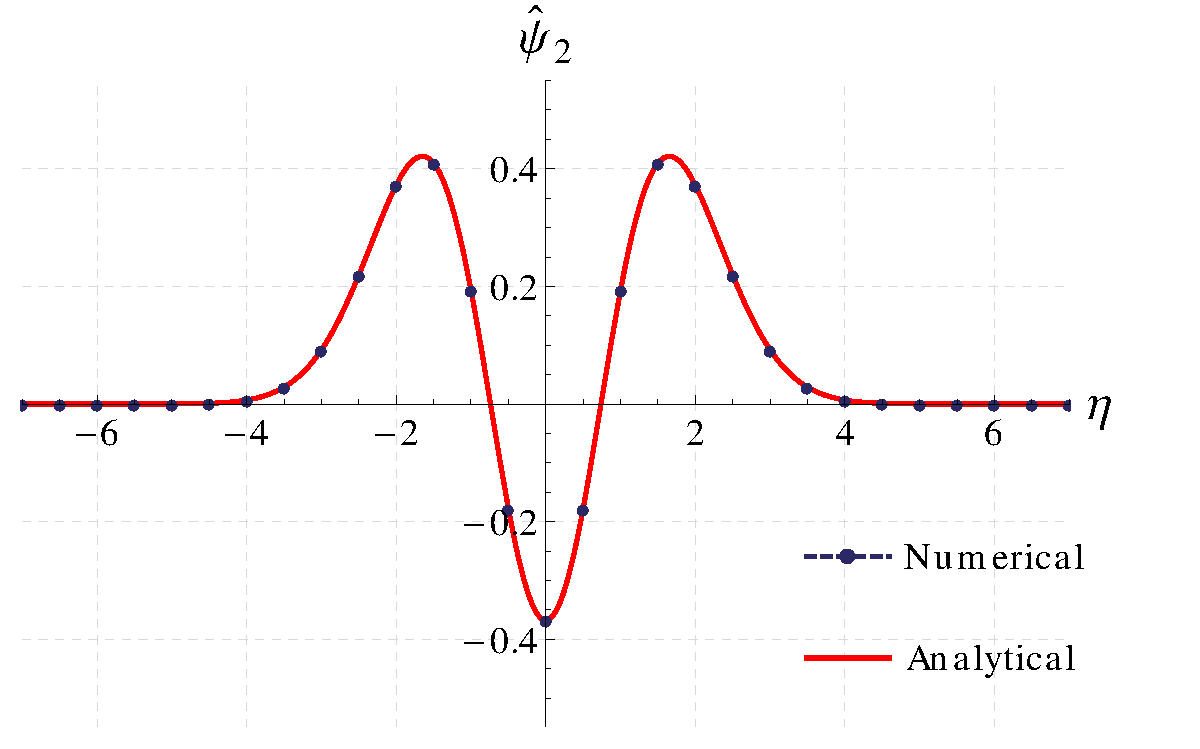
\includegraphics[scale=0.325]{Results/DNA/Eigensystem/T00/0.5/nVa_psi_t00_t2_L50_m50_k10_etab25.pdf}} &
\subfloat[$t$=3]{\label{fig:nVa_dna_efun_t00_3_delta0.5}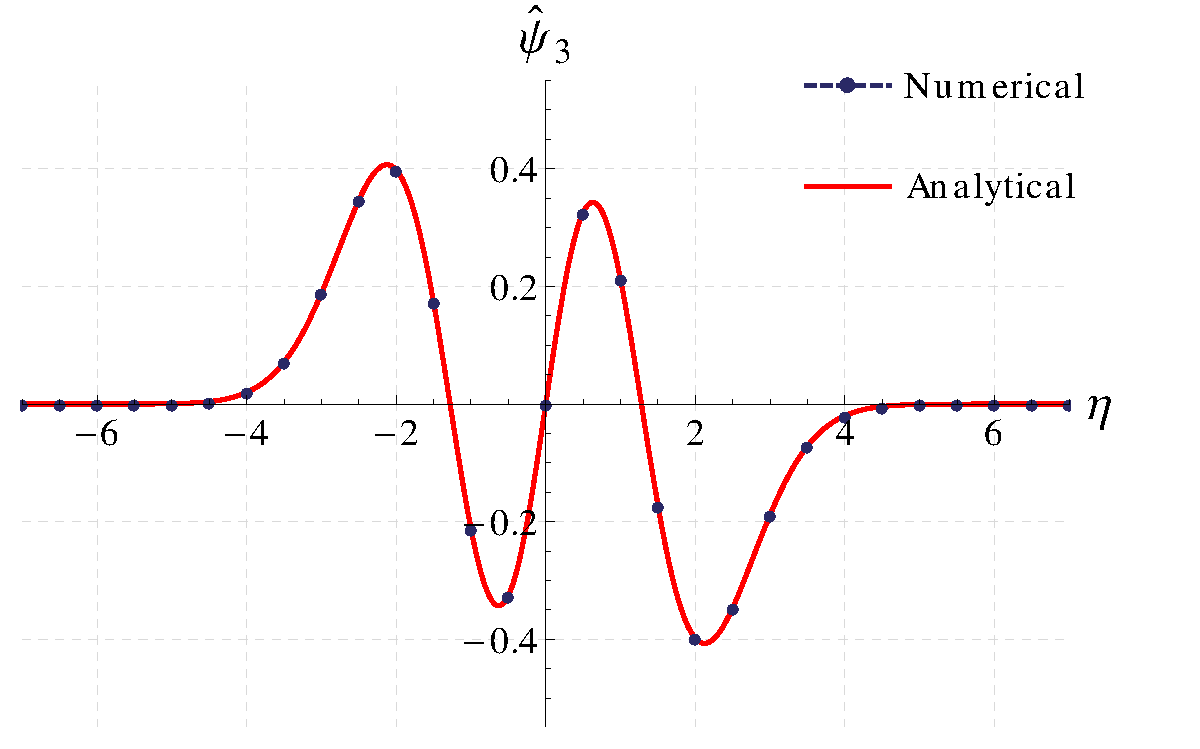
\includegraphics[scale=0.325]{Results/DNA/Eigensystem/T00/0.5/nVa_psi_t00_t3_L50_m50_k10_etab25.pdf}}
\end{tabular}
\caption{Eigenfunction plots of $\hat{\psi}_{t}$ with $\Delta=0.5$ ($L$=50 and $m$=50).}
\label{fig:nVa_dna_psi_t00_delta0.5} 
\begin{tabular}{cc}
\subfloat[$t$=0]{\label{fig:nVa_dna_efun_t00_0_delta0.25}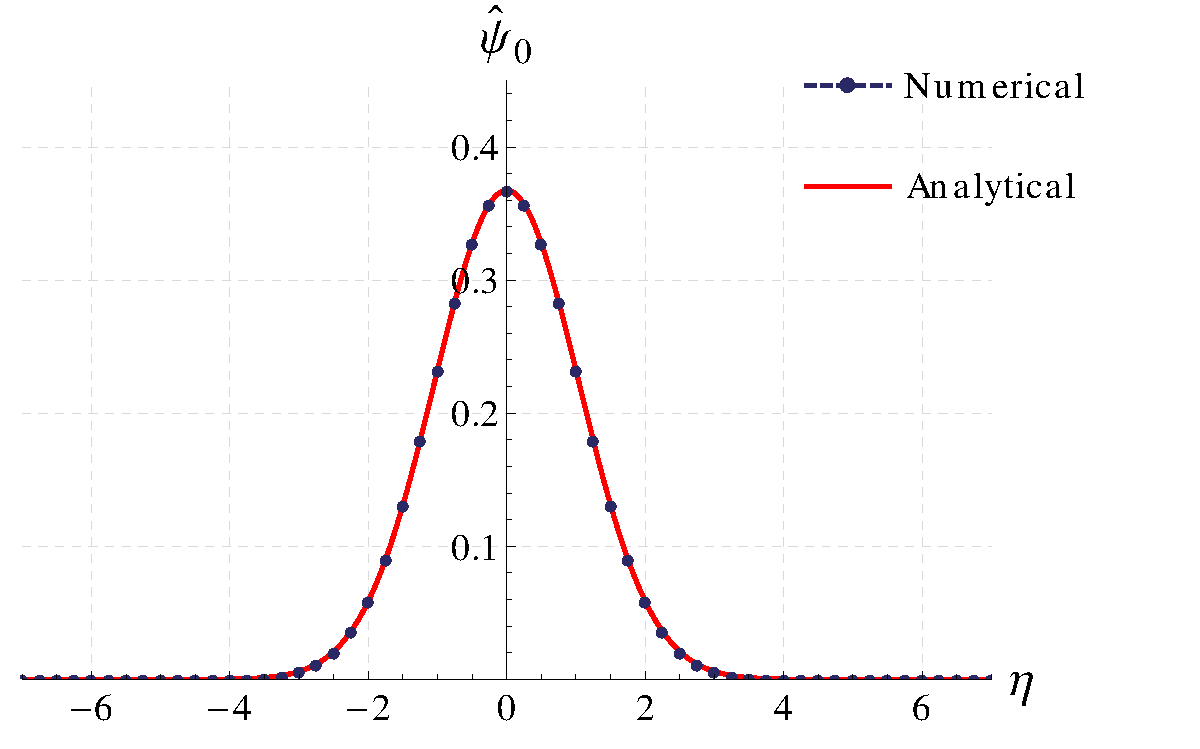
\includegraphics[scale=0.325]{Results/DNA/Eigensystem/T00/0.25/nVa_psi_t00_t0_L50_m100_k10_etab25.pdf}} &
\subfloat[$t$=1]{\label{fig:nVa_dna_efun_t00_1_delta0.25}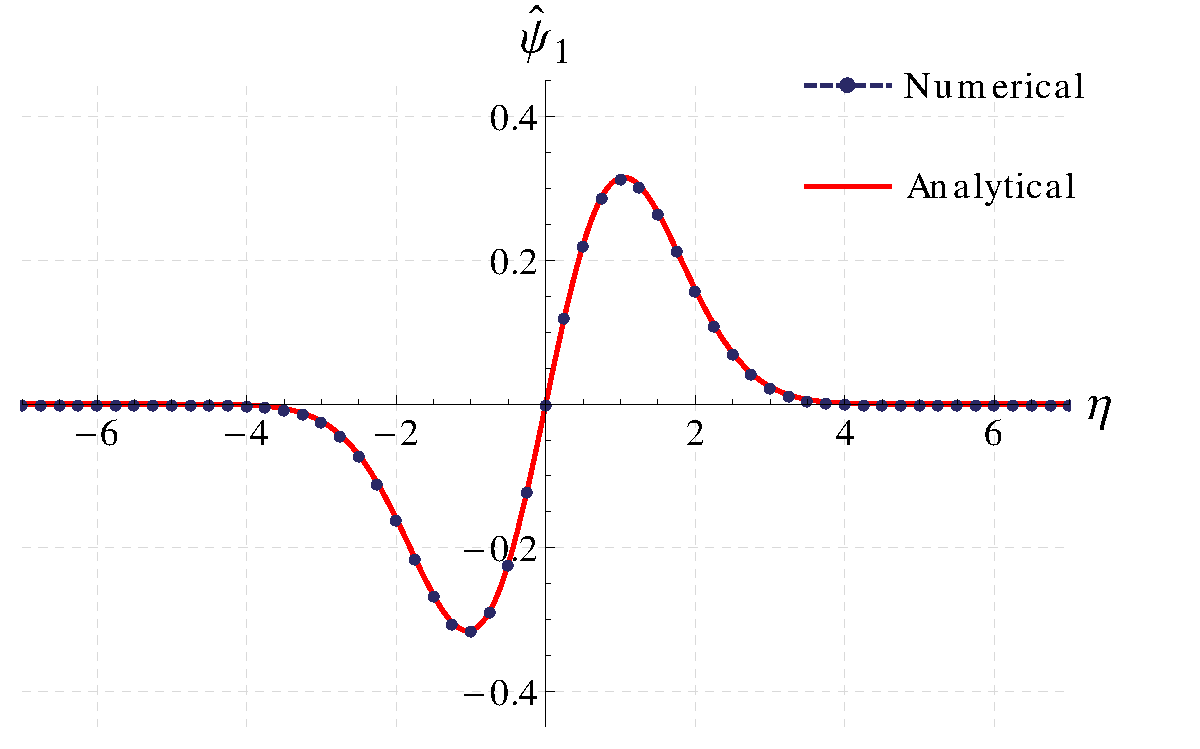
\includegraphics[scale=0.325]{Results/DNA/Eigensystem/T00/0.25/nVa_psi_t00_t1_L50_m100_k10_etab25.pdf}} \\
\subfloat[$t$=2]{\label{fig:nVa_dna_efun_t00_2_delta0.25}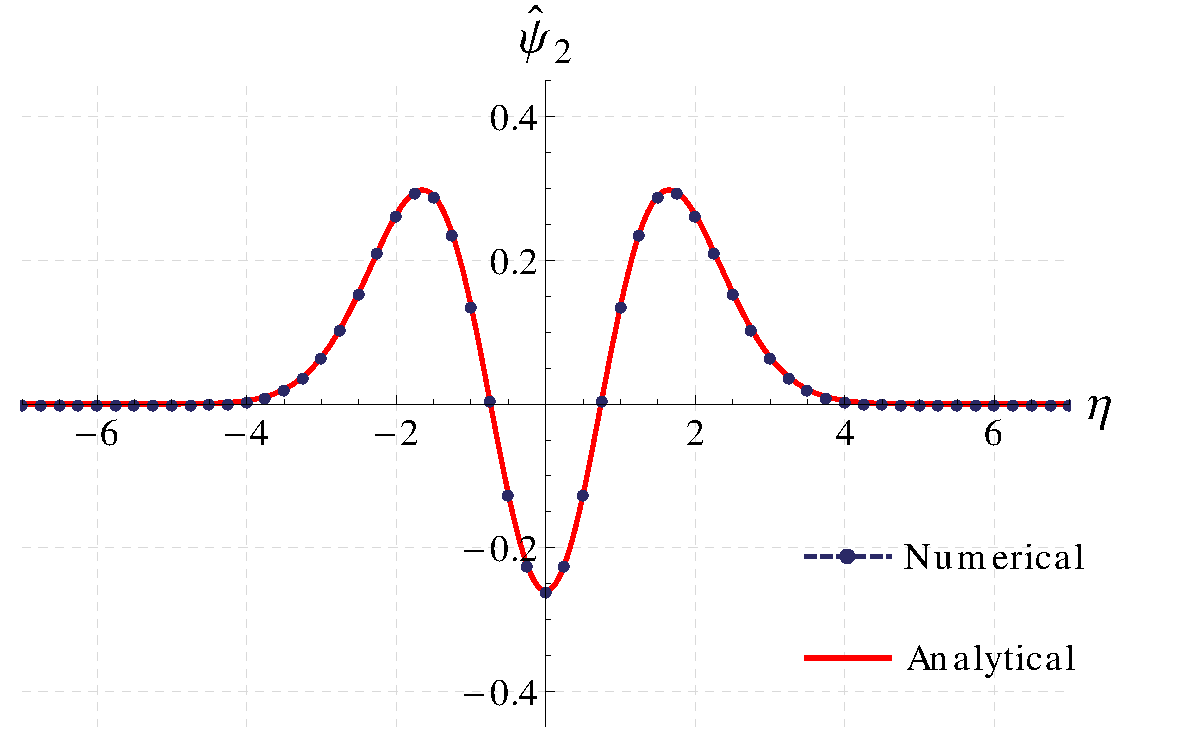
\includegraphics[scale=0.325]{Results/DNA/Eigensystem/T00/0.25/nVa_psi_t00_t2_L50_m100_k10_etab25.pdf}} &
\subfloat[$t$=3]{\label{fig:nVa_dna_efun_t00_3_delta0.25}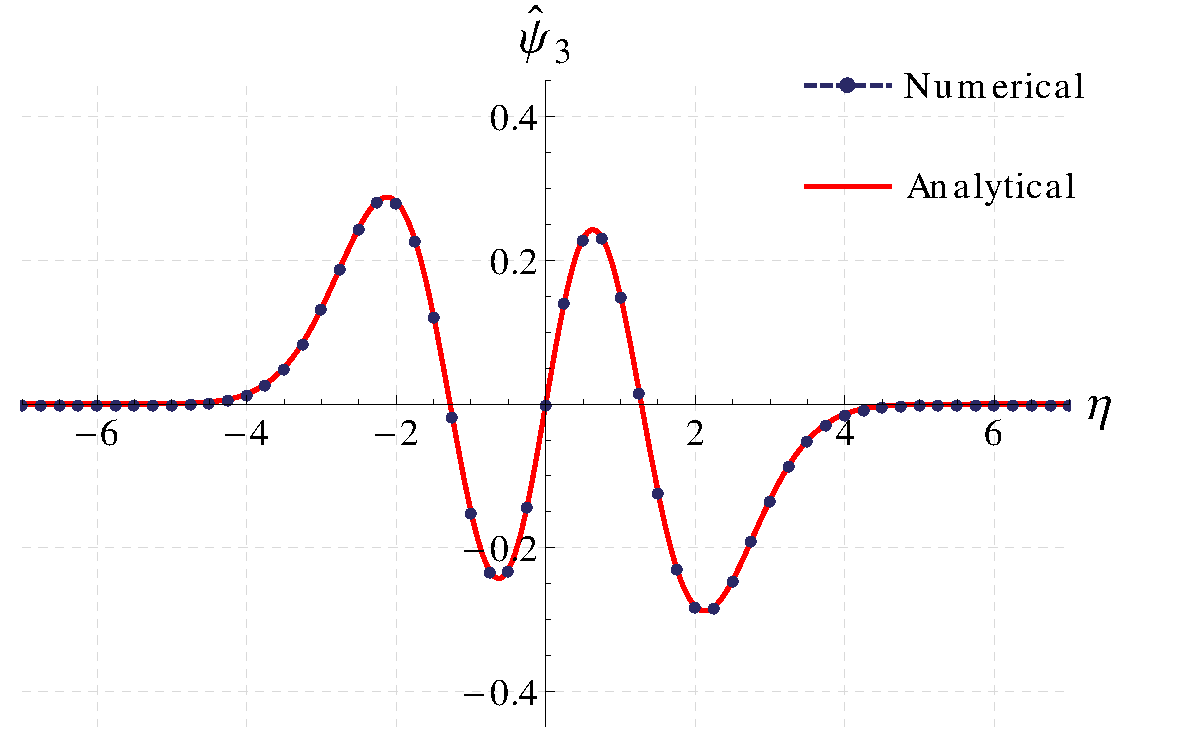
\includegraphics[scale=0.325]{Results/DNA/Eigensystem/T00/0.25/nVa_psi_t00_t3_L50_m100_k10_etab25.pdf}}
\end{tabular}
\caption{Eigenfunction plots of $\hat{\psi}_{t}$ with $\Delta=0.25$ ($L$=50 and $m$=100).}
\label{fig:nVa_dna_psi_t00_delta0.25} 
\end{figure}

%%% Numerical Calculations of Eigenfunctions T00 %%%
\begin{figure}[H]
\centering
\begin{tabular}{cc}
\subfloat[$t$=0]{\label{fig:dna_efun_t00_0_delta0.25}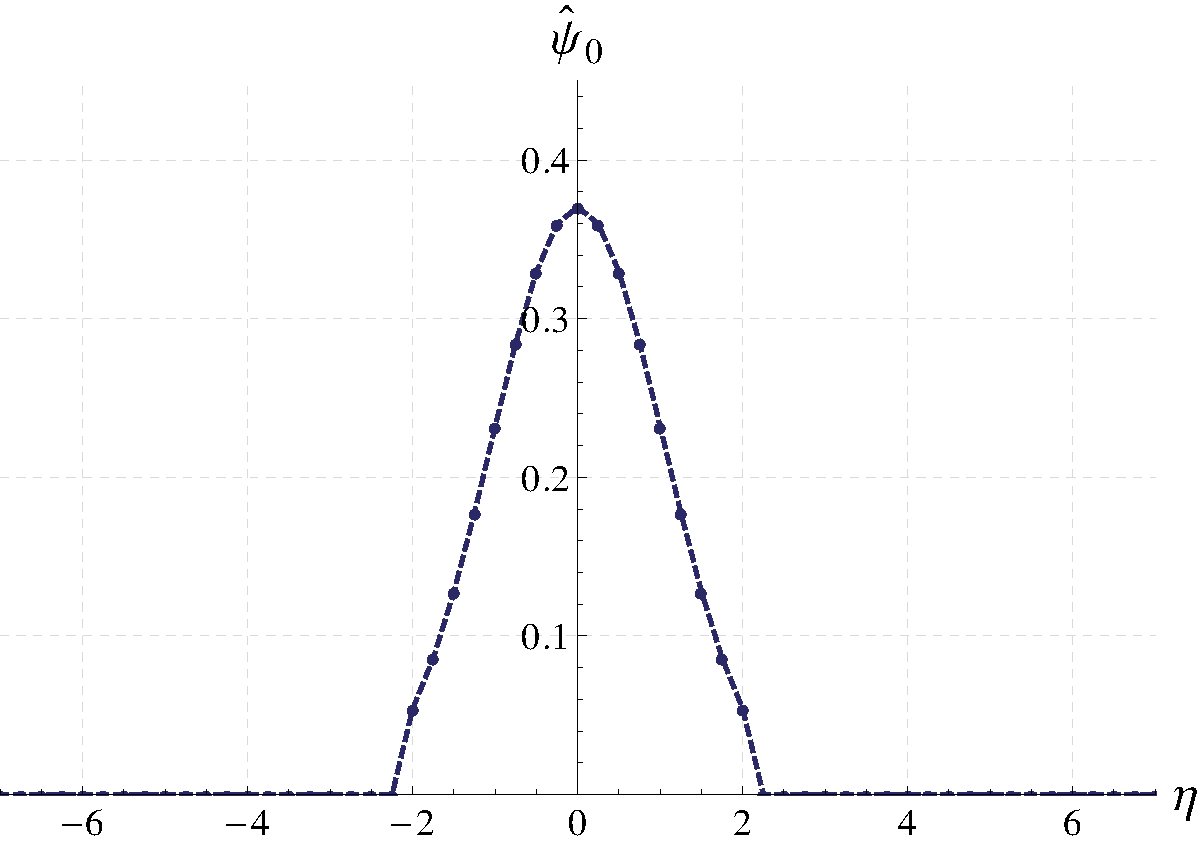
\includegraphics[scale=0.32]{Results/DNA/Eigensystem/T00/0.25/psi_t00_t0_L50_m100_k10_etab2.pdf}} &
\subfloat[$t$=1]{\label{fig:dna_efun_t00_1_delta0.25}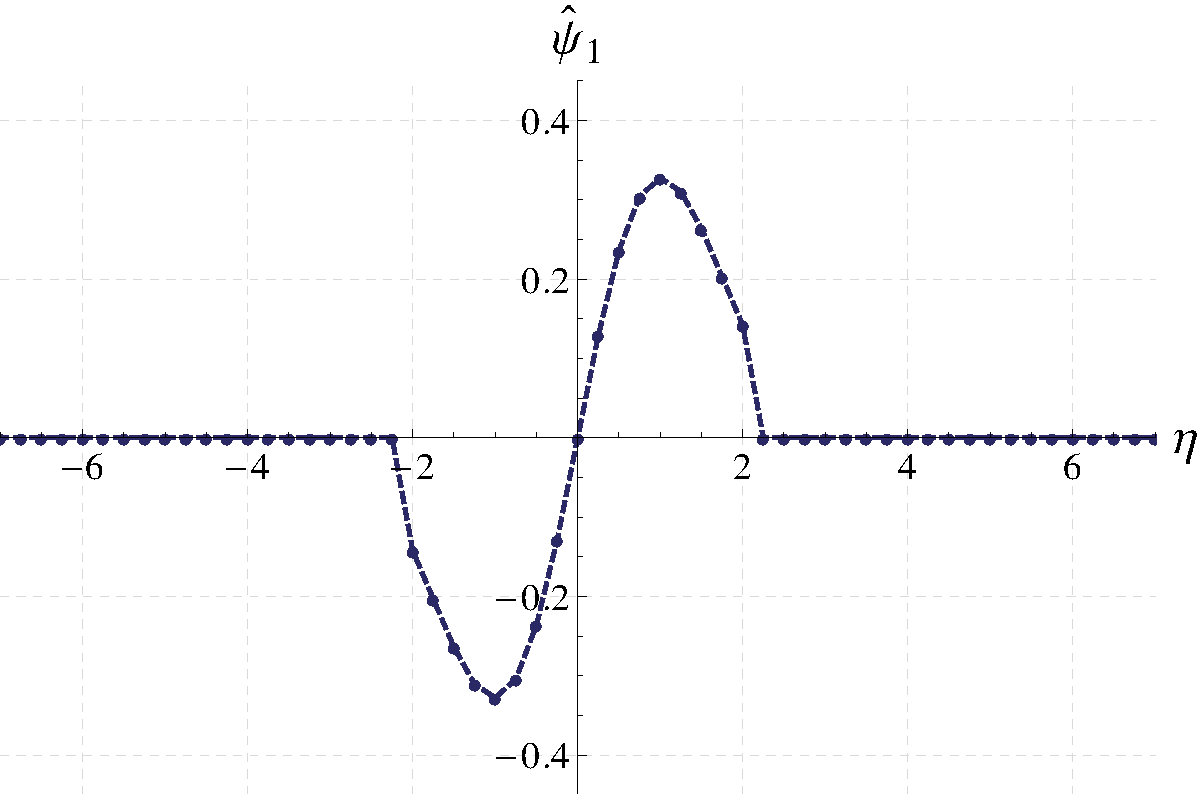
\includegraphics[scale=0.32]{Results/DNA/Eigensystem/T00/0.25/psi_t00_t1_L50_m100_k10_etab2.pdf}} \\
\subfloat[$t$=2]{\label{fig:dna_efun_t00_2_delta0.25}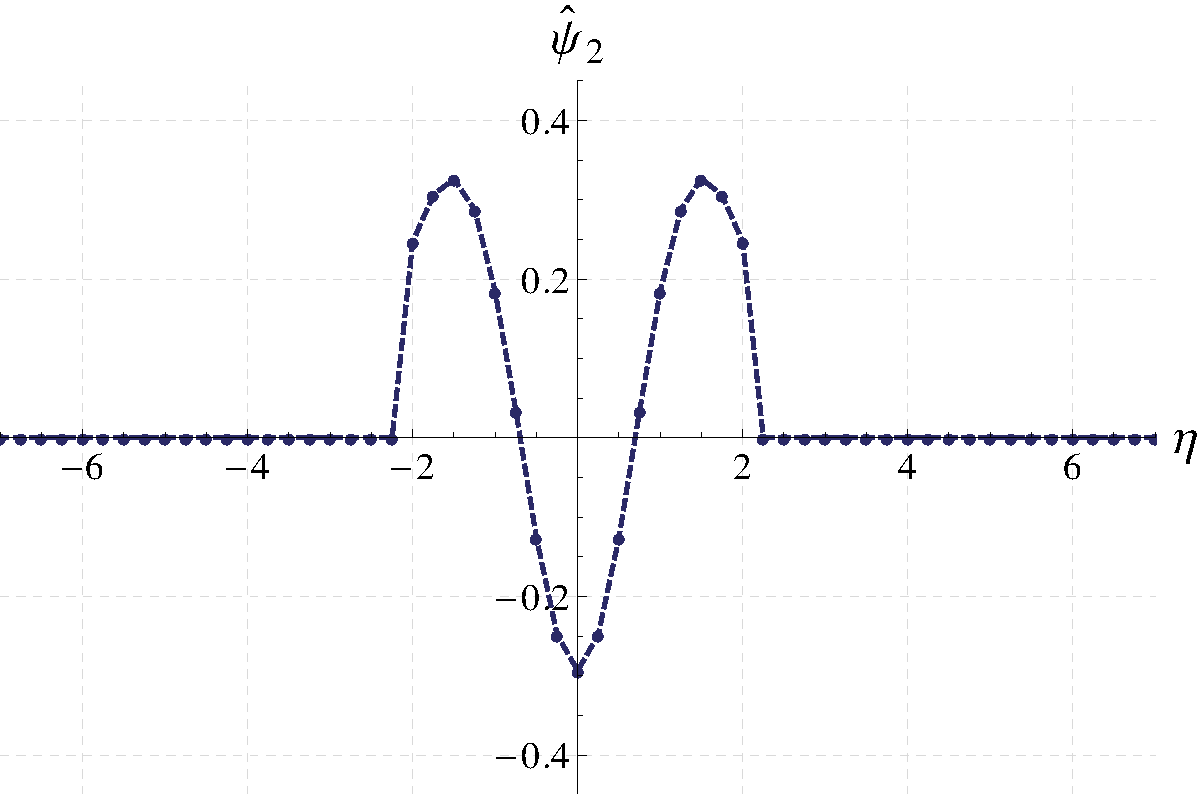
\includegraphics[scale=0.32]{Results/DNA/Eigensystem/T00/0.25/psi_t00_t2_L50_m100_k10_etab2.pdf}} &
\subfloat[$t$=3]{\label{fig:dna_efun_t00_3_delta0.25}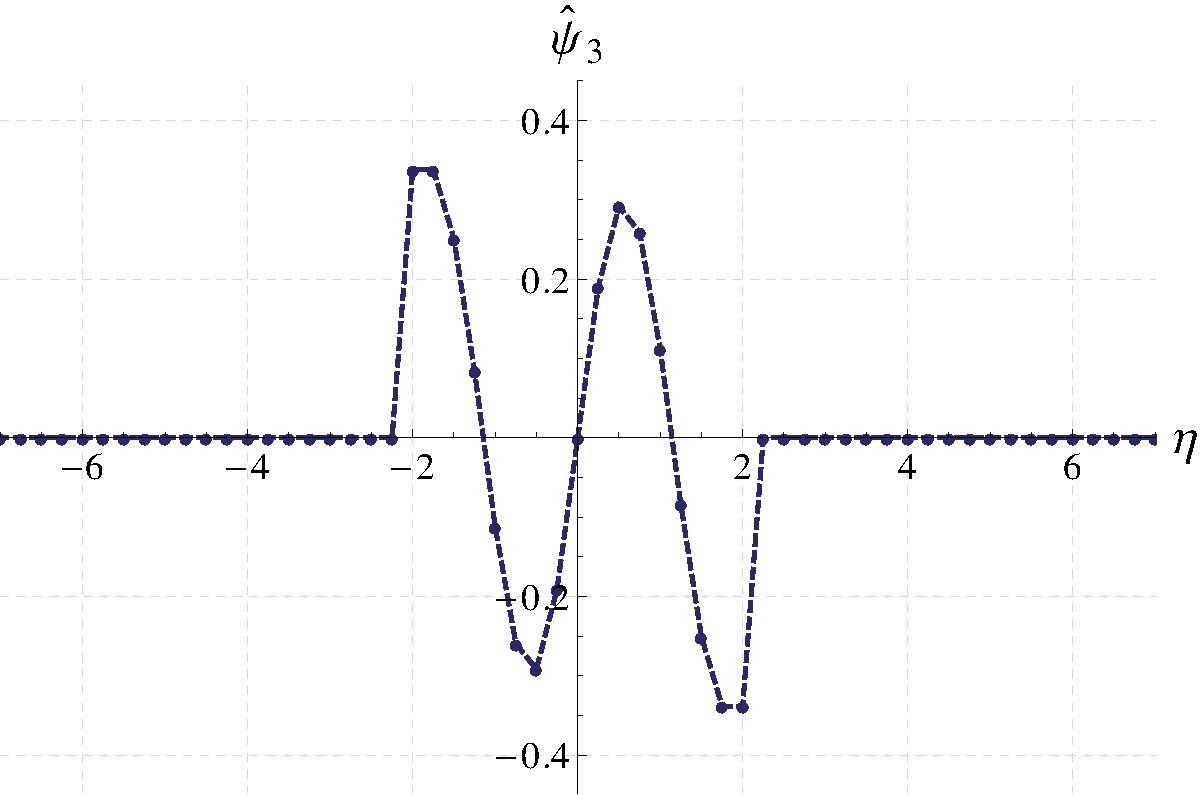
\includegraphics[scale=0.32]{Results/DNA/Eigensystem/T00/0.25/psi_t00_t3_L50_m100_k10_etab2.pdf}}
\end{tabular}
\caption{Eigenfunction plots of $\hat{\psi}_{t}$ with $\Delta=0.25$ ($L$=50 and $m$=100) and $\eta_{B}=2$.}
\label{fig:dna_psi_t00_delta0.25} 
\begin{tabular}{cc}
\subfloat[$t$=0]{\label{fig:dna_efun_t11_0_delta0.25}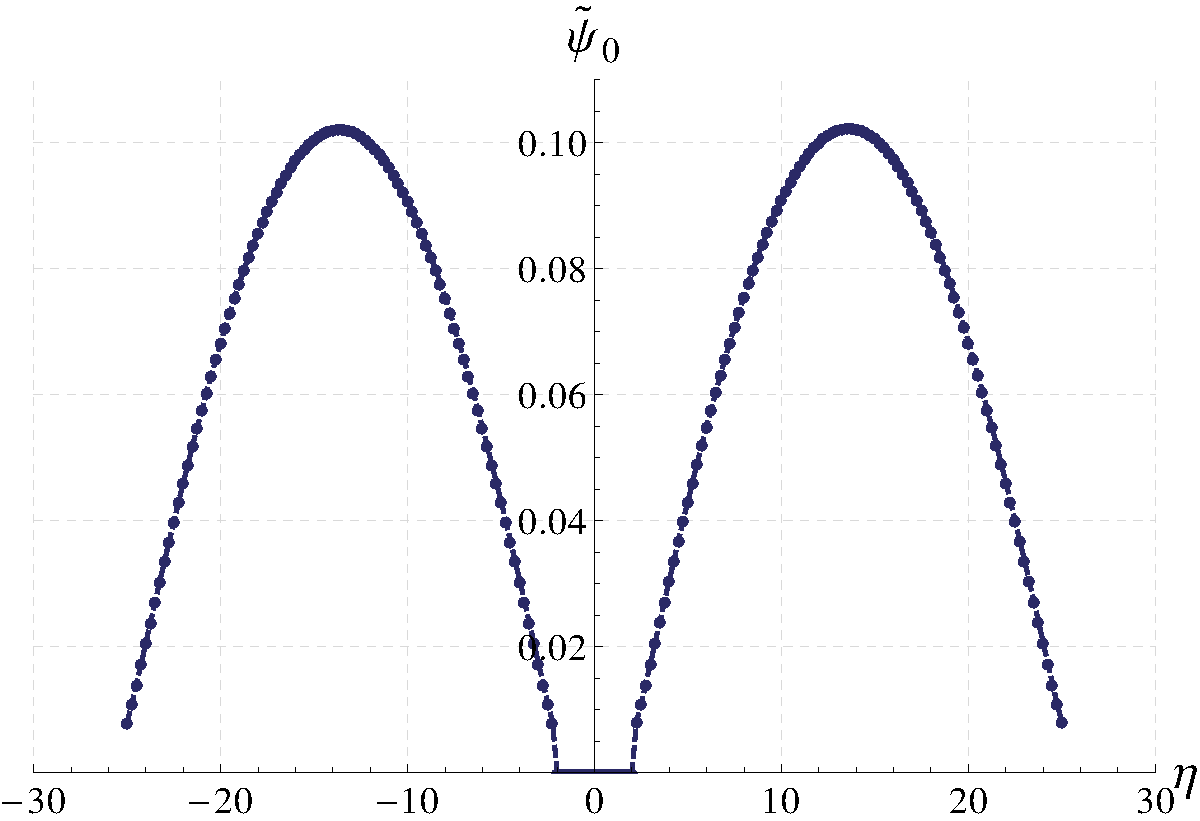
\includegraphics[scale=0.32]{Results/DNA/Eigensystem/T11/0.25/psi_t11_t0_L50_m100_k10_etab2.pdf}} &
\subfloat[$t$=1]{\label{fig:dna_efun_t11_1_delta0.25}\includegraphics[scale=0.32]{Results/DNA/Eigensystem/T11/0.25/psi_t11_t1_L50_m100_k10_etab2.pdf}} \\
\subfloat[$t$=2]{\label{fig:dna_efun_t11_2_delta0.25}\includegraphics[scale=0.32]{Results/DNA/Eigensystem/T11/0.25/psi_t11_t2_L50_m100_k10_etab2.pdf}} &
\subfloat[$t$=3]{\label{fig:dna_efun_t11_3_delta0.25}\includegraphics[scale=0.32]{Results/DNA/Eigensystem/T11/0.25/psi_t11_t3_L50_m100_k10_etab2.pdf}}
\end{tabular}
\caption{Eigenfunction plots of $\tilde{\psi}_{t}$ with $\Delta=0.25$ ($L$=50 and $m$=100) and $\eta_{B}=2$.}
\label{fig:dna_psi_t11_delta0.25} 
\end{figure}

\newpage
\section{Results for DNA Model Calculations}

Results calculated for an intact state of DNA using \eqref{dna_intact} are shown in \figref{dna_intact_etab}. Observing a ladder structure that has all its base pairs intact we calculate free energies for a test case of $N=5$ by using a range of $\eta_B$ and $\kappa/\kappa'$ ratios in order to understand their effect on the ladder structure. Even though a DNA molecule with 5 base pairs is not thermodynamically stable we can still use this small structure to determine the general behaviour of the model. With $\kappa$ being the spring constant of the backbone and $\kappa'$ being the stiffness constant of the base pairs, we change the stiffness constant ratio by varying $\kappa'$ and keeping $\kappa$ fixed. The parameter $\eta_B$ still represents the point at which the base pair bond breaks. 
%
\begin{equation}
\label{fig:free_energy}
F\left(u\right)=-\frac{1}{\beta} \ln Z\left(u\right)
\end{equation}
%
The effect of the parameter $\eta_B$ on the intact state calculations can be seen in Figs.~\ref{fig:dna_intact_etab_0p5}-\ref{fig:dna_intact_etab_2} by the change in the curvature of free energy curves. As we increase the $\eta_B$ limit we are effectively increasing the range of $\eta$ at which a restoring force is felt by the base pair. When the extension $u$ is at the $\eta_B$ limit the bonds break and the restoring force exhibited by the potential vanishes. 

%Results from the free energy calculations for the Intact state are shown in \figref{dna_intact_etab}. These plots were calculated for small $N$ using a range of $\eta$ and $\kappa$ in order to understand their effect on the ladder structure. 

From the dimensionless base pair potential \eqref{dimensionless_dna_pair_potential}, the stiffness constant ratio between the backbone and base pair quantifies the free energy or work needed to apply an extension $u$ to the ladder structure. For $\kappa/\kappa'\approx 1$ we the structure is rather rigid requiring a lot of work to extend the structure, whereas for a high stiffness constant ratio $\kappa/\kappa'\approx 100$ the stiffness constant of the base pairs is much softer, requiring less work for the structure to extend. All of the free energy calculations in \figref{dna_intact_etab} show that reducing $\kappa'$ lowers the free energy curve, this demonstrates that less work was required to extend the ladder structure.

The free energy calculations for different frayed states of the ladder structure are shown in \figref{dna_frayed_etab}. Compared with an intact state, we plot the four different frayed states of a ladder structure with $N=5$, and for various $\eta_B$. Frayed ends of the ladder structure cause an increase of the initial free energy at $u=0$; as we increase $\eta_B$ we find that this increase becomes more noticeable before falling to a minimum. This behaviour can be explained by the compression of the backbone bonds adjacent to the broken base pairs in the ladder structure such that at small $u$ energy is stored in these bonds. For larger $\eta_B$ more work is required to compress the backbone bonds resulting in more energy being stored. This is illustrated well in \figref{dna_frayed_etab_0p5} through to \figref{dna_frayed_etab_1p25} where we see the increase from $\eta_B=0.5$ to $\eta_B=1.25$. As the structure is extended the broken-pairs relax stabilising at a minimum free energy. 

Bubble states in \figref{dna_bubble_etab} have a larger increase in free energies at a given $u$ than frayed states of a similar extent. We attribute this effect to the higher energy cost needed to break the bonds within the ladder structure than at the ends, due to the greater associated distortion of the backbones.

The mean axial displacement calculations in \figref{dna_mxd_etab} highlight the symmetry that exists within the ladder structure. Although we are extending the structure from the $y$ backbone, the equal and opposite reaction force acting on the $x$ backbone results in a symmetry in the calculation of $\langle \eta_{j} \rangle$ shown in \figref{dna_mxd_eta_etab_0p5}, \figref{dna_mxd_eta_etab_1} and \figref{dna_mxd_eta_etab_2}. For all extensions we find that the outermost base pairs extend more than the base pairs within the structure. As we increase the $\eta_B$ parameter in \figref{dna_mxd_etab} we allow the base pairs to extend over a larger range in $\eta$ before breaking, and this results in a larger mean axial displacement for each base pair.

The calculation of average $\xi_{j}$ shown in \figref{dna_mxd_xi_etab_0p5}, \figref{dna_mxd_xi_etab_1} and \figref{dna_mxd_xi_etab_2} draws our attention to the behaviour of the backbones in the ladder structure which is independent of the $\eta_B$ parameter. Using both $\langle \xi_{j} \rangle$ and $\langle \eta_{j} \rangle$ we calculate the average backbone positions $x_{j}$ and $y_{j}$ shown in \figref{dna_mxd_xy}. For each extension we correctly observe the constraints applied by the delta functions with $y_{1}=0$ and $x_{N}=u$.

\begin{figure}[H]
\centering
\begin{tabular}{cc}
\subfloat[$\eta_{B}=0.5$]{\label{fig:dna_intact_etab_0p5}\includegraphics[scale=0.5]{Results/DNA/Intact/kappa_variation/Intact_kappa_variation_L20_m40_etab0p5.pdf}} \\
\subfloat[$\eta_{B}=1$]{\label{fig:dna_intact_etab_1}\includegraphics[scale=0.5]{Results/DNA/Intact/kappa_variation/Intact_kappa_variation_L20_m40_etab1.pdf}} \\
\subfloat[$\eta_{B}=2$]{\label{fig:dna_intact_etab_2}\includegraphics[scale=0.5]{Results/DNA/Intact/kappa_variation/Intact_kappa_variation_L20_m40_etab2.pdf}} 
\end{tabular}
\caption{DNA Model simulations for an intact state of the ladder structure where $N=5$. Simulations are run for a range of cases that vary the $\eta_B$ limit, and the ratios of stiffness constants between the base pair and backbone ($L=20$). The peak in the free energy arises from the periodicity of the extension term in the partition function \eqref{dna_intact}}
\label{fig:dna_intact_etab} 
\end{figure}
 
\begin{figure}[H]
\centering
\begin{tabular}{cc}
\subfloat[$\eta_{B}=0.5$]{\label{fig:dna_frayed_etab_0p5}\includegraphics[scale=0.5]{Results/DNA/Frayed/Frayed_N5_L20_m40_kappa1_etab0p5.pdf}} & 
\subfloat[$\eta_{B}=0.75$]{\label{fig:dna_frayed_etab_0p75}\includegraphics[scale=0.5]{Results/DNA/Frayed/Frayed_N5_L20_m40_kappa1_etab0p75.pdf}} \\ 
\subfloat[$\eta_{B}=0.85$]{\label{fig:dna_frayed_etab_0p85}\includegraphics[scale=0.5]{Results/DNA/Frayed/Frayed_N5_L20_m40_kappa1_etab0p85.pdf}} & 
\subfloat[$\eta_{B}=0.9$]{\label{fig:dna_frayed_etab_0p9}\includegraphics[scale=0.5]{Results/DNA/Frayed/Frayed_N5_L20_m40_kappa1_etab0p9.pdf}} \\
\subfloat[$\eta_{B}=1$]{\label{fig:dna_frayed_etab_1}\includegraphics[scale=0.5]{Results/DNA/Frayed/Frayed_N5_L20_m40_kappa1_etab1.pdf}} & 
\subfloat[$\eta_{B}=1.25$]{\label{fig:dna_frayed_etab_1p25}\includegraphics[scale=0.5]{Results/DNA/Frayed/Frayed_N5_L20_m40_kappa1_etab1p25.pdf}} 
\end{tabular}
\caption{DNA free energy calculations for frayed states of the ladder structure where $N=5$. The label for each frayed state indicates the number of broken base pairs from one end of the ladder structure. Simulations are run for a range of cases that vary the $\eta_B$ limit.}
\label{fig:dna_frayed_etab} 
\end{figure}

\begin{figure}[H]
\centering
\begin{tabular}{cc}
\subfloat[$\eta_{B}=0.5$]{\label{fig:dna_bubble_etab_0p5}\includegraphics[scale=0.35]{Results/DNA/Bubble/Bubble_N5_L20_m40_kappa1_etab0p5.pdf}} & 
\subfloat[$\eta_{B}=0.75$]{\label{fig:dna_bubble_etab_0p75}\includegraphics[scale=0.35]{Results/DNA/Bubble/Bubble_N5_L20_m40_kappa1_etab0p75.pdf}} \\ 
\subfloat[$\eta_{B}=0.85$]{\label{fig:dna_bubble_etab_0p85}\includegraphics[scale=0.35]{Results/DNA/Bubble/Bubble_N5_L20_m40_kappa1_etab0p85.pdf}} & 
\subfloat[$\eta_{B}=0.9$]{\label{fig:dna_bubble_etab_0p9}\includegraphics[scale=0.35]{Results/DNA/Bubble/Bubble_N5_L20_m40_kappa1_etab0p9.pdf}} \\
\subfloat[$\eta_{B}=1$]{\label{fig:dna_bubble_etab_1}\includegraphics[scale=0.35]{Results/DNA/Bubble/Bubble_N5_L20_m40_kappa1_etab1.pdf}} &
\subfloat[$\eta_{B}=1.25$]{\label{fig:dna_bubble_etab_1p25}\includegraphics[scale=0.35]{Results/DNA/Bubble/Bubble_N5_L20_m40_kappa1_etab1p25.pdf}} 
\end{tabular}
\caption{DNA free energy calculations for a bubble states of the ladder structure where $N=5$. The label for each bubbled state indicates the number of intact base pairs, followed by the number of broken base pairs ($intact$, $broken$). For all the bubble states the last remaining base pair is always intact. Calculations are performed for a range of cases that vary the $\eta_B$ limit.}
\label{fig:dna_bubble_etab} 
\end{figure}

\begin{figure}[H]
\centering
\begin{tabular}{cc}
\subfloat[$\eta_{B}=0.5$]{\label{fig:dna_mxd_eta_etab_0p5}\includegraphics[scale=0.5]{Results/DNA/MXD/MXD_eta_N5_L20_m40_kappa1_etab0p5.pdf}} &
\subfloat[$\eta_{B}=0.5$]{\label{fig:dna_mxd_xi_etab_0p5}\includegraphics[scale=0.5]{Results/DNA/MXD/MXD_xi_N5_L20_m40_kappa1_etab0p5.pdf}} \\
\subfloat[$\eta_{B}=1$]{\label{fig:dna_mxd_eta_etab_1}\includegraphics[scale=0.5]{Results/DNA/MXD/MXD_eta_N5_L20_m40_kappa1_etab1.pdf}} &
\subfloat[$\eta_{B}=1$]{\label{fig:dna_mxd_xi_etab_1}\includegraphics[scale=0.5]{Results/DNA/MXD/MXD_xi_N5_L20_m40_kappa1_etab1.pdf}} \\
\subfloat[$\eta_{B}=2$]{\label{fig:dna_mxd_eta_etab_2}\includegraphics[scale=0.5]{Results/DNA/MXD/MXD_eta_N5_L20_m40_kappa1_etab2.pdf}} &
\subfloat[$\eta_{B}=2$]{\label{fig:dna_mxd_xi_etab_2}\includegraphics[scale=0.5]{Results/DNA/MXD/MXD_xi_N5_L20_m40_kappa1_etab2.pdf}} 
\end{tabular}
\caption{Mean axial displacement calculations for the average base pair separation when we apply an extension $u$ on the ladder structure. Simulations are run for an intact state with $\kappa/\kappa'=1$ at different $\eta_B$ limits ($\Delta \approx 0.25$).}
\label{fig:dna_mxd_etab} 
\end{figure}

\begin{figure}[H]
\centering
\begin{tabular}{cc}
\subfloat[$u=\Delta$]{\label{fig:dna_mxd_xy_1delta}\includegraphics[scale=0.75]{Results/DNA/MXD/AveragePosition_N5_L20_m40_kappa1_etab2_u1.pdf}} \\
\subfloat[$u=3\Delta$]{\label{fig:dna_mxd_xy_3delta}\includegraphics[scale=0.75]{Results/DNA/MXD/AveragePosition_N5_L20_m40_kappa1_etab2_u3.pdf}} \\
\subfloat[$u=5\Delta$]{\label{fig:dna_mxd_xy_5delta}\includegraphics[scale=0.75]{Results/DNA/MXD/AveragePosition_N5_L20_m40_kappa1_etab2_u5.pdf}}
\end{tabular}
\caption{Mean axial displacement calculations for the average backbone displacements when we apply an extension $u$ on the ladder structure. Calculations are performed for an intact state with $\kappa/\kappa'=1$ at different extensions ($\Delta \approx 0.25$).}
\label{fig:dna_mxd_xy} 
\end{figure}

\subsection{Conclusion}

From studying the $N=5$ ladder structure we can draw some conclusions on how an applied extension affects the free energy for intact, frayed and bubble states. In all instances applying an extension to the ladder structure moves it away from its equilibrium position due to the work done on the thermodynamic system. This increases the internal energy and consequently the free energy. As we reduce $\kappa'$ less work is required to extend the base pairs within the ladder structure lowering the free energy curve. Here the stiffness constant ratio increases since $\kappa$ is always kept constant.

Broken base pairs in the frayed states move the equilibrium position (minimum free energy) of the ladder structure from $u=0$. As calculations of $\langle \eta \rangle$ have shown, mean base pair separations are not uniform within the structure, and therefore to allow the relaxation of the backbone adjacent to broken base pairs a large enough extension is needed. As the number of broken base pairs increases a larger extension is needed to relax the structure.

The crossover behaviour in free energy curves shown in \figref{dna_frayed_etab_0p85}, \figref{dna_frayed_etab_0p9} and \figref{dna_frayed_etab_1} indicates separate phase transitions for a structure that unzips from one end. Initially, in an intact state at equilibrium, applying an extension from one end disturbs the structure causing the free energy to increase. The base pairs begin to separate with the largest displacements being experienced at the end base pairs. As the extension increases, the intact free energy curve will eventually intersect the first frayed free energy curve implying a phase transition to a frayed structure with a single broken base pair. This process will continue to happen for subsequent frayed states where more base pairs are broken. Following a path of lowest free energy we are able to observe how the base pairs break in a ladder structure from an intact state as the extension $u$ increases. 

The shift in higher free energy curves for bubble states arises from the distorted backbone around each end of the region of broken base pairs within the structure. The shift can be related to the number of broken base pairs that exist. No phase transitions exist for the bubble states as $u$ increases.

\newpage
\section{Results for anharmonic DNA calculations}

In our formulation of the partition function we chose a potential that mechanically described DNA as a harmonic ladder structure. Each base pair experiences a restoring force proportional to a given extension and eventually breaks once the base pair separation reaches the $\eta_B$ limit, at which point the restoring force vanishes. Following the recent work of Prakash et al. who uses the same ladder structure to model DNA we find that their potential on the molecular scale gives a more realistic representation of the base pair  potentials. This potential contains a long range attractive interaction and short range harmonic attraction that resembles our simpler base pair potential when the displacement is small. Expanding the Prakash potential $V_{p}\left(y_{i}\right)$ in ascending powers of $y$ one gets \cite{Prakash2011},
%
\begin{equation}
V_{p}\left(y_{i}\right)=-\epsilon + \frac{1}{2}\left(\frac{12\epsilon}{\sigma^2}\right)y_{i}^2
\end{equation}
%
\begin{equation}
\kappa'= \frac{12\epsilon}{\sigma^2}
\end{equation}
%
where $\epsilon$ is the potential depth, $\sigma$ is the diameter of DNA and $\kappa'$ is the stiffness constant of the base pair. In the limit of $\eta_B \rightarrow \infty$ our potential remains harmonic. To model DNA we adopt Prakash's potential in our partition function where $\eta_B$ now indicates where the base pair bond breaks as it is distorted. 

The results from the first set of calculations compares the shearing force of different molecular lengths with experimental data obtained by Hatch et al. \cite{Hatch2008}. We use a method first employed by Prakash et al. \cite{Prakash2011} where for an intact structure the shear force $f_{s}$ is determined when the average separation of the end base pairs, $\eta_{1}$ and $\eta_{N}$, are equal to our fitting parameter $\eta_{B}$, this is also known as the shearing separation of a single base pair. At the applied extension we are able to determine the dimensionless force $f$ from the partition function by taking the derivative of the free energy with respect to $u$. We find that 
%
\begin{equation}
f\left(u\right)=\frac{1}{\beta}\frac{d\ln Z\left(u\right)}{du}
\end{equation}
%
which can be transformed into a dimensional force by multiplying by a scaling factor $\left(\frac{\kappa k_{B}T}{4}\right)^{\frac{1}{2}}$. The model is dependent on two fitting parameters, $\eta_{B}$ and the base pair stiffness constant $\kappa'$, which we are able to adjust to produce a fit with experimental data. Using a backbone stiffness constant of $\kappa=0.10$ eV/$\text{\AA}^{2}$ \cite{Prakash2011} we can estimate an initial value for $\eta_B$ and $\kappa'$ from data already obtained by Hatch et al.; a stiffness constant ratio of $\kappa/\kappa'=90$ gave a base pair stiffness constant of $\kappa'=0.0011$ eV/$\text{\AA}^{2}$. The shearing separation $\eta_B$ was calculated from the shearing force of a single base pair $f_{bp}$ by taking a differential of the base pair potential at small separations. We find that at room temperature ($T=300$),
%
\begin{equation}
\eta_{B}=\frac{f_{bp}}{\kappa'}\left(\frac{\kappa}{4 k_{B} T}\right)^{\frac{1}{2}} \simeq 2.2
\end{equation}
%
where $f_{bp} = 4$ pN \cite{Hatch2008}. The dimensionless quantity $\eta_{B}$ is converted into real dimensions by the scaling factor $\left(\frac{4k_{B}T}{\kappa}\right)^{\frac{1}{2}}$ to give $\eta'_{B}=\eta_{B}\left(\frac{4k_{B}T}{\kappa}\right)^{\frac{1}{2}} \simeq 2.25\textrm{\AA}$ which is within the acceptable range found in \cite{Prakash2011}. In the DNA model these initial fitting parameters did not agree well with experimental data and therefore had to adjusted to produce a better fit. The results in \figref{dna_large_etab1} show the shear forces for different molecular lengths that produced the best fit with experimental data. These calculations had a $\kappa/\kappa'$ ratio of approximately 150 with a shear force base pair separation of $\eta_B=3.75$. A fit of de Gennes's formula \eqref{deGennes_eq} to Hatch's data \cite{Hatch2008} gave a $\kappa/\kappa' \approx 180$ and $f_{bp} \approx 3.24$ pN ($\eta'_B \approx 3$ \AA).
%
\begin{figure}[H]
\centering
\includegraphics[scale=0.65]{Results/DNA/dna_large_etab/shear_force_large_ksr150_etab3p75.pdf}
\caption{The shear force calculated for various molecular lengths plotted with experimental data. The parameters for these free energy calculations used a stiffness constant ratio of $150$ with $\eta_B = 3.75$. A fit of de Gennes's model (dotted curve) is made with the experimental data. The centre red horizontal line represents the critical force for infinitely long polymers and the upper and lower dashed red lines correspond to 110\% and 90\% of the overstretching transition threshold \cite{Hatch2008}.}
\label{fig:dna_large_etab1} 
\end{figure}
%
In the second set of results we use the first phase transition, the transition from an intact state to a frayed 1 state, to determine the shear force of DNA. Here the $g$ factors within the transfer matrices set the pattern of breakage allowing the mechanics to determine the maximum sustainable shear force of the structure. The free energy curves shown for a sample of different molecular lengths in \figref{dna_frayed_a} and \figref{dna_frayed_c} show the intersection of different free energy curves, highlighting the pathways of breakages that occur in our model, corresponding to the path of minimum free energy as described in section 6.9.1. The results shown in \figref{dna_frayed_shear_force} and \figref{dna} show some of the best fits with experimental data for a range of molecular lengths $N=12,16,20,24,28,32,50$ when we consider the point at which DNA shears to be the first phase transition. These results have a better consistency with the stiffness constant ratios found by Hatch \cite{Hatch2008} even though the results for short DNA do not agree so well with experimental data. 
%
\begin{figure}[H]
\centering
\begin{tabular}{cc}
\subfloat[The shear force calculated for various molecular lengths plotted with experimental data. Parameters for these free energy calculations include a stiffness constant ratio of $\approx 65$ with $\eta_B = 3.75$. A plot of de Gennes model (dotted curve) is made, together with the experimental data.]{\label{fig:dna_frayed_shear_force}\centering\includegraphics[scale=0.7]{Results/DNA/dna/frayed/shear_force_ksr65_etab3p75.pdf}} \\
\subfloat[]{\label{fig:dna_frayed_a}\includegraphics[scale=0.45]{Results/DNA/dna/frayed/N12_Frayed_Analysis_FE.pdf}} 
\subfloat[]{\label{fig:dna_frayed_b}\includegraphics[scale=0.45]{Results/DNA/dna/frayed/N12_Frayed_Analysis_dFE.pdf}} \\
\subfloat[]{\label{fig:dna_frayed_c}\includegraphics[scale=0.45]{Results/DNA/dna/frayed/N16_Frayed_Analysis_FE.pdf}} 
\subfloat[]{\label{fig:dna_frayed_d}\includegraphics[scale=0.45]{Results/DNA/dna/frayed/N16_Frayed_Analysis_dFE.pdf}} 
\end{tabular}
\caption{Free energy curves for the intact state and first few frayed states focusing on specific data points corresponding to $N=12$ and $N=16$. A plot of the dimensionless force corresponding to each free energy curve is illustrated on the right.}
\label{fig:dna_frayed_results} 
\end{figure}
%
\begin{figure}[H]
\centering
\begin{tabular}{cc}
\subfloat[$\kappa/\kappa' = 26$, $\eta_{B}=4.75$]{\label{fig:dna_a}\includegraphics[scale=0.5]{Results/DNA/dna/shear_force_ksr26_etab4p75.pdf}} \\
\subfloat[$\kappa/\kappa' = 46$, $\eta_{B}=4.25$]{\label{fig:dna_b}\includegraphics[scale=0.5]{Results/DNA/dna/shear_force_ksr46_etab4p25.pdf}} \\
\subfloat[$\kappa/\kappa' = 70$, $\eta_{B}=3.50$]{\label{fig:dna_c}\includegraphics[scale=0.5]{Results/DNA/dna/shear_force_ksr70_etab3p5.pdf}} 
\end{tabular}
\caption{Shear force plots for some of the parameters that have close agreements with experimental data. The shear force was calculated from the first phase transition.}
\label{fig:dna} 
\end{figure}

\begin{comment}
\begin{figure}[H]
\centering
\label{fig:dna_frayed_shear_force}\centering\includegraphics[scale=1.0]{Results/DNA/dna/frayed/shear_force_multi.pdf}
\caption{Shear force curves calculated using different free energy intersections for various molecular lengths. The blue data points are calculated using the first free energy intersection (between the intact state and first frayed state), and the purple data points are calculated using the $2^{nd}$ intersection point (between the $1^{st}$ and $2^{nd}$ frayed state). The parameters for these free energy calculations used a stiffness constant ratio of $\sim 65$ with $\eta_B = 3.75$. A fit of de Gennes's model (dotted curve) is made with the experimental data.}
\label{fig:dna_frayed_shear_force} 
\end{figure}

In determining the force-extension behaviour of the structure we compare the shear force using different intersection points in \figref{dna_frayed_shear_force}. We observe that although a complete shear of the structure is more evident from the successive frayed states from \figref{dna_frayed_a}, calculating the shear force from the $n^{th}$ intersection point significantly increases the shear force above the asymptotic limit. Using the first intersection point gives better agreement with experimental results. 
\end{comment}
%
